% TODO
%
% - Refer to Efimov
% - Discuss cohomology classes in Dyckerhoff

\documentclass[english,letter paper,12pt,leqno]{article}
\usepackage{array}
\usepackage{stmaryrd}
\usepackage{amsmath, amscd, amssymb, mathrsfs, accents, amsfonts,amsthm}
\usepackage[all]{xy}
\usepackage{dsfont}
\usepackage{relsize}
\usepackage{tikz}
\def\nicedashedcolourscheme{\shadedraw[top color=blue!22, bottom color=blue!22, draw=gray, dashed]}
\def\nicecolourscheme{\shadedraw[top color=blue!22, bottom color=blue!22, draw=white]}
\def\nicepalecolourscheme{\shadedraw[top color=blue!12, bottom color=blue!12, draw=white]}
\def\nicenocolourscheme{\shadedraw[top color=gray!2, bottom color=gray!25, draw=white]}
\def\nicereallynocolourscheme{\shadedraw[top color=white!2, bottom color=white!25, draw=white]}
\definecolor{Myblue}{rgb}{0,0,0.6}
\usepackage[a4paper,colorlinks,citecolor=Myblue,linkcolor=Myblue,urlcolor=Myblue,pdfpagemode=None]{hyperref}

\usetikzlibrary{snakes}

\SelectTips{cm}{}

\setlength{\evensidemargin}{0.1in}
\setlength{\oddsidemargin}{0.1in}
\setlength{\textwidth}{6.3in}
\setlength{\topmargin}{0.0in}
\setlength{\textheight}{8.5in}
\setlength{\headheight}{0in}

\newtheorem{theorem}{Theorem}[section]
\newtheorem{proposition}[theorem]{Proposition}
\newtheorem{lemma}[theorem]{Lemma}
\newtheorem{corollary}[theorem]{Corollary}
\newtheorem{setup}[theorem]{Setup}

% Labels in tabular
\newcommand{\tagarray}{\mbox{}\refstepcounter{equation}$(\theequation)$}

\newtheoremstyle{example}{\topsep}{\topsep}
	{}
	{}
	{\bfseries}
	{.}
	{2pt}
	{\thmname{#1}\thmnumber{ #2}\thmnote{ #3}}
	
	\theoremstyle{example}
	\newtheorem{definition}[theorem]{Definition}
	\newtheorem{example}[theorem]{Example}
	\newtheorem{remark}[theorem]{Remark}
	\newtheorem{strat}[theorem]{Strategy}

\numberwithin{equation}{section}

% Operators
\def\AA{\mathcal{A}}
\def\BB{\mathcal{B}}
\def\HH{\HH}
\def\HH{\mathcal{H}}
\def\ob{\operatorname{ob}}
\def\eval{\operatorname{ev}}
\def\res{\operatorname{Res}}
\def\Coker{\operatorname{Coker}}
\def\Ker{\operatorname{Ker}}
\def\im{\operatorname{Im}}
\def\can{\operatorname{can}}
\def\K{\mathbf{K}}
\def\D{\mathbf{D}}
\def\N{\mathbf{N}}
\def\LG{\mathcal{LG}}
\def\Ab{\operatorname{Ab}}
\def\stab{\operatorname{stab}}
\def\Hom{\operatorname{Hom}}
\def\modd{\operatorname{mod}}
\def\Modd{\operatorname{Mod}}
\def\be{\begin{equation}}
\def\ee{\end{equation}}
\def\nN{\mathds{N}}
\def\nZ{\mathds{Z}}
\def\nQ{\mathds{Q}}
\def\nR{\mathds{R}}
\def\nC{\mathds{C}}
\def\jac{\operatorname{Jac}_W}
\DeclareMathOperator{\Ext}{Ext}
\DeclareMathOperator{\Tr}{Tr}
\DeclareMathOperator{\End}{End}
\DeclareMathOperator{\rank}{rank}
\DeclareMathOperator{\tot}{Tot}
\DeclareMathOperator{\ch}{ch}
\DeclareMathOperator{\str}{str}
\DeclareMathOperator{\hmf}{hmf}
\DeclareMathOperator{\HMF}{HMF}
\DeclareMathOperator{\mfdg}{mf}
\DeclareMathOperator{\Spec}{Spec}
\DeclareMathOperator{\At}{At}
\DeclareMathOperator{\HF}{HF}
\DeclareMathOperator{\sigmastar}{\sigma_t}
\DeclareMathOperator{\vAt}{At}

\begin{document}

% Commands
\def\Res{\res\!}
\newcommand{\ud}{\mathrm{d}}
\newcommand{\Ress}[1]{\res_{#1}\!}
\newcommand{\cat}[1]{\mathcal{#1}}
\newcommand{\lto}{\longrightarrow}
\newcommand{\xlto}[1]{\stackrel{#1}\lto}
\newcommand{\md}[1]{\mathscr{#1}}
\newcommand{\coeff}[1]{\widetilde{#1}}
\def\sus{\l}
\def\l{\,|\,}
\def\sgn{\textup{sgn}}
\def\samp{\zeta}
\def\Samp{Z}
\def\traff{N}

\title{Constructing $A_\infty$-categories of matrix factorisations}
\author{Daniel Murfet}

\maketitle

\begin{abstract}
We study constructive $A_\infty$-models of the DG-category of matrix factorisations of a potential over a commutative $\mathbb{Q}$-algebra $k$, consisting of a Hom-finite $A_\infty$-category equipped with an $A_\infty$-idempotent functor.
\end{abstract}

\tableofcontents

\section{Introduction}

This paper continues the project begun in \cite{pushforward,cut,lgdual} of making the theory of affine B-twisted topological Landau-Ginzburg models \emph{constructive}, in the sense of deriving formulas and algorithms which compute the fundamental categorical structures from coefficients of the potential and the differentials of matrix factorisations. For example, the units and counits of adjunction in the bicategory of Landau-Ginzburg models \cite{lgdual} and the pushforward and convolution operations \cite{pushforward} may be described in terms of various flavours of Atiyah classes.

In this paper we study \emph{idempotent finite $A_\infty$-models} of DG-categories of matrix factorisations over arbitrary $\mathbb{Q}$-algebras $k$. An idempotent finite model of a DG-category $\AA$ over $k$ is a pair $(\mathcal{B}, E)$ consisting of an $A_\infty$-category $\mathcal{B}$ over $k$ which is Hom-finite, in the sense for each pair $X,Y$ of objects the complex $\mathcal{B}(X,Y)$ is a finitely generated projective $k$-module, together with a diagram of $A_\infty$-functors
\[
\xymatrix@C+3pc{
\AA \ar@<1ex>[r]^I & \mathcal{B} \ar@(ur,dr)^E \ar@<1ex>[l]^P
}
\]
with $A_\infty$-homotopies $P \circ I \simeq 1$ and $I \circ P \simeq E$. Using the finite pushforward construction of \cite{pushforward} and Clifford actions of \cite{cut} we explain how to define an idempotent finite $A_\infty$-model of the DG-category of matrix factorisations $\AA$ of any potential $W$ over $k$. When $k$ is a field this is constructive in the sense that we give algorithms for computing the entries in the higher multiplications on $\BB$ and the components of $E$, viewed as matrices, from the Atiyah class of $\AA$ and a Gr\"obner basis of the defining ideal of the critical locus of $W$.

We note that our goal is \emph{not} to construct a minimal model: $\BB$ has nonzero differential. When $k$ is a field the usual approach to finding a Hom-finite $A_\infty$-model of $\AA$ is to equip $H^*(\AA)$ with an $A_\infty$-structure, so that there is a diagram of $A_\infty$-functors
\[
\xymatrix@C+3pc{
\AA \ar@<1ex>[r]^I & H^*(\AA) \ar@<1ex>[l]^P
}
\]
and $A_\infty$-homotopies $P \circ I \simeq 1$ and $I \circ P \simeq 1$. The problem with this approach is that the minimal model is only under good control for those matrix factorisations $X,Y$ where we happen to know a good cohomological splitting on $\AA(X,Y)$. An important example is the case where $X = Y = k^{\stab}$ is the standard generator, where the resulting $A_\infty$-structure has been studied by Seidel \cite{??}, Dyckerhoff \cite{??}, Efimov \cite{??}, Sheridan \cite{??}, Shklyarov \cite{??} and recently Tu \cite{??}. However the generator is a rather special object: for general objects, and when the base ring $k$ is not a field, if we want to find a constructive Hom-finite $A_\infty$-model of $\AA$ it seems that relying on natural cohomological splittings is the wrong approach. One alternative is the idempotent finite model presented below, and a related idea has been developed in the complex analytic setting by Shklyarov \cite{??}.
\\

Let us consider the DG-category $\AA = \mfdg(R,W)$ of finite-rank matrix factorizations of a potential $W \in R = k[x_1,\ldots,x_n]$ over an arbitrary $\mathbb{Q}$-algebra $k$. This is a DG-category over $R$, which we can view as a $\nZ_2$-graded $R$-module
\[
\HH_{\AA} = \bigoplus_{X,Y} \AA(X,Y)
\]
equipped with some $R$-linear structure, namely, the differential $\mu_1$ and composition operator $\mu_2$. Let $\varphi: k \lto R$ denote the inclusion of constants. We can ask if the restriction of scalars $\varphi_*( \HH_{\AA} )$ is $A_\infty$-homotopy equivalent over $k$ to an $A_\infty$-category which is Hom-finite over $k$, and can such a finite model be described constructively? This is related to the problem of pushforwards considered in \cite{pushforward} and as there it is unclear that in general a \emph{direct} construction of the finite pushforward exists.

Instead, following \cite{pushforward} the conceptual approach we adopt here is to seek an algorithm which constructs both a larger object $\mathcal{B}$ which is a Hom-finite $A_\infty$-category over $k$ together with an idempotent $E: \mathcal{B} \lto \mathcal{B}$ which splits to $\AA$. More precisely, the larger object is obtained by adjoining to $\AA$ a number of odd supercommuting variables $\theta_1,\ldots,\theta_n$ and completing along the the critical locus of $W$ to obtain the DG-category
% The usual prescription for computing minimal models when $k$ is a field is to somehow choose an collection of splittings of short exact sequences to define a homotopy equivalence between $H^*(\AA)$ and $\AA$. From our point of view the main drawback of this approach is that the minimal model thus obtained is not constructive: the higher operations on $H^*(\AA)$ depend on choosing representative cocycles for a basis of the cohomology and these choices cannot be made constructively from the input data (by which we mean the coefficients of the potential and the differentials of the matrix factorisations involved).\footnote{Well when $k$ is a field you can use Gr\"obner basis methods to compute a basis, of course, so you could argue there \emph{is} an algorithm, and moreover many of the existing methods just take a matrix factorisation as input then compute cohomology and so on. So we need to be more precise here. It's something like: in the Gr\"obner basis algorithm you essentially invert certain coefficients, so you only get rational functions on the set of potentials and matrix factorisations whereas our construction is polynomial.}
\[
\AA_\theta = \bigwedge F_\theta \otimes_k \AA \otimes_R \widehat{R}\,,
\]
where $F_\theta$ is the $\nZ_2$-graded $k$-module $\bigoplus_{i=1}^n k \theta_i$ which is concentrated in odd degree, and $\widehat{R}$ denotes the $I$-adic completion where $I = (\partial_{x_1} W, \ldots, \partial_{x_n} W)$. The differential on $\AA_\theta$ is the one inherited from $\AA$. Note that the completion $\AA \otimes_R \widehat{R}$ can be recovered from $\AA_\theta$ by splitting the idempotent DG-functor on $\AA_\theta$ which arises from the morphism of algebras
\be\label{eq:projector_e}
\bigwedge F_\theta \lto k \cdot 1 \lto \bigwedge F_\theta
\ee
which projects onto the identity by sending all $\theta$-forms of nonzero degree to zero.

One is supposed to think of $F_\theta$ as the normal bundle to the critical locus of $W$, and $\AA_\theta$ can be equipped with a natural strong deformation retract which arises from a connection $\nabla$ differentiating in the normal directions to the critical locus. Applying the homological perturbation lemma to this data results in a Hom-finite $A_\infty$-category $\BB$ with
\[
\BB(X,Y) = R/I \otimes_R \Hom_R(X,Y)\,.
\]
By construction there is an idempotent finite $A_\infty$-model
\[
\xymatrix@C+3pc{
\AA \otimes_R \widehat{R}\, \ar@<1ex>[r]^-I & \mathcal{B} \ar@(ur,dr)^E \ar@<1ex>[l]^-P
}
\]
of the completion $\AA \otimes_R \widehat{R}$, which we show is homotopy equivalent to $\AA$ over $k$ (in particular $\AA$ and $\AA \otimes_R \widehat{R}$ are both DG-enhancements of the $k$-linear triangulated category $\hmf(R,W)$, and arguably the completion is the more natural of the two). Here the $A_\infty$-idempotent $E$ arises in the obvious way as the transfer to $\BB$ of the idempotent \eqref{eq:projector_e}. Finally, there is an algorithm which presents the higher multiplications of $\BB$ and the components of $E$ in terms of Feynman diagrams, in which the local interactions arise from the components of the operator $[d_{\AA}, \nabla]$ on $\AA_{\theta}$ (the Atiyah class of $\AA$), and iterated Euclidean division with respect to a Gr\"obner basis of $I$.

As a final remark, we note that if a matrix factorisation $X$ can be built in the triangulated category of matrix factorisations from $k^{\stab}$, then knowing the $A_\infty$-minimal model of $\AA(k^{\stab},k^{\stab})$ could allow us in principle to calculate the $A_\infty$-minimal model of $\AA(X,X)$. In practice, however, the differential $d_X$ is a small matrix but the algorithm for constructing $X$ from $k^{\stab}$ is complicated, so it is not clear that this is of much use.

%A minimal model for $\AA$ exists over $k$ (which we recall, is not a field) if and only if this idempotent splits, and so any algorithm for splitting this idempotent is an algorithm for producing the minimal model. The tuple $(R/I \otimes_R \AA, \{m_n\}_{n \ge 1}, \widetilde{e})$ consists of the data of an infinite sequence of tensors defining the $m_n$ and the components of $\widetilde{e}$, and given a choice of $k$-basis of $R/I$ and $R$-basis of the matrix factorisations involved, the coefficients of these tensors are given constructively in terms of the input data (for example, we will informally describe a Turing machine which computes them). This tuple is what we mean by a \emph{constructive} finite presentation of $\AA$.\footnote{Calculating beyond this point involves Gaussian eliminations and thus regular functions of the input data - the output and nature of the cohomology classes varies across strata defined by the vanishing of the denominators in such functions.}

%\textbf{Relations to earlier work.} While the category of perfect modules over the minimal model of the generator is equivalent to the homotopy category of matrix factorisations, this does not appear to be a practical approach to finding the minimal model of the endomorphism DG-algebra of a generic matrix factorisation $X$, because one needs to know a compact presentation of $X$ as a twisted complex over the generator, and determining such presentations is a hard problem in itself. %One reason to go beyond generators is that it is appears to be difficult, in general, to explicitly present a given matrix factorization as a twisted complex over the generator.

%The problem of constructing $\mathscr{U}_Z$ can be approached on an ad hoc basis, but at least for those TFTs whose algebraic data arises from homological algebra, there is a principled approach similar to the one espoused for constructive algebraic topology in \cite{constructat}. The idea is to arrange for every homological object which appears in the calculation of $Z(M)$ from $M$ to be paired with a finite model via a strong deformation retract; such pairings are referred to as \emph{objects with effective homology} in \cite{constructat, constructat2}. %Since all steps in calculating $Z(M)$ will naturally construct new finite models and new strong deformation retracts, the execution of $\mathscr{U}_Z$ may be modelled as a series of reductions in the sense of \cite{constructat}.

%In typical cases of geometric origin, for instance topological Landau-Ginzburg models, the morphisms $M$ in the bordism category may be smoothly varied - for instance, if the defect conditions arise in continuous families. It is natural, therefore, to ask about the derivatives of the functor $Z$ with respect to these parameters. One way to make sense of this problem is via $A_\infty$-categories and differential linear logic \cite{??,??}, and for the particular case of Landau-Ginzburg models, this paper provides the relevant effective models.

\vspace{0.3cm}

\emph{Acknowledgements.} Thanks to Calin Lazaroiu for encouragement, inspiration and many conversations about $A_\infty$-structures.

\vspace{0.3cm}

\textbf{TODO:}

\begin{itemize}

%\item More Lazaroiu references, eg for topological string and the role of $A_\infty$-categories there.

%\item Can we really say we have an algorithm outside the Koszul case?

%\item Emphasise that our propagators are Atiyah classes (a kind of curvature). %For Feynman diagrams and Atiyah class as propagator see p.42 of the generating the super potential paper. Our paper should have lots of references to the recent Lazaroiu output
\item At vs $\vAt_{\AA}$

\item Cite Lazaroiu for constructive

\item Replace hand-drawn diagrams

\item Define trees, branch denotation, evaluation.

\item Treat $\Gamma$ in diagrams (or at least talk about it)

\item Emphasise intuition about virtual particles being excitations in the direction away from the code subspace.

\item Relate to Tu, Shklyarov.

%\item Give the semi-universal deformation of the cusp as an example of a potential

%\item Our models are ``Clifford enriched'' in a weak sense.
% Constructive means: we have a finite-dimensional thing, we choose a basis, and there is an algorithm for computing the entries in that matrix. What we currently have in mind is “varies well with deformations” and “doesn’t rely on computing cohomology and having that be free”

% \item Well actually our finite model is all given in terms of explicit polynomials (although admittedly they are huge opaque sums) but still you can’t say that about the other approaches

% Maybe the real point is that once you choose a basis for the cohomology, it is not clear that the propagator in your Feynman diagrams (which is the most important thing in QFT, i.e. that is where you really see what kind of particle you are dealing with) has any clear relation to the matrix factorisations involved. Of course either way (our way or the highway) doing \emph{actual} calculations is difficult, but in QFT you prove general theorems by reasoning about the kinds of particles involved, and that boils down to a clear understanding of the propagators. In our approach, the propagator is the Atiyah class, which by our earlier work can be understood as the central homological avatar of a matrix factorisation. So it is conceptually clean. Especially in the case of the generator where you can eliminate the exponentials.

% Answer the question: what about minimal models? Does it apply to power series rings?
\end{itemize}

% Note that as in Weinberg we group certain sums of creation and annihilation operators together as $\psi(x)$ rather than splitting it into summands and calling each one an interaction vertex. There are many presentations.

%\begin{remark} Here is a novel model of cut
%\[
%W \lto V \lto U
%\]
%begin with $X$, a $\cat{A}_V$-$\cat{A}_W$-bimodule, $Y$ a $\cat{A}_U$-$\cat{A}_V$-bimodule. Turn these into MFs
%\begin{align*}
%|X| = k^{\stab}_{V - W} \otimes X\\
%|Y| = k^{\stab}_{U - V} \otimes Y
%\end{align*}
%That is, execute the algorithms. Then tensor $|Y| \otimes |X|$. Then go back again, to compute the minimal model.
%\end{remark}

\section{Background}

Throughout $k$ is a commutative $\mathbb{Q}$-algebra and unless specified otherwise $\otimes$ means $\otimes_k$. If $\bold{x} = (x_1,\ldots,x_n)$ is a sequence of formal variables then $k[\bold{x}]$ denotes $k[x_1,\ldots,x_n]$ and similarly for power series rings. Given $M \in \mathbb{N}^n$ we write $x^M$ for $x_1^{M_1} \cdots x_n^{M_n}$. 

Let $R$ be a commutative ring. Given finite-rank free $\nZ_2$-graded $R$-modules $M, N$ and $\phi \in \Hom_R(M,N)$ we say that $\phi$ is \emph{even} (resp. \emph{odd}) if $\phi(M_i) \subseteq N_i$ (resp. $\phi(M_i) \subseteq N_{i+1}$) for all $i \in \nZ_2$. This makes $\Hom_R(M,N)$ into a $\nZ_2$-graded $R$-module. Given two homogeneous operators $\psi, \phi$ the \emph{graded commutator} is
\be
[\phi, \psi] = \phi \psi - (-1)^{|\phi||\psi|} \psi \phi\,.
\ee
In this note all operators are given a $\nZ_2$-grading and the commutator always denotes the graded commutator. We briefly recall some important operators on exterior algebras
\[
\bigwedge F_\xi = \bigwedge \bigoplus_{i=1}^r k \xi_i
\]
where $F_\xi = \bigoplus_{i=1}^r k \xi_i$ denotes a free $k$-module of rank $r$ with basis $\xi_1,\ldots,\xi_r$. We give $F_\xi$ a $\nZ_2$-grading by assigning $|\xi_i| = 1$, that is, $F_\xi \cong k^{\oplus r}[1]$. The inherited $\nZ_2$-grading on $\bigwedge F_\xi$ is the reduction mod $2$ of the usual $\nZ$-grading on the exterior algebra, e.g. $|\xi_1 \xi_2| = 0$.

We define odd operators $\xi_j \wedge (-), \xi_j^* \,\lrcorner\, (-)$ on $\bigwedge F_\xi$ by wedge product and contraction, respectively, where contraction is defined by the formula
\begin{align*}
\xi_j^* \,\lrcorner\, \Big( \xi_{i_1} \cdots \xi_{i_s} \Big) = \sum_{l=1}^s (-1)^{l-1} \delta_{j, i_l} \xi_{i_1} \wedge \cdots \wedge \widehat{ \xi_{i_l} } \wedge \cdots \wedge \xi_{i_s}\,.
\end{align*}
Often we will simply write $\xi_j$ for $\xi_j \wedge (-)$ and $\xi_j^*$ for $\xi_j^* \,\lrcorner\, (-)$. Clearly with this notation, as operators on $\bigwedge F_\xi$, we have the commutator (as always, graded)
\be\label{eq:wedge_contract_comm}
\big[ \xi_i, \xi_j^* \big] = \xi_i \xi_j^* + \xi_j^* \xi_i = \delta_{ij} \cdot 1\,.
\ee
and also $[ \xi_i, \xi_j ] = [\xi_i^*, \xi_j^*] = 0$.

\subsection{$A_\infty$-categories}\label{section:ainfcat}

For the theory of $A_\infty$-categories we follow the notational conventions of \cite[\S 2]{lazaroiu}, which we now recall. Another good reference is Seidel's book \cite{seidel}. A small $\nZ$-graded $A_\infty$-category $\cat{A}$ over $k$ is specified by a set of objects $\operatorname{ob}(\cat{A})$ and $\nZ$-graded $k$-modules $\AA(a,b)$ for any pair $a,b \in \operatorname{ob}(\cat{A})$ together with $k$-linear maps
\[
\mu_{a_n,\ldots,a_0}: \AA(a_{n-1}, a_n) \otimes \cdots \otimes \AA(a_0, a_1) \lto \AA(a_0,a_n)
\]
of degree $2 - n \equiv n$ for every sequence of objects $a_0,\ldots,a_n$ with $n \ge 0$. If the objects involved are clear from the context, we will write $\mu_n$ for this map. These maps are required to satisfy the following equation for $n \ge 1$
\be\label{eq_ainf_constraints}
\sum_{\substack{i \ge 0, j \ge 1 \\ 1 \le i + j \le n}} (-1)^{ij + i + j + n} \mu_{n-j+1}\Big( x_n \otimes \cdots \otimes x_{i+j+1} \otimes \mu_j( x_{i+j} \otimes \cdots \otimes x_{i+1} ) \otimes x_i \otimes \cdots \otimes x_1 \Big) = 0
\ee
In particular we have a degree zero map
\[
\mu_2 = \mu_{cba}: \AA(b,c) \otimes \AA(a,b) \lto \AA(a,c)
\]
which satisfies the $n = 3$ equation
\begin{align*}
- &\mu_2( x \otimes \mu_2( y \otimes z ) ) + \mu_2( \mu_2( x \otimes y ) \otimes z ) + \mu_1 \mu_3( x \otimes y \otimes z )\\
& + \mu_3( \mu_1(x) \otimes y \otimes z ) + \mu_3( x \otimes \mu_1(y) \otimes z ) + \mu_3( x \otimes y \otimes \mu_1(z) ) = 0
\end{align*}
expressing that $\mu_2$ is associative up to the homotopy $\mu_3$ relative to the differential $\mu_1$. The operators $\mu_n$ are sometimes referred to as \emph{higher multiplications}. Any DG-category is an $A_\infty$-category where $\mu_1$ is the differential, $\mu_2$ is the composition and $\mu_n = 0$ for $n \ge 3$. Note that a DG-category has identity maps $u_a \in \AA^0(a,a)$ for all objects $a$, and these make $\cat{A}$ a \emph{strictly unital} $A_\infty$-category \cite[\S 2.1]{lazaroiu}, \cite[\S I.2]{seidel}.

To minimise the pain of working with $A_\infty$-categories, it is convenient to adopt a different point of view on the higher operations, which eliminates most of the signs: from the $\mu$ we can define \emph{suspended forward compositions} \cite[\S 2.1]{lazaroiu}
\be
r_{a_0,\ldots,a_n}: \AA(a_0, a_1)[1] \otimes \cdots \otimes \AA(a_{n-1}, a_n)[1] \lto \AA(a_0,a_n)[1]
\ee
for which the $A_\infty$-constraints \eqref{eq_ainf_constraints} take the more attractive form
\[
\sum_{\substack{i \ge 0, j \ge 1 \\ 1 \le i + j \le n}} r_{a_0, \ldots, a_i, a_{i+j}, \ldots, a_n} \circ \Big( \operatorname{id}_{a_0a_1} \otimes \cdots \otimes \operatorname{id}_{a_{i-1}a_i} \otimes r_{a_i,\ldots,a_{i+j}} \otimes \operatorname{id}_{a_{i+j}a_{i+j+1}} \otimes \cdots \otimes \operatorname{id}_{a_{n-1}a_n} \Big) = 0
\]
As before we write $r_n$ for $r_{a_0,\ldots,a_n}$ if the indices are clear. Note that while $\mu_n$ has $\nZ_2$-degree $n$, the $r_n$'s are all odd operators. The $\nZ_2$-degree of a homogeneous element $x \in \AA(a,b)$ will be denoted $|x|$ and we write $\widetilde{x} = |x| + 1$ for the degree of $x$ viewed as an element of $\AA(a,b)[1]$. Sometimes we refer to this as the \emph{tilde grading}. We refer the reader to \cite{lazaroiu} for the definition of the suspended forward compositions, but note $\mu_1(x) = r_1(x)$ and
\be\label{eq:mu2vsr2}
\mu_2(x_1 \otimes x_2) = (-1)^{\widetilde{x}_1\widetilde{x}_2 + \widetilde{x}_1 + 1} r_2(x_2 \otimes x_1)\,.
\ee
The Koszul sign rule always applies when we evaluate the application of a tensor product of homogeneous linear maps on a tensor, for example since $r_2$ is odd, the map
\[
1 \otimes r_2: \AA(a,b)[1] \otimes \AA(b,c)[1] \otimes \AA(c,d)[1] \lto \AA(a,b)[1] \otimes \AA(b,d)[1]
\]
applied to a tensor $x_3 \otimes x_2 \otimes x_1$ is
\[
(1 \otimes r_2)(x_3 \otimes x_2 \otimes x_1) = (-1)^{\widetilde{x_3}} x_3 \otimes r_2( x_2 \otimes x_1 )
\]
where we had to know that the domain involved $\AA(a,b)[1]$ rather than $\AA(a,b)$ to know that we were supposed to use the tilde grading on $x_3$. %This information will be clear from the context.

We also use the sector decomposition of \cite[\S 2.2]{lazaroiu}. We associate to $\cat{A}$ the $k$-module
\[
\HH_{\cat{A}} = \bigoplus_{a,b \in \operatorname{ob}(\cat{A})} \AA(a,b)
\]
equipped with the induced $\nZ_2$-grading. Let $Q$ be the commutative associative $k$-algebra (without identity) generated by $\epsilon_a$ for $a \in \operatorname{ob}(\cat{A})$ subject to the relations $\epsilon_a \epsilon_b = \delta_{ab} \epsilon_a$ (this non-unital algebra is denoted $R$ in \cite{lazaroiu}). Then $\HH_{\cat{A}}$ has a $Q$-bimodule structure which encodes the decomposition of $\HH_{\cat{A}}$ according to pairs $a,b$ (TODO)

We denote by $\widetilde{\otimes}$ the tensor product obtained using the opposite $Q$-bimodule structure so
\begin{align*}
\HH^{\otimes_Q k} &= \bigoplus_{X_0,\ldots,X_k} \HH(X_k,X_{k-1}) \otimes \cdots \otimes \HH(X_1,X_0)
\end{align*}

\subsection{Homological perturbation}

We will not give a full exposition of the homological perturbation lemma here, but we do need to fix some notation. What we call a \emph{deformation retract} in \cite{cut} is called a \emph{strict deformation retract} in \cite[\S 3.3]{lazaroiu}, with $P = \pi \sigma$.

Explain the connection to minimal models etc. Just reference Lazaroiu for the homological perturbation construction (also Seidel) but explain the branch denotation.

\section{The idempotent finite model}\label{section:the_model}

We recall from \cite{lgdual} the definition of a potential:

\begin{definition}\label{defn:potential} A polynomial $W \in k[x_1,\ldots,x_n]$ is a \textsl{potential} if
\begin{itemize}
\item[(i)] $\partial_{x_1} W,\ldots,\partial_{x_n} W$ is a quasi-regular sequence;
\item[(ii)] $k[x_1,\ldots,x_n]/(\partial_{x_1} W,\ldots,\partial_{x_n} W)$ is a finitely generated free $k$-module;
\item[(iii)] the Koszul complex of $\partial_{x_1} W,\ldots,\partial_{x_n} W$ is exact except in degree zero.
\end{itemize}
\end{definition}

A typical example is a polynomial $W \in \mathbb{C}[x_1,\ldots,x_n]$ with isolated critical points \cite[Example 2.5]{lgdual}. As shown in \cite{lgdual}, these hypotheses on a potential are sufficient to produce all the properties relevant to two-dimensional topological field theory. If $k$ is Noetherian then (iii) follows from (i).

\begin{definition} Given a potential $W \in R = k[x_1,\ldots,x_n]$ the DG-category $\AA = \mfdg(R,W)$ has as objects \emph{matrix factorisations} of $W$ over $R$ \cite{eisenbud}, that is, the pairs $(X, d_X)$ consisting of a $\mathbb{Z}_2$-graded finite free $R$-module $X$ and an odd $R$-linear operator $d_X: X \lto X$ satisfying $d_X^2 = W \cdot 1_X$. We define
\begin{gather*}
\AA(X,Y) = \big( \Hom_R(X,Y) \,, d_{\Hom} \big)\,,\\
d_{\Hom}(\alpha)  = d_Y \circ \alpha - (-1)^{|\alpha|} \alpha \circ d_X\,.
\end{gather*}
The composition is the usual composition of linear maps.
\end{definition}

Throughout we set $I = ( \partial_{x_i} W, \ldots, \partial_{x_n} W )$ to be the defining ideal of the critical locus, and write $\widehat{R}$ for the $I$-adic completion. Let $W \in R = k[x_1,\ldots,x_n]$ be a potential over a commutative $\nQ$-algebra $k$ and let $\AA$ be a full sub-DG-category of the DG-category of matrix factorisations $\mfdg( R, W )$. All $A_\infty$-categories, functors and homotopies are $k$-linear.

\begin{definition} An $A_\infty$-category $\mathcal{C}$ is called \emph{Hom-finite} if for every pair $X,Y$ of objects the underlying $k$-module of $\mathcal{C}(X,Y)$ is finitely generated and projective.
\end{definition}

\begin{definition} An \emph{idempotent finite $A_\infty$-model} of a DG-category $\AA$ is a pair $(\BB, E)$ consisting of a Hom-finite $A_\infty$-category $\BB$, an $A_\infty$-functor $E: \BB \lto \BB$, and a diagram
\[
\xymatrix@C+3pc{
\AA \ar@<1ex>[r]^I & \BB \ar@(ur,dr)^E \ar@<1ex>[l]^P
}
\]
of $A_\infty$-functors and $A_\infty$-homotopies $P \circ I \simeq 1$ and $I \circ P \simeq E$. %This diagram presents the DG-category $\AA$ as the splitting of the homotopy idempotent $E$ on the $A_\infty$-category $\BB$.
\end{definition}

%\begin{remark} There is a distinction between minimal models and idempotent finite models: the cohomology $H^*(\AA)$ of a DG-category need not be finitely generated and projective, and we do not require $\BB$ to be minimal.
%\end{remark}

The first observation is that we can replace $\AA$ by the completion $\AA \otimes_R \widehat{R}$.

\begin{lemma}\label{lemma:completion_he} Let $W \in R$ be a potential. The canonical DG-functor
\[
\AA \lto \AA \otimes_R \widehat{R}
\]
is a $k$-linear homotopy equivalence, that is, for every pair of matrix factorisations $X,Y$
\[
\Hom_R(X,Y) \lto \Hom_R(X,Y) \otimes \widehat{R}
\]
is a homotopy equivalence over $k$.
\end{lemma}
\begin{proof}
See Appendix \ref{section:noetherian}.
\end{proof}

To construct an idempotent finite model of $\AA \subseteq \mfdg(R,W)$ we form the extension
\be\label{eq:defn_AAtheta}
\AA_{\theta} = \bigwedge( k \theta_1 \oplus \cdots \oplus k \theta_n ) \otimes \AA \otimes_R \widehat{R}
\ee
which is a DG-category with the same objects as $\AA$ and mapping complexes
\[
\AA_{\theta}( X, Y ) = \bigwedge( k \theta_1 \oplus \cdots \oplus k \theta_n ) \otimes \AA(X,Y) \otimes_R \widehat{R}\,.
\]
The differentials in $\AA_{\theta}$ are induced from $\AA$ and the composition rule is obtained from multiplication in the exterior algebra and composition in $\AA$, taking into account Koszul signs when moving $\theta$-forms past morphisms in $\AA$. Next we consider the $\nZ_2$-graded modules $\BB(X,Y)$ and the $Q$-bimodule $\HH_{\BB}$ defined earlier, namely
\begin{gather*}
\BB(X,Y) = R/I \otimes_R \Hom_R(X,Y)\\
\HH_{\BB} = R/I \otimes_R \HH_{\AA} = \bigoplus_{X,Y \in \AA} \BB(X,Y)\,.
\end{gather*}
At the moment this has no additional structure: it is just a module, not an $A_\infty$-category. But we note that since $\Hom_R(X,Y)$ is a free $R$-module of finite rank, and $R/I$ is free of finite rank over $k$, the spaces $\BB(X,Y)$ are free $k$-modules of finite rank. The goal of this section is to construct higher multiplications $\rho_k$ on $\HH_{\BB}$ defining an $A_\infty$-category $\BB$ which is $A_\infty$-homotopy-equivalent to $\AA_\theta$ over $k$. %The obvious projector $\AA_\theta \lto \AA$ then transfers to the desired homotopy idempotent $E$ on $\BB$ so as to define an idempotent finite model $(\BB, E)$.

\begin{setup}\label{setup:overall} Throughout we adopt the following notation:
\begin{itemize}
\item $R = k[\bold{x}] = k[x_1,\ldots,x_n]$.
\item $F_\theta = \bigoplus_{i=1}^n k\theta_i$ is a free $\mathbb{Z}_2$-graded $k$-module of rank $n$, with $|\theta_i| = 1$.
\item $t_1,\ldots,t_n$ is a quasi-regular sequence in $R$, such that with $I = (t_1,\ldots,t_n)$
\begin{itemize}
\item $R/I$ is a finitely generated free $k$-module, and
\item each $t_i$ acts null-homotopically on $\AA(X,Y)$ for $X,Y \in \AA$
\item the Koszul complex of $t_1,\ldots,t_n$ over $R$ is exact except in degree zero.
\end{itemize}
\item We choose a $k$-linear section $\sigma: R/I \lto R$ of the quotient map $R \lto R/I$ and as in Section \ref{section:formaltub} we write $\nabla$ for the associated connection with components $\partial_{t_i}$.
\item $\lambda_i^X$ is a chosen null-homotopy for the action of $t_i$ on $\AA(X,X)$ for each $X \in \AA$.
\item We choose for $X \in \AA$ an isomorphism of $\nZ_2$-graded $R$-modules
\[
X \cong \coeff{X} \otimes R
\]
where $\coeff{X}$ is a finitely generated free $\nZ_2$-graded $k$-module. Hence
\be
\AA(X,Y) = \Hom_R(X,Y) \cong \Hom_k(\coeff{X},\coeff{Y}) \otimes R\,.\label{eq:chosenCiso}
\ee
\end{itemize}
\end{setup}

\begin{remark} By the hypothesis that $W$ is a potential, the sequence $\bold{t} = (\partial_{x_1} W, \ldots, \partial_{x_n} W)$ satisfies the hypotheses and we may choose $\lambda_i^X$ to be the operator $\partial_{x_i}(d_X)$ defined by choosing a homogeneous basis for $X$ and differentiating entry-wise the matrix $d_X$ in that basis. However some choices of $\bold{t}$ and the $\lambda$'s may be better than others, in the sense that they lead to simpler Feynman rules; for an example see Remark \ref{remark:on_generator}.% (for example if $\AA$ has a single object $k^{\stab}$, the standard generator, we should take $\bold{t} = (x_1,\ldots,x_n)$).
\end{remark}

To explain the construction of the higher multiplications on $\BB$, it is convenient to switch to an alternative presentation of the spaces $\AA(X,Y), \BB(X,Y)$. Consider the following $\nZ_2$-graded $k$-modules, where the grading comes only from $\bigwedge F_\theta$ and the Hom-space:
\begin{gather}
\AA'(X,Y) = R/I \otimes \Hom_k(\widetilde{X},\widetilde{Y}) \otimes k\llbracket \bold{t} \rrbracket\,, \label{eq:HHoriginal}\\
\AA'_\theta(X,Y) = \bigwedge F_\theta \otimes R/I \otimes \Hom_k(\widetilde{X},\widetilde{Y}) \otimes k\llbracket \bold{t} \rrbracket\,, \label{eq:HHoriginal}\\
\BB'(X,Y) = R/I \otimes \Hom_k(\widetilde{X},\widetilde{Y}) \label{eq:KKoriginal}
\end{gather}
%where $|\theta_i| = 1$, and elements of $R/I, k \llbracket \bold{t} \rrbracket$ have degree zero. 
By Lemma \ref{prop_algtube} there is a $k\llbracket \bold{t} \rrbracket$-linear isomorphism $\sigmastar: R/I \otimes k \llbracket \bold{t} \rrbracket \lto \widehat{R}$ and combined with \eqref{eq:chosenCiso} this induces an isomorphism
\be\label{eq:transfer_iso_intro}
\xymatrix@C+2pc{
\sigmastar: R/I \otimes \Hom_k(\coeff{Y},\coeff{X}) \otimes k\llbracket \bold{t} \rrbracket \ar[r]^-{\cong} & 
\Hom_R(Y,X) \otimes_R \widehat{R}
}
\ee
of $\nZ_2$-graded $k\llbracket \bold{t} \rrbracket$-modules which induces isomorphisms
\begin{gather*}
\sigmastar: \AA'(X,Y) \lto \AA(X,Y)\,,\\
\sigmastar: \BB'(X,Y) \lto \BB(X,Y)\,.
\end{gather*}
There are corresponding isomorphisms of the total spaces $\HH_{\AA'} \cong \HH_{\AA}, \HH_{\AA'_\theta} \cong \HH_{\AA_\theta}$ and $\HH_{\BB} \cong \HH_{\BB'}$. Using these identifications we transfer operators on $\AA,\AA_\theta,\BB$ to their primed cousins, usually without a change in notation. For example we write $d_\AA$ for
\[
\xymatrix@C+2pc{
\HH_{\AA'_\theta} \ar[r]^-{\sigmastar}_-{\cong} & \HH_{\AA_\theta} \ar[r]^-{d_{\AA}} & \HH_{\AA_\theta} \ar[r]^-{(\sigmastar)^{-1}}_-{\cong} & \HH_{\AA'_\theta}
}\,.
\]
This map is the differential in a $k\llbracket \bold{t} \rrbracket$-linear DG-category structure on $\AA'_\theta$, with the forward suspended composition $r_2$ in this DG-structure given by
\[
\xymatrix@C+2pc{
\HH_{\AA'_\theta}[1] \otimes \HH_{\AA'_\theta}[1] \ar[r]^-{\cong} & \HH_{\AA_\theta}[1] \otimes \HH_{\AA_\theta}[1] \ar[r]^-{r_2} & \HH_{\AA_\theta}[1] \ar[r]^-{\cong} & \HH_{\AA'_{\theta}}[1]
}\,.
\]
where the unlabelled isomorphisms are $\sigmastar \otimes \sigmastar$ and $(\sigmastar)^{-1}$. Going forward when we refer to $\AA'_\theta$ as a DG-category this structure is understood. Finally the tensor product of the inclusions $k \subset \bigwedge F_\theta$ and $k \subset k\llbracket \bold{t} \rrbracket$, respectively the projections $\bigwedge F_\theta \lto k$ and $k \llbracket \bold{t} \rrbracket \lto k$, combined with $\sigmastar$ define maps
\[
\xymatrix@C+2pc{
\HH_{\BB} \ar@<1ex>[r]^-{\sigma} & \HH_{\AA_\theta}\ar@<1ex>[l]^-{\pi}
}
\]
TODO: needs more detail here. TODO: in what sense is this a class?


\begin{definition}\label{defn:atiyah_class} The \emph{critical Atiyah class} of $\AA$ is the operator on $\HH_{\AA_\theta}$ given by
\[
\vAt_{\AA} = [ d_{\AA}, \nabla ] = d_{\AA} \nabla + \nabla d_{\AA}
\]
where $\nabla = \sum_{i=1}^n \theta_i \partial_{t_i}$ is the connection of Section \ref{section:formaltub}.
\end{definition}

The $k$-module $\HH_{\AA'_\theta}$ may be graded by the \emph{virtual degree} $|-|_{vir}$ which is the $\nZ$-grading induced by the usual $\nZ$-grading on the exterior algebra (where $|\theta_i|_{vir} = 1$) and the power series ring (where $|t_i|_{vir} = 1$). Let $\zeta: \HH_{\AA'_\theta,>0} \lto \HH_{\AA'_\theta}$ denote the inverse of the grading operator $\zeta(x) = \frac{1}{|x|_{vir}} x$ defined on the subspace of vectors of nonzero virtual degree. 

\begin{definition}\label{defn:important_operators} We introduce the following operators:
\begin{align*}
\sigma_\infty &= \sum_{m \ge 0} (-1)^m (\zeta \vAt_{\AA})^m \sigma: \HH_{\BB} \lto \HH_{\AA_\theta}\\
\phi_\infty &= \sum_{m \ge 0} (-1)^m (\zeta \vAt_{\AA})^m \zeta \nabla: \HH_{\AA_\theta} \lto \HH_{\AA_\theta}\\
\delta &= \sum_{i=1}^n \lambda^\bullet_i \theta_i^*: \HH_{\AA_\theta} \lto \HH_{\AA_\theta}
\end{align*}
where $\lambda_i^\bullet$ acts on $\Hom_R(Y,X)$ by post-composition
\[
\lambda_i^\bullet(\alpha) = \lambda_i^X \circ \alpha\,.
\]
Note that the sums involved are all finite, since $\vAt_{\AA}$ has positive $\theta$-degree. The $\nZ_2$-degrees of these operators are $|\delta| = |\sigma_\infty| = 0$ and $|\phi_\infty| = 1$.
\end{definition}

Next we explain how to array the operators $\sigma_\infty, \phi_\infty, \delta, \sigma, \pi$ on binary trees in order to define the $A_\infty$-structure on $\HH_{\BB}$. Given a binary tree $T$ with $k+1$ leaves and a chosen leaf, which we call the \emph{root}, we assign the $\nZ_2$-graded $k$-module $\HH_{\BB}[1]$ to all the leaves, $\HH[1]$ to all the internal edges and define an odd $k$-linear map
\[
\rho_T: \HH_{\BB}[1]^{\otimes k} \lto \HH_{\BB}[1]
\]
by reading the tree as a ``flowchart'' for composing certain operators placed on the tree. Note that this tensor product is taken over $Q$, as defined in Section \ref{??}. Consider the example in Figure \ref{fig:opdectree} which has for its associated operator $\rho_T$ the composite
\begin{figure}
\begin{center}
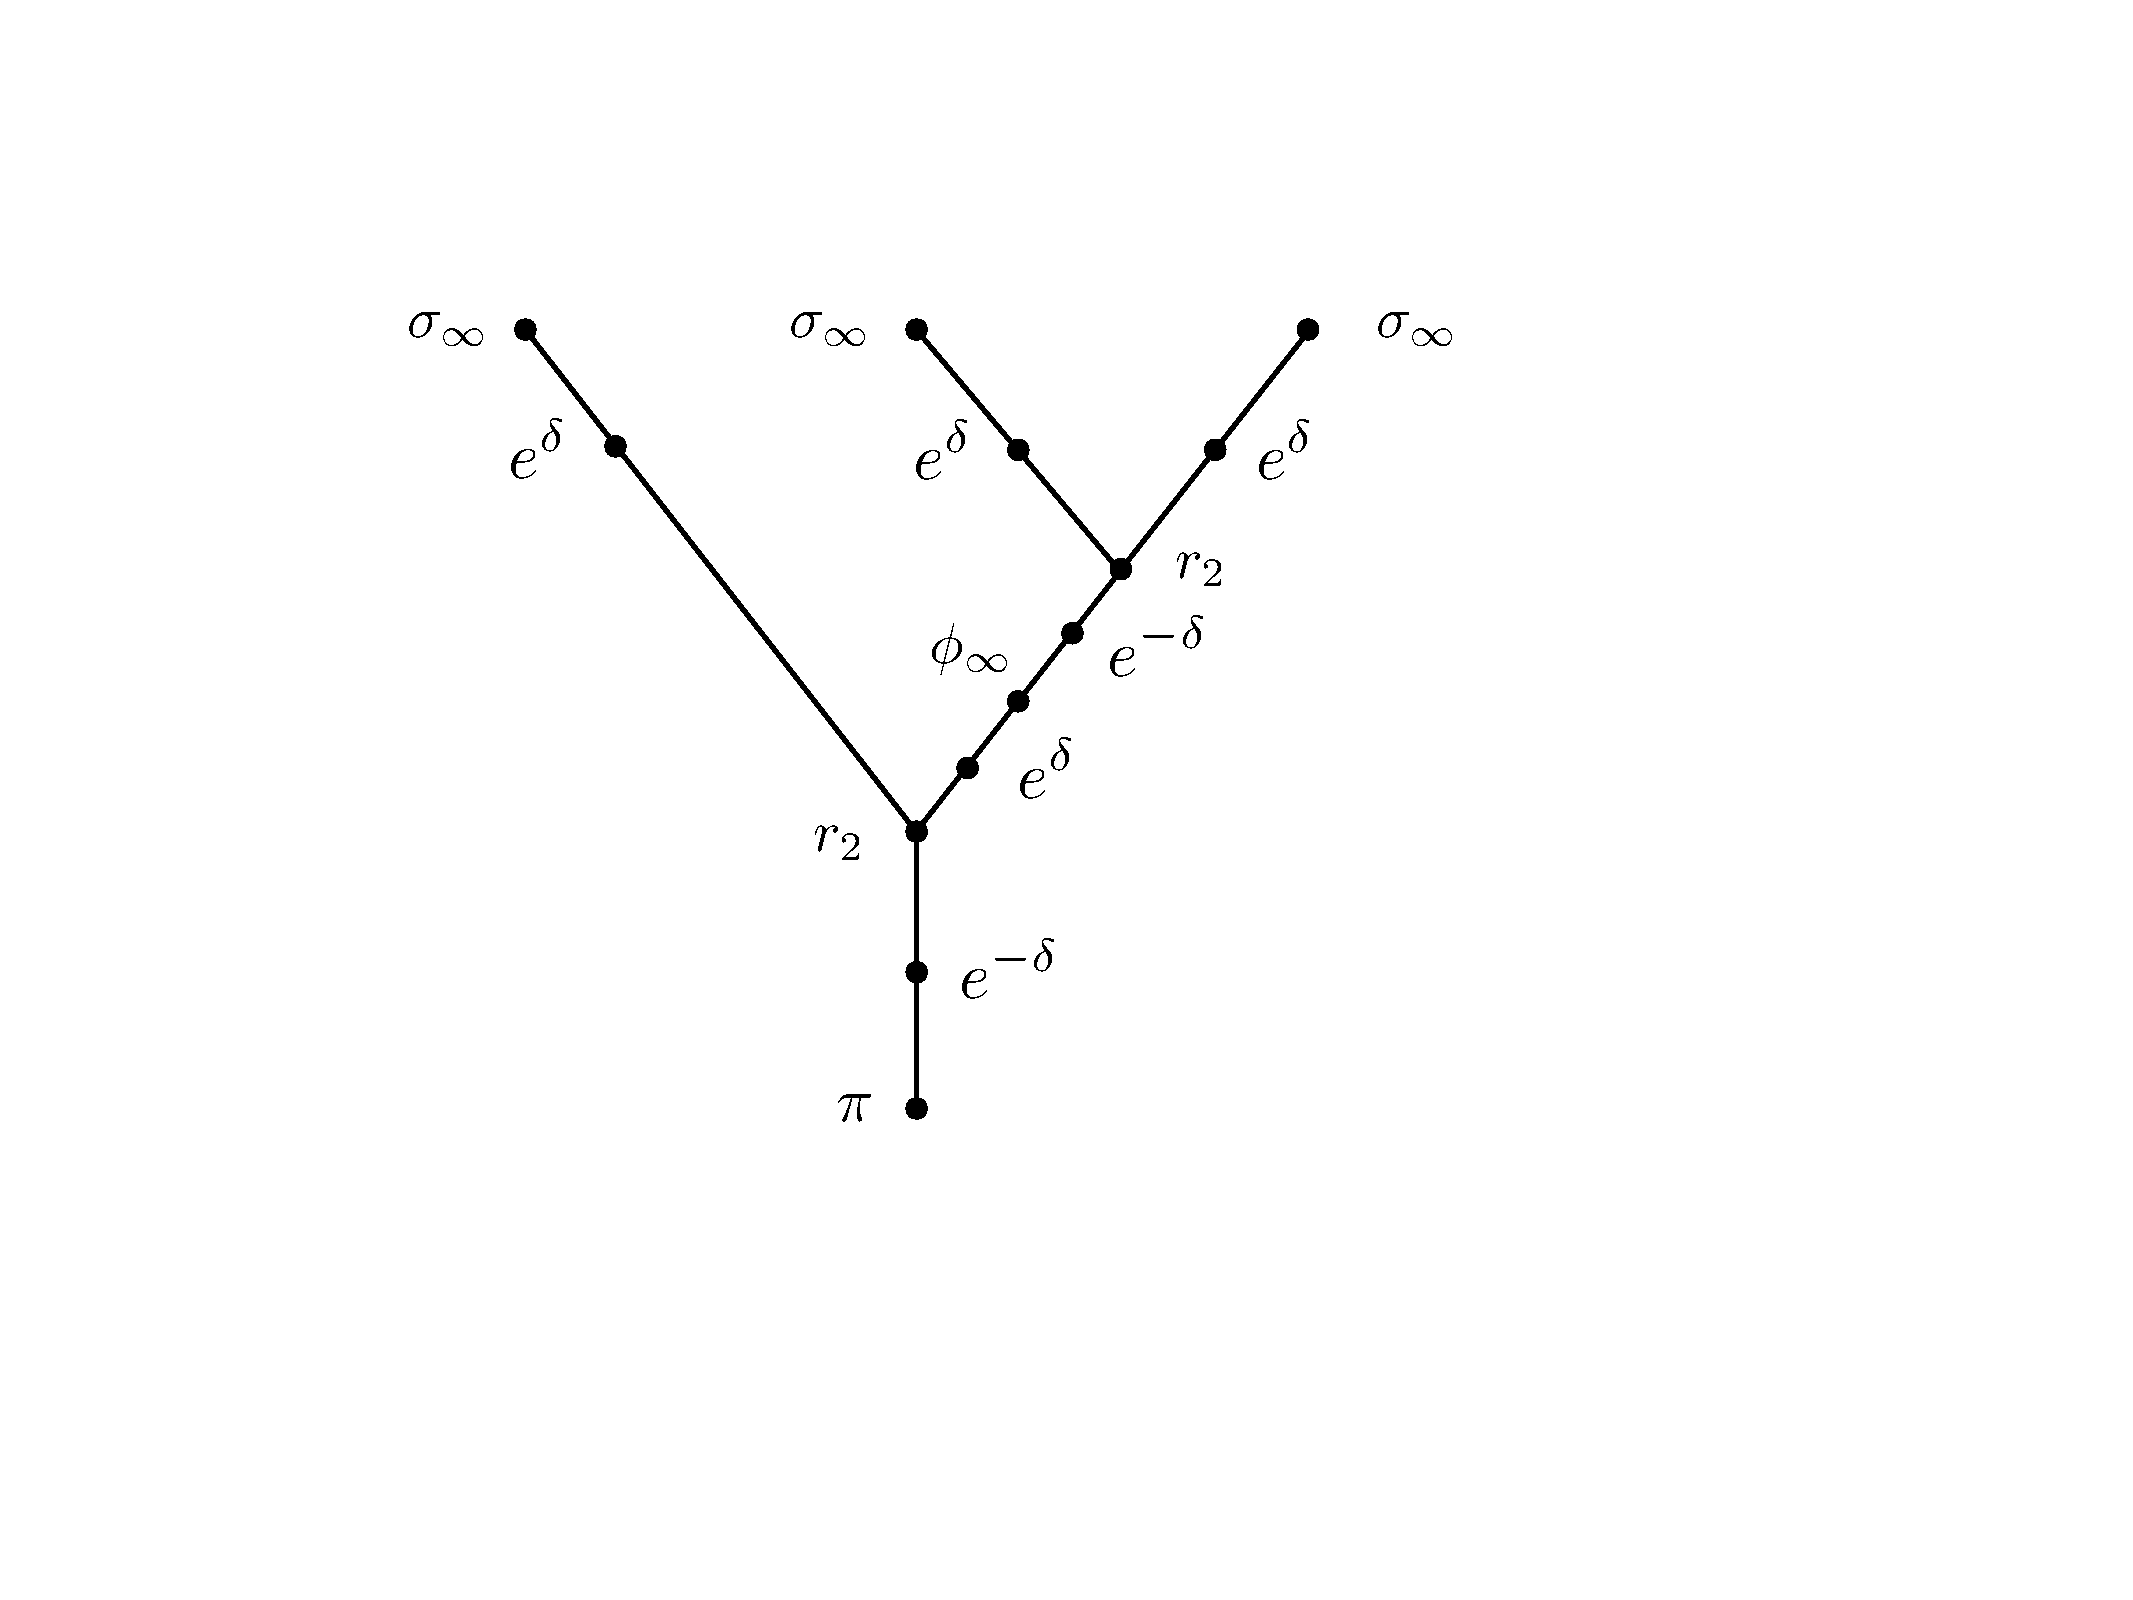
\includegraphics[scale=0.35]{dia13}
\end{center}
\centering
\caption{Example of an operator decorated tree.}\label{fig:opdectree}
\end{figure}
\be\label{eq:explicit_tree_operator}
- \pi e^{-\delta} r_2\Big( e^{\delta}\sigma_\infty \otimes e^{\delta} \phi_\infty e^{-\delta} r_2\Big( e^{\delta} \sigma_\infty \otimes e^{\delta} \sigma_\infty \Big) \Big)\,.
\ee
The sign arises from the fact that this tree has one internal edge. Evaluating such an operator on a tensor involves Koszul signs, arising from the $\nZ_2$-degree (with respect to the tilde grading) of the involved operators (recall that $r_2$ is odd).

We now have the notation to state the main theorem. Let $\cat{BT}_k$ denote the set of all plane trees with $k$ inputs (in the sense of Appendix \ref{??}). Note that all our $A_\infty$-categories, functors and homotopies are $k$-linear unless specified otherwise.

\begin{theorem}\label{theorem:main_ainfty_products} Define the odd $k$-linear map
\be\label{eq:rho_kintermsoftrees}
\rho_k = \sum_{T \in \cat{BT}_k} \rho_T : \HH_{\BB}[1]^{\otimes k} \lto \HH_{\BB}[1]
\ee
where for a binary tree $T$ with $k$ inputs, $\rho_T$ is $(-1)^{e_i(T)}$ times the denotation of the decoration which assigns $\HH_{\AA_\theta}$ to every leaf and $\HH_{\BB}$ to every edge, and
\begin{center}
%\begin{tabular}{ >{\centering}m{8cm} >{\centering}m{8cm}}
\begin{itemize}
\item \textbf{inputs:} $e^\delta \sigma_\infty$
\item \textbf{internal edges:} $e^\delta \phi_\infty e^{-\delta}$
\item \textbf{internal vertices:} $r_2$
\item \textbf{root:} $\pi e^{-\delta}$
\end{itemize}
%&
%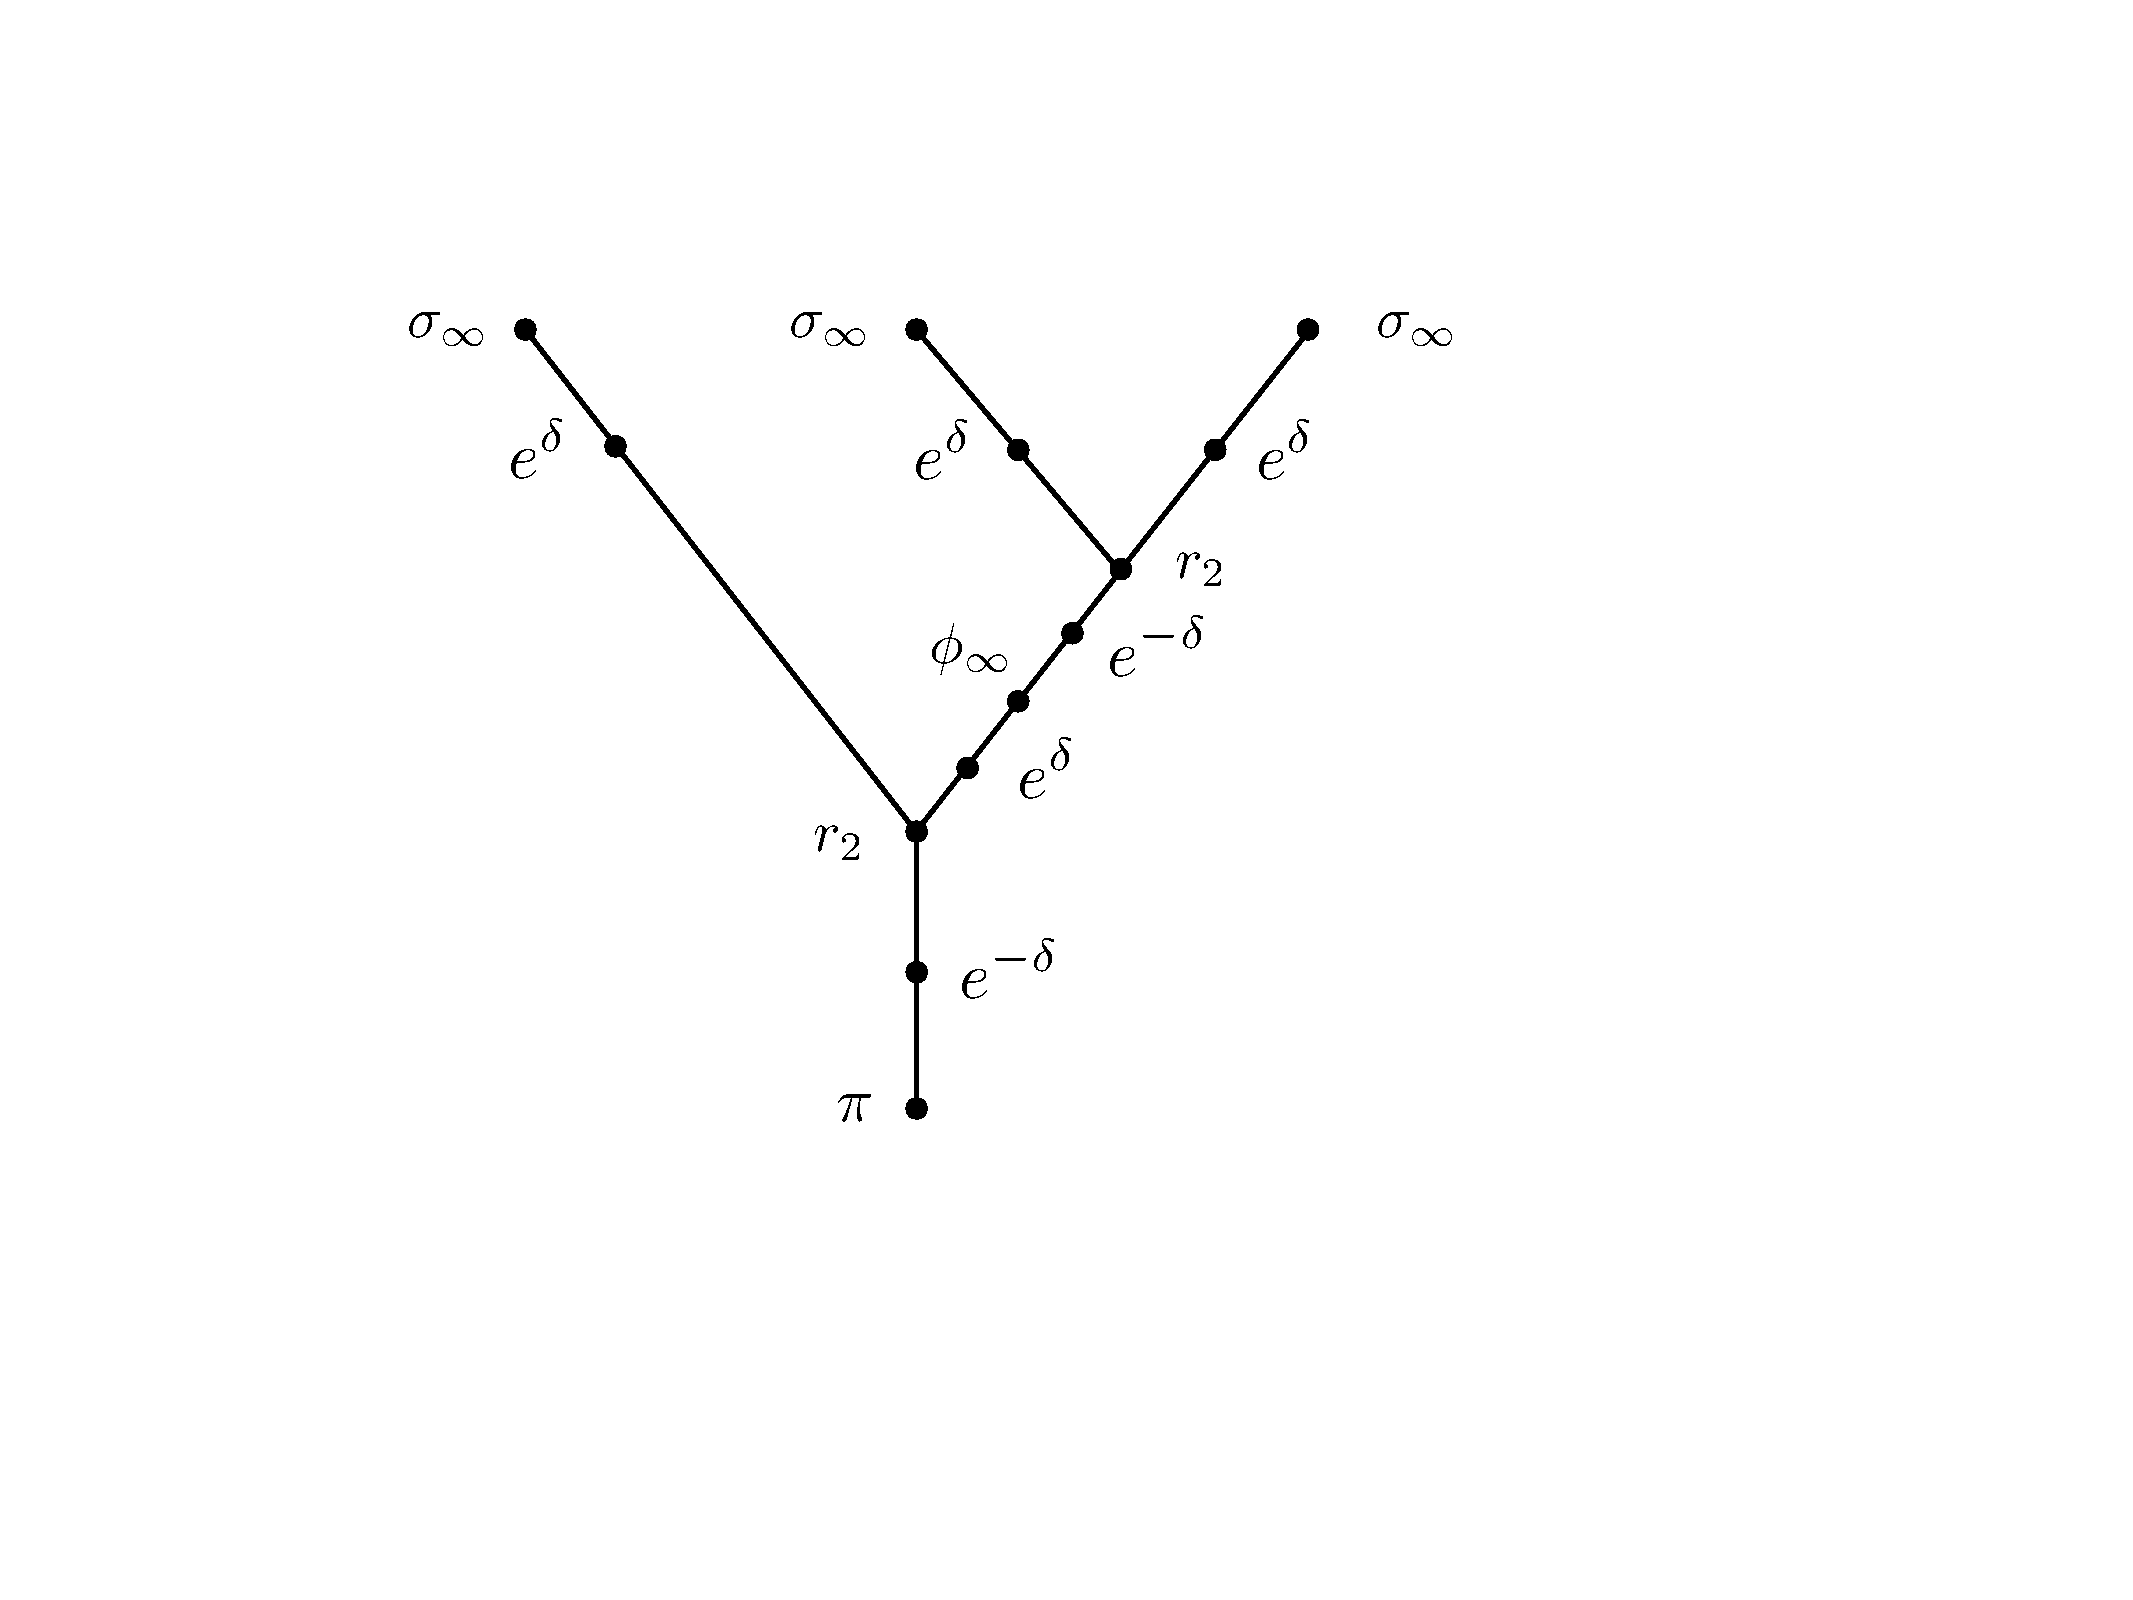
\includegraphics[scale=0.35]{dia13}
%\end{tabular}
\end{center}
Then $( \BB, \rho = \{ \rho_k \}_{k \ge 1} )$ is a strictly unital $A_\infty$-category and there are $A_\infty$-functors
\[
\xymatrix@C+3pc{
\AA_\theta \ar@<1ex>[r]^F & \BB \ar@<1ex>[l]^G
}
\]
and an $A_\infty$-homotopy $G \circ F \simeq 1_{\AA_{\theta}}$. %If $k$ is a field there is an $A_\infty$-homotopy $F \circ G \simeq 1_{\BB}$.
\end{theorem}
\begin{proof}
The full details are given in Appendix \ref{section:proofs}, but in short this is homological perturbation combined with Lemma \ref{lemma:completion_he}, applied to a particular choice of strong deformation retract arising from the connection $\nabla$ and the isomorphism $\exp(\delta)$.
\end{proof}

The projector $e$ of \eqref{eq:projector_e} can be written in terms of creation and annihilation operators
\[
e = \theta_n^* \cdots \theta_1^* \theta_1 \cdots \theta_n: \bigwedge F_\theta \lto \bigwedge F_\theta
\]
where $\theta_i$ denotes the operator $\theta_i \wedge (-)$ and $\theta_i^*$ denotes contraction $\theta_i^* \,\lrcorner\, (-)$. This is a morphism of algebras and induces a morphism of DG-algebras $e: \AA_\theta \lto \AA_\theta$.

\begin{definition} Let $E$ to be the following composite of $A_\infty$-functors 
\[
\xymatrix@C+2pc{
\BB \ar[r]^-G & \AA_\theta \ar[r]^-{e} & \AA_\theta \ar[r]^-F & \BB
}\,.
\]
\end{definition}

\begin{corollary}\label{corollary:idempotent_finite_model} The tuple $(\BB, \rho, E)$ is an idempotent finite model of $\AA \otimes_R \widehat{R}$.
\end{corollary}
\begin{proof}
Consider the diagram
\[
\xymatrix@C+3pc{
\AA \otimes_R \widehat{R} \ar@<1ex>[r]^-{i} & \AA_\theta \ar@<1ex>[l]^-{p} \ar@<1ex>[r]^F & \BB \ar@<1ex>[l]^G
}
\]
where $i$ is the natural inclusion and $p$ is the projection, so that $p \circ i = 1$ and $i \circ p = e$. These are both DG-functors. We define $I = F \circ i$ and $P = p \circ G$ as $A_\infty$-functors. Since we have an $A_\infty$-homotopy $G \circ F \simeq 1$ we have an $A_\infty$-homotopy
\[
P I = p G F i \simeq p i = 1
\]
and by definition $E = I \circ P$.
%\[
%EE = F e G F e G \simeq F e e G = FG = E\,.
%\]
\end{proof}

Recall that the purpose of the idempotent $E$ is that it encodes the information necessary to ``locate'' $\AA$ as a sub-$A_\infty$-algebra within the larger object $(\HH_{\BB}, \rho)$. The information in the lowest piece $E_1$ of this $A_\infty$-morphism is the most transparent, as it locates $\AA$ as a subcomplex within $\HH_{\BB}$. 

\begin{definition}\label{defn:gamma_anddagger} Let $\gamma_i$ be the $k$-linear cochain map
\[
\xymatrix@C+2pc{
\BB \ar[r]^-{G_1} & \AA_{\theta} \ar[r]^-{\theta_i^*} & \AA_{\theta} \ar[r]^-{F_1} & \BB
}
\]
and let $\gamma_i^\dagger$ be the $k$-linear cochain map
\[
\xymatrix@C+2pc{
\BB \ar[r]^-{G_1} & \AA_{\theta} \ar[r]^-{\theta_i} & \AA_{\theta} \ar[r]^-{F_1} & \BB
}
\]
\end{definition}

By definition there is a $k$-linear homotopy
\[
E_1 \simeq \gamma_n \cdots \gamma_1 \gamma_1^\dagger \cdots \gamma_n^\dagger\,.
\]
In \cite{cut} we computed explicit formulas for these operators on $\HH_{\BB}$ %, up to homotopy:

\begin{theorem}\label{theorem:homotopy_clifford} There are $k$-linear homotopies $\gamma_i \simeq \vAt_i$ and
\be
\gamma_i^\dagger \simeq -\lambda_i - \sum_{m \ge 1} \sum_{q_1,\ldots,q_m} \frac{1}{(m+1)!} \big[ \lambda_{q_m}\,, \big[ \lambda_{q_{m-1}}, \big[ \cdots [ \lambda_{q_1}, \lambda_i ] \cdots \big] \At_{q_1} \cdots \At_{q_m}\,.
\ee
\end{theorem}

As shown in \cite{pushforward} idempotent finite models $(\BB, \rho, E)$ expressed in terms of Atiyah classes are well-suited for understanding these categories (see e.g. the proof of the Hirzebruch-Riemann-Roch theorem for matrix factorisations in \cite{??}).

% In principle the passage from $(\HH_{\BB}, E)$ to a splitting should be easier to control, since the starting point is already finite, but we admittedly do not fully understand this problem. (TODO: we can strictify idempotents )

%If $k$ is a field we can pass to cohomology, split $E_1$ by taking  ; the details will appear in the sequel \cite{??}. 

%\begin{remark}
%When $k$ is a field the construction of $(R/I \otimes_R \AA, \{ \rho_k \}_{k \ge 1}, E)$ is an \emph{algorithm} in the following precise sense. Once we choose a sequence of MFs $X_0,\ldots,X_k$ together with homogeneous bases for each, homotopies $\lambda_i$ and a Gr\"obner basis for $I$, we can use the Euclidean division algorithm to define the section $\sigma$, the connection $\nabla$ and a $k$-basis of monomials for $R/I$ (see Remark \ref{remark:grobner}). With respect to these choices, $\rho_k$ is a matrix with entries in $k$.

%As we will make explicit in Section \ref{??} with $k$ fixed the Feynman diagrams that contribute to the calculation of $\rho_k$ only involve \emph{polynomials} in $t$ of degree $\le k - 2$ and the operators that arise from inverting $\sigma_{\bold{t}}$ on polynomials appearing in the differentials of the $X_i$ and the $\lambda_i$ may be computed in these $t$-degrees by the algorithm of Remark \ref{remark:grobner}. Similarly $\Gamma$ (TODO).

%However for general $k$ there is a nonconstructive element, which is the choice of $a_i$ (cite generic Gr\"obner bases).
%\end{remark}

%\begin{remark}
%In the case where $k$ is a field, let us sketch how a \emph{minimal} model can be obtained from the idempotent finite model; details will appear elsewhere. We can simply apply the usual minimal model construction to $(R/I \otimes_R \AA, \{ \rho_k \}_{k \ge 1})$ keeping in mind that this $A_\infty$-category is locally finite-dimensional, so that the choices involved in performing the minimal model construction are finite. In any case, we get a homotopy equivalence to
%\[
%( H^*( R/I \otimes_R \AA ), \tau, E' )
%\]
%with an idempotent self $A_\infty$-morphism $E'$, all the structures in which are determined in terms of those finite choices. Then $E'_1$ is a strict idempotent linear operator, and we may set $B = Im(E'_1)$. By solving a series of recursive equations we can determine an $A_\infty$-structure $\kappa$ on $B$ and morphisms of $A_\infty$-algebras
%\[
%\xymatrix@C+1pc{
%( H^*( R/I \otimes_R \AA ), \tau ) \ar@<1ex>[r]^-f & ( B, \bold{\kappa} ) \ar@<1ex>[l]^-g
%}
%\]
%with $f \circ g \simeq 1_B, g \circ f \simeq E'$. Then $(B, \kappa)$ is an $A_\infty$-minimal model of $\AA$. 
%\end{remark}

As explained in the introduction, the idea of the idempotent finite model of $\AA$ is that it is both finite over $k$ \emph{and} its structure is related in a controlled way to that of $\AA$. We can be more precise:

\begin{remark}
The idempotent finite model of Theorem \ref{??} is constructive, at least when $k$ is a field. To explain, note that for a fixed integer $k$ and sequence of matrix factorisations $X_0,\ldots,X_k$ we have linear maps
\[
\rho_k: \bigotimes_{i=n}^1 \Big[ R/I \otimes \Hom_k(\widetilde{X}_{i-1}, \widetilde{X}_i) \Big][1] \lto \big[ R/I \otimes \Hom_k( \widetilde{X}_1, \widetilde{X}_0 ) \big][1]\,.
\]
Choose bases for $R/I$ and the involved matrix factorisations (for $R/I$ this can be done using Gr\"obner bases). Then $\rho_k$ is determined by a matrix $[ \rho_k ]$, and we give an algorithm to calculate the entries in this matrix: that is what we mean when we say that the $A_\infty$-structure on $\BB$ is constructive.

Indeed, in this paper our focus is on giving a Feynman diagram presentation of the higher operations $\rho_k$, with an emphasis on how the local interactions that generate these diagrams are obtained from the Atiyah class $\vAt$ and the chosen homotopies. A similar presentation applies to $\varphi, \psi$ and $E$ using the formulas of \cite{markl_transfer}, and this will be given in the sequel \cite{??}.
\end{remark}

\begin{remark}\label{remark:on_generator}
It is natural to ask if $E$ can be split within Hom-finite $A_\infty$-categories, in a ``controlled'' way, but unfortunately we only have a partial understanding of this problem in general. However it is worth noting that if $\AA$ consists of the single object $k^{\stab}$ with $\bold{t} = (x_1,\ldots,x_n)$, it is easy to split $E_1$ by computing
\[
\bigcap_{i=1}^n \Ker(\gamma_i)
\]
and this subspace turn out to be closed under the higher operations on $\BB$, so that $\operatorname{Im}(E_1)$ with the restricted operators is a splitting of $E$ as an $A_\infty$-functor (details will appear in \cite{??}). This leads to a minimal model of $\AA(k^{\stab}, k^{\stab})$ related to the standard one \cite{??,??,??}.
\end{remark}
%It is natural to ask if we can \emph{split} the idempotent $E$ in some controlled way within $A_\infty$-algebras Hom-finite over $k$, and in this way obtain a finite $A_\infty$-algebra directly quasi-isomorphic to $\AA$. If $k$ is a field we can certainly split $E$, since $H^*(\AA)$ is Hom-finite and any minimal model gives rise to a splitting. However, the point is that without a good choice of cohomological splitting this is hard to make constructive in a useful way.
% 

\textbf{Outline of the paper.} There are several factors which complicate actual calculations with such decorated trees:
\begin{itemize}
\item Many of the involved operators (e.g. the $\lambda_i$ and $D$) involve multiplications by polynomials which we must evaluate by transfer to $R/I \otimes k\llbracket \bold{t} \rrbracket$. We explain how to think about such operations in terms of contraction with a tensor $\Gamma$ in Section \ref{??}.
\item At each internal vertex we have the forward suspended composition $r_2$ which introduces complicated signs; for reasoning about such trees by hand, it is better to extract a global sign for each tree and work with the usual composition in $\AA$, as we explain in Section \ref{??}.
\item The factors $\zeta$ introduce scalar factors that require further analysis.

\item Finally, to understand the large composition (contraction) of operators that $\langle D \rangle$ represents, it is helpful to view it as a large composition of creation and annihilation operators and apply Feynman diagrams to organise the resulting sums, which we explain in Section \ref{??}. %Finally, in good cases like the standard generator $k^{\stab}$ we can make an even more simplified presentation by cancelling many of the $e^{\delta}, e^{-\delta}$ operators, as we explain in Section \ref{??}.
\end{itemize}

\section{Towards Feynman diagrams}

We have given a definition of the forward suspended $A_\infty$-products on $\BB$. However, it is hard to reason about these products without further teasing out the interaction vertices underlying the exponentials in \eqref{??} and switching from the forward suspended composition $r_2$ to the ordinary composition $\mu_2$. In this section we learn how to write the $\rho_T$ in terms of simple contractions of tensors associated to edges of the tree $T$, which we can in turn interpret as vertices in Feynman diagrams as suggested in the introduction.

Throughout this section the conventions of Setup \ref{setup:overall} remain in force. Given a binary tree $T$ we denote by $T'$ the \emph{mirror} of $T$, which is obtained by exchanging the left and right branch at every vertex. Given a binary tree $T$ decorated as explained in Theorem \ref{??} let $\operatorname{eval}_T$ be the operator obtained by evaluating the tree without Koszul signs.

%On the one hand, the forward suspended multiplication $r_2$ involves awkward signs that complicate a diagrammatic presentation, so it is better to switch to the ordinary multiplication $\mu_2$. Moreover, at the moment the Feynman rules involve operators on the completion $\widehat{R}$ which is a complicated object. However, we know from Theorem \ref{prop_algtube} how to rewrite this in terms of simpler objects. 

\begin{lemma}\label{prop:replacer2} We have
\be\label{eq:proprhoT}
\rho_T( \xi_1, \ldots, \xi_k ) = (-1)^{e_i(T) + \sum_{i < j} \widetilde{\xi}_i \widetilde{\xi}_j + \sum_i \widetilde{\xi}_i P_i + k + 1} \operatorname{eval}_{T'}( \xi_k, \ldots, \xi_1 )\,.
\ee
where $P_i$ is the number of times the path from the $i$th leaf in $T$ (counting from the left) enters a trivalent vertex as the right-hand branch on its way to the root, and $k+1$ is the number of internal vertices in $T$.
\end{lemma}
\begin{proof}
Let us begin with the special case given in Figure \ref{fig:opdectree}, using
\be\label{eq:mu2vsr2_v2}
r_2( \xi_1, \xi_2 ) = (-1)^{\widetilde{\xi_1} \widetilde{\xi_2} + \widetilde{\xi_2} + 1}
\mu_2(\xi_2 \otimes \xi_1)
\ee
and the operator given in \eqref{eq:explicit_tree_operator} to compute that
\begin{align*}
\rho_T( \xi_1, \xi_2, \xi_3 ) &= (-1)^{e_i(T)} \pi e^{-\delta} r_2\Big( e^{\delta}\sigma_\infty \otimes e^{\delta} \phi_\infty e^{-\delta} r_2\Big( e^{\delta} \sigma_\infty \otimes e^{\delta} \sigma_\infty \Big) \Big)( \xi_1 \otimes \xi_2 \otimes \xi_3 )\\
&= (-1)^{e_i(T) + a} \pi e^{-\delta} r_2\Big( e^{\delta}\sigma_\infty(\xi_1) \otimes e^{\delta} \phi_\infty e^{-\delta} r_2\Big( e^{\delta} \sigma_\infty(\xi_2) \otimes e^{\delta} \sigma_\infty(\xi_3) \Big) \Big)
\end{align*}
where $a = \widetilde{\xi_1}( |\phi_\infty| + |r_2| ) \equiv 0$ gives the Koszul sign arising from moving the inputs ``into position''. Note that since $|\delta| = |\sigma_\infty| = 0$ and every $r_2$ on the tree $T$, except for the one adjacent to the root, is followed immediately by a $\phi_\infty$, this Koszul sign is always $+1$.

Hence the signs that arise in computing $\rho_T(\xi_1,\ldots,\xi_k)$ in terms of $\mu_2$ on the mirrored tree arise entirely from \eqref{eq:mu2vsr2_v2}. If we continue to calculate, we find
\begin{align*}
&= (-1)^{e_i(T) + b} \pi e^{-\delta} \mu_2\Big( e^{\delta} \phi_\infty e^{-\delta} r_2\Big( e^{\delta} \sigma_\infty(\xi_2) \otimes e^{\delta} \sigma_\infty(\xi_3) \Big) \otimes e^{\delta}\sigma_\infty(\xi_1) \Big)\\
&= (-1)^{e_i(T) + b + c} \pi e^{-\delta} \mu_2\Big( e^{\delta} \phi_\infty e^{-\delta} \mu_2\Big( e^{\delta} \sigma_\infty(\xi_3) \otimes e^{\delta} \sigma_\infty(\xi_2) \Big) \otimes e^{\delta}\sigma_\infty(\xi_1) \Big)\\
&= (-1)^{e_i(T) + b + c} \operatorname{eval}_{T'}( \xi_3, \xi_2, \xi_1 )
\end{align*}
where
\[
b = \widetilde{\xi_1}( \widetilde{\xi_2} + \widetilde{\xi_3} ) + \widetilde{\xi_2} + \widetilde{\xi_3} + 1\,, \qquad c = \widetilde{\xi_2}\widetilde{\xi_3} + \widetilde{\xi_3} + 1\,.
\]
This verifies the sign in the special case, where $P_1 = 0, P_2 = 1, P_3 = 2$. By induction on the height of tree, it is easy to check that in general there is a contribution to the sign of a $\widetilde{\xi_i}\widetilde{\xi_j}$ at the vertex where the path from the $i$th and $j$th leaves to the root meet for the first time, and a $\widetilde{\xi_i}$ every time the path from the $i$th leaf enters a trivalent vertex on the right branch (of $T$), as claimed.
\end{proof}

\subsection{Transfer to $R/I \otimes k\llbracket \bold{t} \rrbracket$}

Recall that given a choice of section $\sigma: R/I \lto R$, which we have fixed above in Setup \ref{setup:overall}, there is by Lemma \ref{prop_algtube} an associated $k\llbracket \bold{t} \rrbracket$-linear isomorphism
\[
\sigmastar: R/I \otimes k \llbracket \bold{t} \rrbracket \lto \widehat{R}\,.
\]
From this we obtain \eqref{eq:transfer_iso_intro} which is used to transfer operators on $\Hom_R(Y,X) \otimes_R \widehat{R}$ (such as the differential or the homotopies $\lambda$) to operators on $R/I \otimes \Hom_k(\widetilde{Y}, \widetilde{X}) \otimes k\llbracket \bold{t} \rrbracket$. Since this introduces various complexities we should first justify why such transfers are necessary: that is, why do we prefer the left hand side of \eqref{eq:transfer_iso_intro} to the right hand side?

Recall that the higher products $\rho_k$ on $\HH_{\BB}$ are defined in terms of operators on the larger space $\HH_{\AA_\theta}$. If we are to reason about these higher products using Feynman diagrams, then to the extent that it is possible, the operators involved should be written as polynomials in creation and annihilation operators for either bosonic or fermionic Fock spaces (that is, in terms of multiplication by or the derivative with respect to ordinary polynomial variables $t$ or odd Grassmann variables $\theta$). It is not obvious \emph{a priori} how to do this: recall that in order to ensure that the connection $\nabla$ existed we had to pass from $R = k[x_1,\ldots,x_n]$ to the $I$-adic completion $\widehat{R}$, which in general is not a power series ring. For example, it is not clear how to express the operation of multiplication by $r \in R$, which we denote by $r^{\#}$, in terms of creation and annihilation operators on $\Hom_R(Y,X) \otimes_R \widehat{R}$.

The purpose of this section is then to explain how the isomorphism $\sigma_{\bold{t}}$ is the canonical means by which to express $r^{\#}$ in terms of creation operators for ``bosonic'' degrees of freedom, here represented by polynomials in the $t_i$.
\\

In what follows we fix a chosen $k$-basis of $R/I$, which we denote
\[
R/I = k z_1 \oplus \cdots \oplus k z_\mu\,.
\]
When $k$ is a field there is a natural monomial basis for $R/I$ associated to any choice of a monomial ordering on $k[x_1,\ldots,x_n]$ and Gr\"obner basis for $I$, see Remark \ref{remark:grobner}. Since $\sigmastar$ is not, in general, an algebra isomorphism (see Lemma \ref{prop_algtube}) there is information in the transfer of the multiplicative structure on $\widehat{R}$ to an operator on $R/I \otimes k\llbracket \bold{t} \rrbracket$, and we record this information in the following tensor:

\begin{definition}\label{defn_gamma} Let $\Gamma$ denote the $k$-linear map
\[
\xymatrix@C+2pc{
R/I \otimes R/I \ar[r]^-{ \sigma \otimes \sigma } & \widehat{R} \otimes \widehat{R} \ar[r]^-{m} & \widehat{R} \ar[r]^-{(\sigmastar)^{-1}} & R/I \otimes k\llbracket \bold{t} \rrbracket
}
\]
where $m$ denotes the usual multiplication on $\widehat{R}$. We define $\Gamma$ as a tensor via the formula
\[
\sigma(z_i)\sigma(z_j) = \sum_{k=1}^\mu \sum_{\delta \in \mathbb{N}^n} \Gamma^{ij}_{k \delta} \sigma(z_k) t^\delta\,.
\]
\end{definition}

\begin{definition}\label{defn:rsharp} Given $r \in R$ we write $r_{(i,\delta)}$ for the unique collection of coefficients in $k$ with the property that in $\widehat{R}$ there is an equality
\[
r = \sum_{i = 1}^\mu \sum_{\delta \in \mathbb{N}^n} r_{(i,\delta)} \,\sigma(z_i) t^{\delta}\,.
\]
Given $r \in R$ we denote by $r^{\#}$ the $k\llbracket \bold{t} \rrbracket$-linear operator
\[
\xymatrix@C+2pc{
R/I \otimes k\llbracket \bold{t} \rrbracket \ar[r]^-{\sigmastar} & \widehat{R} \ar[r]^{r} & \widehat{R} \ar[r]^-{(\sigmastar)^{-1}} & R/I \otimes k\llbracket \bold{t} \rrbracket
}
\]
where $r: \widehat{R} \lto \widehat{R}$ denotes multiplication by $r$.
\end{definition}

\begin{remark} For the overall construction of the idempotent finite model to be \emph{constructive} in the sense elaborated above, it is crucial that we have an algorithm for computing these coefficients $r_{(i, \delta)}$. In the notation of Section \ref{section:formaltub}, $r_{(i, \delta)}$ is precisely the coefficient of $z_i$ in the vector $r_\delta \in R/I$, so it suffices to understand how to compute the $r_\delta$.

As a trivial example, if $\bold{t} = (x_1,\ldots,x_n)$ then $R/I = k$ so $\mu = 1$ and $r_{(1,\delta)}$ is just the coefficient of the monomial $t^{\delta} = x^{\delta}$ in the polynomial $r$. In general, when $k$ is a field there is an algorithm for computing $r_\delta$ by iterated Euclidean division; see Remark \ref{remark:grobner}.
\end{remark}

\begin{lemma}\label{lemma:rsharp_explicit} The operator $r^{\#}$ is given in terms of the tensor $\Gamma$ by the formula
\be
r^{\#}(z_i) = \sum_{l=1}^\mu \sum_{\delta \in \mathbb{N}^n} \Big[ \sum_{\alpha + \beta = \delta } \sum_{k=1}^\mu r_{(k,\alpha)} \Gamma^{ki}_{l\beta} \Big] z_l \otimes t^\delta\,.
\ee
\end{lemma}
\begin{proof}
We have
\begin{align*}
\sigmastar r^{\#}(z_i \otimes 1) &= r \sigma(z_i)\\
&= \sum_{k, \alpha} r_{(k,\alpha)} [ \sigma(z_k) \sigma(z_i) ] t^{\alpha}\\
&= \sum_{k,\alpha,l,\beta} r_{(k,\alpha)} \Gamma^{ki}_{l \beta} \sigma(z_l) t^{\alpha + \beta}\\
&= \sum_\delta \sum_{k,l} \sum_{\alpha + \beta = \delta} r_{(k,\alpha)} \Gamma^{ki}_{l \beta} \sigma(z_l)t^\delta
\end{align*}
as claimed.
\end{proof}

\subsection{Propagators}\label{section:propagator}

One of the most complex aspects of calculating the $A_\infty$-products described by Theorem \ref{theorem:main_ainfty_products} are the scalar factors contributed by the operator $\zeta$ which is the inverse of the grading operator for the virtual degree. In this section we provide a closer analysis of these factors.

\begin{definition} We define the \emph{virtual degree} of a tensor $\omega \otimes z_i \otimes \alpha \otimes t^{\tau} \in \HH$ to be $|\omega| + |\tau|$.
\end{definition}

The virtual degree is genuinely a $\nZ$-grading and not a $\nZ_2$-grading. Observe that that the critical Atiyah class $\vAt = [ \nabla, d_{\AA} ]$ is not homogeneous with respect to this grading, because while $\nabla$ is homogeneous of degree zero with respect to the virtual degree (since $\theta_i$ has virtual degree $+1$ and $\partial_{t_i}$ has virtual degree $-1$) the operator $d_{\AA}$ involves multiplications by polynomials $r$ which need not have a consistent degree (viewed as operators $r^{\#}$ on $R/I \otimes k\llbracket \bold{t} \rrbracket$ as in \eqref{??}). A product of operators of the form
\[
(\zeta \vAt)^m = \zeta \vAt \zeta \vAt \cdots \zeta \vAt
\]
can be expressed as a matrix of operators on $\bigwedge F_\theta \otimes R/I \otimes k \llbracket \bold{t} \rrbracket$ of the form
\begin{align*}
\zeta [ \nabla, r_m^{\#} ] \cdots \zeta [ \nabla, r_1^{\#} ] &= \sum_{i_1,\ldots,i_m} \zeta \theta_{i_m} [ \partial_{t_{i_m}}, r_m^{\#} ] \zeta \cdots \zeta \theta_{i_1} [ \partial_{t_{i_1}}, r_1^{\#} ]
\end{align*}
We may write $r^{\#} = \sum_{\delta \in \mathbb{N}^m} r[\delta] t^\delta$ for some operator $r[\delta]$, a formula for which can be inferred from Lemma \ref{lemma:rsharp_explicit} but which we will not need. Using this
\begin{align*}
(\zeta \vAt)^m &= \sum_{i_1,\ldots,i_m} \sum_{\delta_1, \ldots, \delta_m} \zeta \theta_{i_m} r_m[\delta_m] \partial_{t_{i_m}}(t^{\delta_m}) \zeta \cdots \zeta \theta_{i_1} r_1[\delta_1] \partial_{t_{i_1}}(t^{\delta_1})
\end{align*}
(TODO: relate to later A-types) Evaluated on a tensor $\omega$ of homogeneous virtual degree this gives
\begin{align*}
(\zeta \vAt)^m(\omega) &= \sum_{i_1, \ldots, i_m} \sum_{\delta_1,\ldots,\delta_m} Z(|\omega|,|\delta_1|,\ldots,|\delta_m|) \cdot \theta_{i_m} r_m[\delta_m] \partial_{t_{i_m}}(t^{\delta_m}) \cdots \theta_{i_1} r_1[\delta_1] \partial_{t_{i_1}}(t^{\delta_1})(\omega)
\end{align*}
where the scalar factor is computed by
\[
Z^{\,\rightarrow}(a,d_1,\ldots,d_m) = \frac{1}{a + d_1} \frac{1}{a + d_1 + d_{2}} \cdots \frac{1}{a + d_1 + \cdots + d_m}\,.
\]
Only sequences of distinct $\theta$'s contribute to the sum, so $(\zeta \vAt)^m(\omega)$ equals
\begin{align*}
\sum_{i_1 < \cdots < i_m} \sum_{\delta_1,\ldots,\delta_m} Z(|\omega|,|\delta_{\sigma(1)}|,\ldots,|\delta_{\sigma(m)}|) \cdot \prod_{j=1}^m r_{m+1-j}[\delta_{m+1-j}] \cdot t^{\sum_j \delta_j - \bold{e}_{i_1} - \cdots - \bold{e}_{i_m}} \theta_{\bold{i}}\; \omega
\end{align*}
where $\theta_{\bold{i}} = \theta_{i_m} \cdots \theta_{i_1}$, the product of $r[\delta]$ operators is expanded from left to right as the index $j$ increases, and we use the notation of the next definition.

\begin{definition} Given integers $a > 0$ and a sequence $d_1, \ldots, d_m \in \mathbb{N}$ we define
\begin{align*}
Z(a,d_1,\ldots,d_m) &= \sum_{\sigma \in S_m} Z^{\,\rightarrow}(a,d_{\sigma(1)},\ldots,d_{\sigma(m)})\\
&= \sum_{\sigma \in S_m} \frac{1}{a + d_{\sigma(1)}} \frac{1}{a + d_{\sigma(1)} + d_{\sigma(2)}} \cdots \frac{1}{a + d_{\sigma(1)} + \cdots + d_{\sigma(m)}}\,.
\end{align*}
\end{definition}

Why can we ignore signs $(-1)^{|\sigma|}$ here?

Such scalar factors are a common occurrence in QFT, and are usually discussed in the context of infrared divergences involving soft virtual particles (such as soft virtual photons in quantum electrodynamics) see for instance \cite[Ch. 13]{weinberg} and \cite[p.204]{ps}. The most commonly treated case in textbooks is the case of an on-shell external electron line, which corresponds to taking $a = 0$. It is easy to see in this case that there is a simple formula for $Z$:

\begin{lemma} Given a sequence $d_1,\ldots,d_m \ge 1$ of integers,
\be
Z(0,d_1,\ldots,d_m) = \sum_{\sigma \in S_m} \frac{1}{d_{\sigma(1)}} \frac{1}{d_{\sigma(1)} + d_{\sigma(2)}} \cdots \frac{1}{d_{\sigma(1)} + \cdots + d_{\sigma(m)}} = \frac{1}{d_1 \cdots d_m}\,.
\ee
\end{lemma}

However, we do not know any simple form of $Z$ in general. The factors contributed by $\zeta$ are just propagators, similar to $\frac{1}{p^2 - m^2 + i \varepsilon}$ with suppress contributions from off the mass-shell (the further off the mass-shell you are, the larger $p^2-m^2$ is). In our case, Feynman diagrams with large numbers of internal virtual particle lines ($\theta$ and $t$ states) are generically suppressed (with respect to the usual metric on $\mathbb{Q}$).

\section{Feynman diagrams}\label{section:feynman_diagram}
% REF: (ainfmf30)

There is a presentation of the $A_\infty$-products on $\BB$ in terms of Feynman diagrams, which is particularly satisfactory when the objects $\AA$ are all matrix factorisations of Koszul type. The purpose of Feynman diagrams in Quantum Field Theory is twofold: they give an algorithmic method for computing scattering amplitudes (to some approximation) and they are also a \emph{tool for reasoning} about physical processes. The intended role of Feynman diagrams here is similar: they provide both an algorithmic method for computing higher $A_\infty$-products, and a tool for reasoning about these products.\footnote{Of course, there is no free lunch: as in QFT, the diagrams and associated calculations may be \emph{very} complicated and infeasible to do by hand except in the simplest examples.} The presentation of $A_\infty$-structures in terms of Feynman diagrams is an old idea going back to Kontsevich \cite{??} see also \cite{??}. As references for Feynman diagrams in physics we recommend \cite[Ch. 6]{weinberg}, \cite[\S 4.4]{ps}, while a more mathematical treatment can be found in \cite{qftstring}. However, we will assume the reader has no prior exposure to Feynman diagrams in the following.

Throughout we adopt the hypotheses of Setup \ref{setup:overall}, and we write
\be\label{eq:hhalt_koszul}
\HH = \HH_{\AA'_\theta}\,, \qquad \HH(X,Y) = \bigwedge F_\theta \otimes R/I \otimes \Hom_k(\widetilde{X},\widetilde{Y}) \otimes k\llbracket \bold{t} \rrbracket\,.
\ee
Our aim is understand operators of the form \eqref{eq:explicit_tree_operator} in terms of Feynman diagrams. Implicitly this particular operator consists of many summands, obtained by expanding the $e^{\delta}, e^{-\delta}$ and $\sigma_\infty, \phi_\infty$ operators. Among the summands thus generated is for example
\be\label{eq:contrib_feynman}
\pi \delta^2 r_2\Big( (\zeta \vAt)^2 \sigma \otimes \delta^3 (\zeta \vAt)^3 \zeta \nabla \delta r_2\Big( \delta^5 (\zeta \vAt)^6 \sigma \otimes (\zeta \vAt) \sigma \Big) \Big)\,.
\ee
The aim is to
\begin{itemize}
\item represent the space $\HH$ on which these operators act as a tensor product of exterior algebras and (completed) symmetric algebras, and
\item represent the operators as polynomials in creation and annihilation operators (that is, as multiplication with, or the derivative with respect to, even or odd generators of the relevant algebras).
\end{itemize}
Once this is done we can represent the operator \eqref{eq:contrib_feynman} as the contraction of a set of polynomials in creation and annihilation operators, with the pattern of contractions dictated by the structure of the original tree. The process of \emph{reducing this contraction to normal form} (with all annihilation operators on the right, and creation operators on the left) involves commuting creation and annihilation operators past one another, and their commutation relations generate many new terms. Feynman diagrams provide a calculus for organising these terms, and thus computing the normal form.

There are three classes of operators making up \eqref{eq:contrib_feynman} which need to be given a diagrammatic interpretation:
\begin{itemize}
\item In Section \ref{section:koszul_mf} we represent $\HH$ as suggested above.
\item In Section \ref{section:fenyman_diagram_1} we treat $\vAt, \delta$.
\item In Section \ref{section:fenyman_diagram_2} we treat $\zeta$.
\item In Section \ref{section:feynman_diagram_3} we treat $r_2$.
\end{itemize}
Finally, in Section \ref{section:feynman_diagram_4} this is all brought together and demonstrated in an example.

\subsection{Koszul matrix factorisations}\label{section:koszul_mf}

Our Feynman diagrams will have vertices representing certain operators on $\HH(X,Y)$ for a pair of matrix factorisations $X,Y$ of $W$ of Koszul type \cite{??}. This means that we suppose given collections of polynomials $\{ f_i, g_i \}_{i=1}^r$ and $\{ u_j, v_j \}_{j=1}^s$ in $R$ satisfying
\[
W = \sum_{i=1}^r f_i g_i = \sum_{j=1}^s u_j v_j\,.
\]
To these polynomials we may associate matrix factorisations $X,Y$ defined as follows: we take odd generators $\xi_1,\ldots,\xi_r,\eta_1,\ldots,\eta_s$, set $F_\xi = \bigoplus_{i=1}^r k \xi_i, F_\eta = \bigoplus_{j=1}^s k \eta_j$ and
\begin{align}
\widetilde{X} &= \bigwedge F_\xi = \bigwedge( k \xi_1 \oplus \cdots \oplus k \xi_r )\label{eq:defn_X_tilde}\\
\widetilde{Y} &= \bigwedge F_\eta = \bigwedge( k \eta_1 \oplus \cdots \oplus k \eta_s )\label{eq:defn_Y_tilde}
\end{align}
and then define
\begin{align*}
X &= \big( \widetilde{X} \otimes R, \sum_{i=1}^r f_i \xi_i^* + \sum_{i=1}^r g_i \xi_i \big)\,,\\
Y &= \big( \widetilde{Y} \otimes R, \sum_{j=1}^s u_j \eta_j^* + \sum_{j=1}^s v_j \eta_j \big)\,.
\end{align*}
We ultimately want to give a graphical representation of operators on the $k$-module \eqref{eq:hhalt_koszul}, for which relevant operators are polynomials in creation and annihilation operators. It is therefore convenient to rewrite $\Hom_k( \widetilde{Y}, \widetilde{X} )$ in the form of an exterior algebra.

% see (ainfmf34)
\begin{lemma}\label{lemma:iso_nu} There is an isomorphism of $\nZ_2$-graded $k$-modules
\[
\nu: \Hom_k( \widetilde{X}, \widetilde{Y} ) \lto \bigwedge F_\eta \otimes \bigwedge F_\xi^* 
\]
defined by
\[
\nu( \phi ) = \sum_{p \ge 0} \sum_{i_1 < \cdots < i_p} (-1)^{\binom{p}{2}} \phi( \xi_{i_1} \cdots \xi_{i_p} ) \xi_{i_1}^* \cdots \xi_{i_p}^*\,.
\]
\end{lemma}

The contraction operator which removes $\xi^*_i$ from a wedge product in $\bigwedge F_\xi^*$ can be written $(\xi_i^*)^* \lrcorner (-)$ or $(\xi_i^*)^*$ for short, but this is awkward. Even worse, the operation of wedge product $\xi_i^* \wedge (-)$ in this exterior algebra cannot be safely abbreviated to $\xi_i^*$ because some of our formulas will involve precisely the same notation to denote the contraction operator on $\bigwedge F_\xi$. So we introduce the following notational convention:

\begin{definition}\label{defn:bar_convention} We write $\Bar{\xi}_i$ for $\xi_i^*$ and $F_{\Bar{\xi}} = F_\xi^*$ so that as operators on $\bigwedge F_\xi^*$ we have
\[
\Bar{\xi}_i = \xi_i^* \wedge (-)\,, \qquad \Bar{\xi}_i^* = (\xi_i^*)^* \lrcorner (-)\,.
\]
The same conventions apply to $\eta$ and any other odd generators.
\end{definition}

Using the lemma we can identify $\HH(X,Y)$ with the $k$-module
\be\label{eq:presentationHHalt}
\bigwedge \big( F_\theta \oplus F_\eta \oplus F_{\Bar{\xi}} \big) \otimes R/I \otimes k\llbracket \bold{t} \rrbracket
\ee
which we view as the tensor product of a $k$-module of coefficients $R/I$ with the (completed) bosonic Fock space $k\llbracket \bold{t} \rrbracket$ with creation and annihilation operators $t_i, \partial_{t_i}$ and fermionic Fock spaces $\bigwedge F_{\Bar{\xi}}, \bigwedge F_\eta, \bigwedge F_\theta$ with creation operators $\Bar{\xi}_i, \eta_j, \theta_k$ and annihilation operators $\Bar{\xi}_i^*, \eta_j^*, \theta_k^*$ respectively. 

\subsection{Digrams for $\vAt, \delta$}\label{section:fenyman_diagram_1}

Next we elaborate on the explicit formulas for the operators of Definition \ref{defn:important_operators} in terms of creation and annihilation operators.

\begin{lemma}\label{lemma:transfer} The operator $(*)$ which makes the diagram
\[
\xymatrix@C+3pc@R+2pc{
\Hom_k( \widetilde{X}, \widetilde{Y} ) \otimes R \ar[d]_-{d_{\AA}} \ar[r]_-{\cong}^-{ \nu \otimes 1} & \bigwedge F_\eta \otimes \bigwedge F_{\Bar{\xi}} \otimes R \ar[d]^-{(*)}\\
\Hom_k( \widetilde{X}, \widetilde{Y} ) \otimes R \ar[r]^-{\cong}_-{ \nu \otimes 1 } & \bigwedge F_\eta \otimes \bigwedge F_{\Bar{\xi}} \otimes R
}
\]
is given by the formula
\[
\sum_{j=1}^s u_j \eta_j^* + \sum_{j=1}^s v_j \eta_j - \sum_{i=1}^r f_i \Bar{\xi}_i + \sum_{i=1}^r g_i \Bar{\xi}_i^*\,.
\]
\end{lemma}
\begin{proof}
By direct calculation.
\end{proof}

With this notation, the operators on $\HH(X,Y)$ of Definition \ref{defn:important_operators} correspond to operators on given by the following formulas
\begin{align}
\vAt_{\AA} &= [ d_{\AA}, \nabla ] = \sum_{k=1}^n \theta_k [ \partial_{t_k}, d_{\AA} ]\nonumber\\
&= \sum_{k=1}^n \sum_{j=1}^s \theta_k \partial_{t_k} (u_j) \eta_j^* + \sum_{k=1}^n \sum_{j=1}^s \theta_k \partial_{t_k}( v_j ) \eta_j\label{eq:vat_formula}\\
& \qquad - \sum_{k=1}^n \sum_{i=1}^r \theta_k \partial_{t_k}(f_i) \Bar{\xi}_i + \sum_{k=1}^n \sum_{i=1}^r \theta_k \partial_{t_k}(g_i) \Bar{\xi}_i^*\nonumber
\end{align}
where for an element $r \in R$ what we mean by $\partial_{t_k}(r)$ is the $k$-linear operator on $R/I \otimes k\llbracket \bold{t} \rrbracket$ which is the commutator of $\partial_{t_k}$ with the operator $r^{\#}$ of Definition \ref{defn:rsharp}. By Lemma \ref{lemma:rsharp_explicit} we can write this explicitly in terms of the multiplication tensor $\Gamma$ of Definition \ref{defn_gamma} as
\be
\partial_{t_k}(r)(z_h \otimes t^{\tau}) = \sum_{l=1}^\mu \sum_{\delta \in \mathbb{N}^n} \Big[ \sum_{\alpha + \beta = \delta } \sum_{m=1}^\mu r_{(m,\alpha)} \Gamma^{mh}_{l\beta} \Big] z_l \otimes \partial_{t_k}(t^\delta) t^{\tau}\,.
\ee
where the coefficients $r_{(m,\alpha)} \in k$ are as in Definition \ref{defn:rsharp}, $\{ z_h \}_{h=1}^\mu$ is our chosen $k$-basis of $R/I$ and $\Gamma$ is the multiplication tensor. Reading $\partial_{t_k}(t^\delta)$ as the operator of left multiplication by this monomial, we may write
\be\label{eq:partial_derivative_op}
\partial_{t_k}(r) = \sum_{h=1}^\mu \sum_{l=1}^\mu \sum_{\delta \in \mathbb{N}^n} \Big[ \sum_{\alpha + \beta = \delta } \sum_{m=1}^\mu r_{(m,\alpha)} \Gamma^{mh}_{l\beta} \Big] z_l \partial_{t_k}(t^\delta) z_h^*\,.
\ee
Next we have to describe the operators $\delta = \sum_{k=1}^n \lambda^\bullet_k \theta_k^*$ and for this we need to describe a particular choice of homotopy $\lambda^Y_k: Y \lto Y$ with $[ \lambda^Y_k, d_Y ] = t_k \cdot 1_Y$. Recall that $t_1,\ldots,t_n$ is a quasi-regular sequence satisfying some hypotheses satisfied in particular by the partial derivatives of the potential $W$, but other choices are possible. We assume here that our homotopies $\lambda^Y_k$ are chosen to be of the form
\be\label{eq:formula_lambdak_koszul}
\lambda^Y_k = \sum_{j=1}^s F_{kj} \eta_j^* + \sum_{j=1}^s G_{kj} \eta_j
\ee
for polynomials $\{ F_{kj}, G_{kj} \}_{j=1}^s$ which satisfy the equations
\[
\sum_{j=1}^s( F_{kj} v_j + G_{kj} u_j ) = t_k \qquad 1 \le k \le n\,.
\]

\begin{remark}\label{remark:default_homotopies}
If $\bold{t} = (\partial_{x_1}(W), \ldots, \partial_{x_n}(W))$ then $F_{kj} = \partial_{x_k}(u_j), G_{kj} = \partial_{x_k}(v_j)$ satisfy these requirements and hence define a valid sequence of homotopies $\lambda^Y_1,\ldots,\lambda^Y_n$, as may easily be checked using the Leibniz rule.
\end{remark}

The operator $\lambda_k^\bullet$ of Definition \ref{defn:important_operators} acts by post-composition with $\lambda^Y_k$, and so the corresponding operator on \eqref{eq:presentationHHalt} under the isomorphism of Lemma \ref{lemma:iso_nu} is by the same calculation as Lemma \ref{lemma:transfer} given by the same formula \eqref{eq:formula_lambdak_koszul}. In this notation
\be\label{eq:delta_formula}
\delta = \sum_{k=1}^n \lambda^\bullet_k \theta_k^* = \sum_{k=1}^n \sum_{j=1}^s F_{kj} \eta_j^* \theta_k^* + \sum_{k=1}^n \sum_{j=1}^s G_{kj} \eta_j \theta_k^*\,.
\ee
Combining \eqref{eq:vat_formula} and \eqref{eq:partial_derivative_op} yields:

\begin{lemma}
The critical Atiyah class $\vAt_{\AA}$ may be presented as an operator on $\HH(X,Y)$, which we write using $\nu$ as in \eqref{eq:presentationHHalt} as a tensor product of $R/I$ with $k\llbracket \bold{t} \rrbracket$ and several exterior algebras, in terms of creation and annihilation operators as a sum of the four terms given below, each of which is itself summed over the indices $1 \le h,l \le \mu, 1 \le k \le n$ and $\delta \in \mathbb{N}^n$:
\begin{align}
& \sum_{j=1}^s \Big[ \sum_{\alpha + \beta = \delta } \sum_{m=1}^\mu (u_j)_{(m,\alpha)} \Gamma^{m h}_{l \beta} \Big] \theta_k z_{l} \partial_{t_k}(t^\delta) z_h^* \eta_j^*  \qquad (\textup{A}.1)^{\nu} \label{eq:a1vertex}\\
& \sum_{j=1}^s \Big[ \sum_{\alpha + \beta = \delta } \sum_{m=1}^\mu (v_j)_{(m,\alpha)} \Gamma^{mh}_{l\beta} \Big] \theta_k z_l \partial_{t_k}(t^\delta) \eta_j z_h^*  \qquad (\textup{A}.2)^{\nu} \label{eq:a2vertex}\\
-&\sum_{i=1}^r \Big[ \sum_{\alpha + \beta = \delta } \sum_{m=1}^\mu (f_i)_{(m,\alpha)} \Gamma^{mh}_{l\beta} \Big] \theta_k z_l \partial_{t_k}(t^\delta) \Bar{\xi}_i z_h^*  \qquad (\textup{A}.3)^{\nu} \label{eq:a3vertex}\\
&\sum_{i=1}^r \Big[ \sum_{\alpha + \beta = \delta } \sum_{m=1}^\mu (g_i)_{(m,\alpha)} \Gamma^{mh}_{l\beta} \Big] \theta_k z_l \partial_{t_k}(t^\delta) z_h^* \Bar{\xi}_i^* \qquad (\textup{A}.4)^{\nu}\,. \label{eq:a4vertex}
\end{align}
Schematically, we can write
\be
\vAt^\nu_{\AA} = \sum_{h,l=1}^\mu \sum_{k=1}^n\sum_{\delta \in \mathbb{N}^n} \Big[ (\textup{A}.1)^{\nu} + (\textup{A}.2)^{\nu} + (\textup{A}.3)^{\nu} + (\textup{A}.4)^{\nu} \Big]\,.
\ee
\end{lemma}

Combining \eqref{eq:delta_formula} and \eqref{eq:partial_derivative_op} yields:

\begin{lemma}
The operator $\delta$ on $\HH(X,Y)$ is the sum of the two terms given below, each of which is itself summed over the indices $1 \le h,l \le \mu, 1 \le k \le n$ and $\delta \in \mathbb{N}^n$:
\begin{align}
& \sum_{j=1}^s \Big[ \sum_{\alpha + \beta = \delta } \sum_{m=1}^\mu (F_{kj})_{(m,\alpha)} \Gamma^{m h}_{l \beta} \Big] z_{l} t^\delta \eta_j^* z_h^* \theta_k^* \qquad (\textup{C}.1)^{\nu}\label{eq:c1vertex}\\
& \sum_{j=1}^s \Big[ \sum_{\alpha + \beta = \delta } \sum_{m=1}^\mu (G_{kj})_{(m,\alpha)} \Gamma^{m h}_{l \beta} \Big] z_{l} t^\delta \eta_j z_h^* \theta_k^* \qquad (\textup{C}.2)^{\nu}\,.\label{eq:c2vertex}
\end{align}
Schematically, we can write
\be
\delta^\nu = \sum_{h,l=1}^\mu \sum_{k=1}^n\sum_{\delta \in \mathbb{N}^n} \Big[ (\textup{C}.1)^{\nu} + (\textup{C}.2)^{\nu} \Big]\,.
\ee
\end{lemma}

Each of these terms is associated with its own type of vertex in our Feynman diagrams. We refer to the vertices \eqref{eq:a1vertex}-\eqref{eq:a4vertex} arising from the Atiyah class respectively as \emph{A-vertices} (A.1, A.2, A.3, A.4) and the vertices \eqref{eq:c1vertex},\eqref{eq:c2vertex} arising from $\delta$ as \emph{C-vertices} (C.1, C.2). There are also \emph{B-vertices} given by the operator $\nabla = \sum_{k=1}^n \theta_k \partial_{t_k}$.

Each monomial in such operators contributes a particle interaction \emph{vertex} to the Feynman diagram, where annihilation operators are associated with \emph{incoming particles} and creation operators are associated with \emph{outgoing particles}. Different line styles correspond to different ``species'' of particles. Below we draw the interaction vertex (read from top to bottom) for each of the terms given above; below we will assign a formal meaning to these diagrams in the context of evaluating the operators $\rho_T$.

\begin{center}
\begin{tabular}{ >{\centering}m{8cm} >{\centering}m{6cm} }
\[
\xymatrix@C+2pc@R+3pc{
& \ar@{.}[d]^-{h} & \ar[dl]^-{\eta_j}\\
& \bullet \ar@{=}[dl]^-{\theta_k} \ar@{.}[d]^-{l} \ar@{~}[dr]^-{\partial_{t_k}(t^\delta)}\\
& &
}
\]
&
\textbf{(A.1)${}^\nu$}
\vspace{1cm}
\[\sum_{\alpha + \beta = \delta } \sum_{m=1}^\mu (u_j)_{(m,\alpha)} \Gamma^{m h}_{l \beta}\]
\vspace{0.5cm}
$\theta_k z_{l} \partial_{t_k}(t^\delta) z_h^* \eta_j^*$
\end{tabular}
\end{center}

\begin{center}
\begin{tabular}{ >{\centering}m{8cm} >{\centering}m{6cm} }
\[
\xymatrix@C+1pc@R+3pc{
& & \ar@{.}[d]^-{h}\\
& & \bullet \ar@{=}[dll]_-{\theta_k} \ar@{.}[dl]^-{l} \ar@{~}[dr]_-{\partial_{t_k}(t^\delta)} \ar[drr]^-{\eta_j}\\
& & & &
}
\]
&
\textbf{(A.2)${}^\nu$}
\vspace{1cm}
\[ \sum_{\alpha + \beta = \delta } \sum_{m=1}^\mu (v_j)_{(m,\alpha)} \Gamma^{mh}_{l\beta}\]
\vspace{0.5cm}
$\theta_k z_l \partial_{t_k}(t^\delta) \eta_j z_h^*$
\end{tabular}
\end{center}

\begin{center}
\begin{tabular}{ >{\centering}m{8cm} >{\centering}m{6cm} }
\[
\xymatrix@C+1pc@R+3pc{
& & \ar@{.}[d]^-{h}\\
& & \bullet \ar@{=}[dll]_-{\theta_k} \ar@{.}[dl]^-{l} \ar@{~}[dr]_-{\partial_{t_k}(t^\delta)}\\
& & & & \ar[ull]_-{\xi_i}
}
\]
&
\textbf{(A.3)${}^\nu$}
\vspace{1cm}
\[- \sum_{\alpha + \beta = \delta } \sum_{m=1}^\mu (f_i)_{(m,\alpha)} \Gamma^{mh}_{l\beta}\]
\vspace{0.5cm}
$\theta_k z_l \partial_{t_k}(t^\delta) \Bar{\xi}_i z_h^*$
\end{tabular}
\end{center}

\begin{center}
\begin{tabular}{ >{\centering}m{8cm} >{\centering}m{6cm} }
\[
\xymatrix@C+2pc@R+3pc{
& \ar@{.}[d]^-{h} &\\
& \bullet \ar[ur]_-{\xi_i} \ar@{=}[dl]^-{\theta_k} \ar@{.}[d]^-{l} \ar@{~}[dr]^-{\partial_{t_k}(t^\delta)}\\
& &
}
\]
&
\textbf{(A.4)${}^\nu$}
\vspace{1cm}
\[ \sum_{\alpha + \beta = \delta } \sum_{m=1}^\mu (g_i)_{(m,\alpha)} \Gamma^{mh}_{l\beta} \]
\vspace{0.5cm}
$\theta_k z_l \partial_{t_k}(t^\delta) z_h^* \Bar{\xi}_i^*$
\end{tabular}
\end{center}

\begin{center}
\begin{tabular}{ >{\centering}m{8cm} >{\centering}m{6cm} }
\[
\xymatrix@R+3pc{
\ar@{~}[d]^-{t_k}\\
\bullet \ar@{=}[d]^-{\theta_k}\\
\;
}
\]
&
\textbf{(B)}
\vspace{1cm}
\[\theta_k \partial_{t_k}\]
\end{tabular}
\end{center}

\begin{center}
\begin{tabular}{ >{\centering}m{8cm} >{\centering}m{6cm} }
\[
\xymatrix@C+2pc@R+3pc{
\ar[dr]_-{\eta_j} & \ar@{.}[d]^-{h} & \ar@{=}[dl]^-{\theta_k}\\
& \bullet \ar@{.}[d]^-{l} \ar@{~}[dl]^-{t^\delta}\\
& &
}
\]
&
\textbf{(C.1)${}^\nu$}
\vspace{1cm}
\[\sum_{\alpha + \beta = \delta } \sum_{m=1}^\mu (F_{kj})_{(m,\alpha)} \Gamma^{m h}_{l \beta}\]
\vspace{0.5cm}
$z_{l} t^\delta \eta_j^* z_h^* \theta_k^*$
\end{tabular}
\end{center}

\begin{center}
\begin{tabular}{ >{\centering}m{8cm} >{\centering}m{6cm} }
\[
\xymatrix@C+2pc@R+3pc{
& \ar@{.}[d]^-{h} & \ar@{=}[dl]^-{\theta_k} \\
& \bullet \ar[dl]^-{\eta_j}\ar@{.}[d]^-{l} \ar@{~}[dr]^-{t^\delta}\\
& &
}
\]
&
\textbf{(C.2)${}^\nu$}
\vspace{1cm}
\[\sum_{\alpha + \beta = \delta } \sum_{m=1}^\mu (G_{kj})_{(m,\alpha)} \Gamma^{m h}_{l \beta}\]
\vspace{0.5cm}
$z_{l} t^\delta \eta_j z_h^* \theta_k^*$
\end{tabular}
\end{center}

\begin{remark} Some remarks on these diagrams:
\begin{itemize} 

\item In Quantum Field Theory (QFT) the word \emph{particle} is generally reserved for state spaces transforming as representations of the inhomogeneous Lorentz group \cite{weinberg} and so we do not literally think of the vectors in $\HH$ as states of particles. Nonetheless it is convenient to adopt some of the physics terminology and refer, for example, to \emph{bosons} and \emph{fermions}. Another useful concept is that of virtual particles: in Feynman diagrams particle lines labelled by momenta $p$ satisfying Einstein's equation $p^2 = m^2$ with $m$ the mass for the given field are ``on the mass shell'' or simply ``on-shell'' and they represent real particles \cite{??}. Those lines with momenta that do not satisfy this equation are ``off-shell'' and are called \emph{virtual} particles. These particles propagate only in the interior of Feynman diagrams, and mediate the interactions between real particles; in our diagrams this role is played by the bosons $t_i$ and fermions $\theta_i$.\footnote{In the physical language, $t_i$ and $\theta_i$ represent the degrees of freedom that are being ``integrated out'' by the process of computing the $A_\infty$-products, which are a kind of effective interaction vertex that remains after this process has been completed. For a precise connection to renormalisation group flow, see \cite{laz_other}.}

%In topological string theory, the terminology is used in the following way: the space of states is a complex $(\HH, Q)$ and elements of $\Ker(Q)$ are described as ``on-shell'' while all other elements are ``off-shell'' \cite{sullivan, lazaroiu2}. The input to the minimal model construction in that setting is a Hodge decomposition \cite{??}
%\[
%\HH = \Im(Q) \oplus \HH_{\BB} \oplus Z
%\]

% Following this point of view we think of our Feynman diagrams as having incoming and outgoing states the real particles $\eta, \xi$, while the internal edges involve the virtual particles $t_i$ and $\theta_i$. For us this is purely convenient terminology, and is not intended to have any deeper significance.
 
\item Following standard conventions bosons (commuting generators) are denoted by wiggly or dashed lines, and fermions (anticommuting generators) by solid lines \cite[\S 4.7]{ps} (perhaps doubled). For simplicity we distinguish the $\psi$ and $\eta$ lines only by their labels and we write $h$ for a line labelled $z_h$. Strictly speaking a squiggly line labelled $t^\delta$ should be interpreted as $\delta_i$ lines labelled $t_i$ for $1 \le i \le n$.
% all particles are represented by lines, with straight lines representing fermions and wavy lines representing bosons (except for the Higgs boson, which is usually represented by a dashed line, and gluons, which are usually represented by loops). 
%\item A standard convention Feynman diagrams is that external lines represent particles ``on the mass shell'' \cite[\S 6.4]{weinberg} which we interpret as meaning the vectors lie in $\HH_{\BB} \subseteq \HH$. This is the case for Feynman diagrams that span the entire tree, where lines entering from the leaves and leaving the root are constrainted to lie in $\HH_{\BB}$. However, it is also standard to consider Feynman diagrams `off the mass shell' where the external lines are unconstrained.

\item The superscript $\nu$ is a reminder that this presentation of $\At, \delta$ depends on the choice of isomorphism $\nu$ (we will see an alternative choice $\rho$ below).
\item We use the orientation on a fermion line to determine whether it should be read as a creation or annihilation operator for $\xi$ (downward) or for $\Bar{\xi}$ (upward).
\item Each vertex above actually represents a family indexed by possible choices of indices. If we wish to speak about a specific instance we use subscripts, for example $(\textup{B})_{k=2}$ is the interaction vertex with an incoming $t_2$ and outgoing $\theta_2$.\footnote{Depending on the matrix factorisations involved, some families of A or C-type interaction vertex may be \emph{infinite}. For example, if $(f_i)_{(m, \alpha)}$ is nonzero for infinitely many $\alpha$ there may be infinitely many $(A.3)^{\nu}$ vertices with nonzero coefficients. However only finitely many distinct types of interaction vertices can contribute for any particular tree $T$. To see this, note that if $T$ has $k$ leaves there are $k - 2$ internal edges and hence $k - 2$ occurrences of $\nabla$ in the associated operator. In terms of Feynman diagrams, that means there are precisely $k - 2$ B-type interactions. Since each $t_i$ that is generated in Feynman diagram must eventually annihilate at a B-type interaction vertex, and each interaction vertex with indices $\alpha, \beta$ generates either $|\delta|$ or $|\delta| - 1$ copies of the $t_i$'s, only coefficients with $|\alpha|, |\beta| \le k - 2$ contribute. In short, larger trees can support more ``virtual bosons'' and more complex interactions.}
\end{itemize}
\end{remark}

%\begin{remark} While there is some similarity between the mathematics involved in computing with $A_\infty$-products and computing scattering amplitudes in Quantum Field Theory (QFT) the word ``particle'' is generally reserved for state spaces transforming as representations of the inhomogeneous Lorentz group \cite{??} and so we do not literally think of the vectors in $\HH$ as states of particles (these are not even Hilbert spaces!). Nonetheless, in explaining some of the graphical conventions it is convenient to blur this distinction. In QFT complex amplitudes for particle scattering processes are encoded by entries in a matrix called the \emph{S-matrix}. The entries in the S-matrix are integrals of exponentials of Hamiltonian operators, each associated with a point $x$ of spacetime, and these Hamiltonians $H$ are themselves polynomials in fields $\psi(x)$ and their adjoints $\psi^\dagger(x)$ (the precise types of fields that appear, and their coefficients, depends on the QFT). In turn these fields and their adjoints are integrals of creation and annihilation operators\footnote{Strictly speaking, they are operator-valued distributions.} acting on certain bosonic Fock spaces (the mathematical reader should think ``symmetric algebra'') and fermionic Fock spaces (think ``exterior algebra''). The exponentials involve products of the form
%\[
%H(x_1) \cdots H(x_n)
%\]
%at multiple spacetime points $x_1,\ldots,x_n$, and expanding out such products involves many creation and annihilation operators.
%\end{remark}

\subsection{Alternative isomorphism $\rho$}\label{section:altrho}

We have explained how to use the isomorphism $\nu$ to present operators on $\HH(X,Y)$ as creation and annihilation operators acting on a tensor product of exterior algebras, and how to represent such operators diagrammatically. In the case $X = Y$ there is actually an alternative isomorphism $\rho$, described below, which leads to much simpler diagrams.

\begin{lemma}\label{lemma:iso_rho} There is an isomorphism of $\nZ_2$-graded $k$-modules
\begin{gather*}
\rho: \bigwedge F_\xi \otimes \bigwedge F_{\Bar{\xi}} \lto \End_k\big( \bigwedge F_\xi \big)\\
\rho\big( \xi_{i_1} \wedge \cdots \wedge \xi_{i_a} \otimes \Bar{\xi}_{j_1} \wedge \cdots \wedge \Bar{\xi}_{j_b} \big) = \xi_{i_1} \circ \cdots \circ \xi_{i_a} \circ \xi_{j_1}^* \circ \cdots \circ \xi_{j_b}^*
\end{gather*}
where on the right hand $\xi_i, \xi_j^*$ denote the usual operators $\xi_i = \xi_i \wedge (-)$ and $\xi_j^* = \xi_j^* \lrcorner (-)$.
\end{lemma}
\begin{proof}
This is a basic result in the theory of Clifford algebras, see \cite{??}.
\end{proof}

\begin{remark}\label{remark_rhoisoalg} Let $C$ be the $\nZ_2$-graded algebra generated by odd $\xi_i, \Bar{\xi}_i$ for $1 \le i \le r$ subject to the relations $[ \xi_i, \xi_j ] = [ \Bar{\xi}_i, \Bar{\xi}_j ] = 0$ and $[ \xi_i, \Bar{\xi}_j ] = \delta_{ij}$. We denote multiplication in this Clifford algebra by $\bullet$. Then there is an isomorphism of $\nZ_2$-graded $k$-modules
\begin{gather*}
\bigwedge F_\xi \otimes \bigwedge F_{\Bar{\xi}} \lto C\\
\xi_{i_1} \wedge \cdots \wedge \xi_{i_a} \otimes \Bar{\xi}_{j_1} \wedge \cdots \wedge \Bar{\xi}_{j_b} \mapsto \xi_{i_1} \bullet \cdots \bullet \xi_{i_a} \bullet \Bar{\xi}_{j_1} \bullet \cdots \bullet \Bar{\xi}_{j_b}\,.
\end{gather*}
Making this identification, $\rho$ is the linear map underlying an isomorphism of the Clifford algebra $C$ with the endomorphism algebra of $\bigwedge F_\xi$. In particular, the diagram
\be
\xymatrix@C+2pc{
\big( \bigwedge F_\xi \otimes \bigwedge F_{\Bar{\xi}} \big) \otimes \big( \bigwedge F_\xi \otimes \bigwedge F_{\Bar{\xi}} \big) \ar[r]^-{\rho \otimes \rho}\ar[d]_-\bullet & \End_k\big( \bigwedge F_\xi\big) \otimes \End_k\big( \bigwedge F_\xi \big) \ar[d]^-{- \circ -}\\
\bigwedge F_\xi \otimes \bigwedge F_{\Bar{\xi}} \ar[r]_-\rho & \End_k\big( \bigwedge F_\xi \big)
}
\ee
commutes, where on the left $\bullet$ is the multiplication in the Clifford algebra.
\end{remark}

\begin{lemma}\label{lemma:commutators_on_rho} The diagrams
\[
\xymatrix@C+2pc{
\bigwedge F_\xi \otimes \bigwedge F_{\Bar{\xi}} \ar[d]_-{\Bar{\xi}_i^*} \ar[r]^-{\rho} & \End_k\big( \bigwedge F_\xi \big) \ar[d]^-{[\xi_i, -]}\\
\bigwedge F_\xi \otimes \bigwedge F_{\Bar{\xi}} \ar[r]_-{\rho} & \End_k\big( \bigwedge F_\xi \big)
}
\qquad
\xymatrix@C+2pc{
\bigwedge F_\xi \otimes \bigwedge F_{\Bar{\xi}} \ar[d]_-{\xi_i^*} \ar[r]^-{\rho} & \End_k\big( \bigwedge F_\xi \big) \ar[d]^-{[ \xi_i^*, - ]}\\
\bigwedge F_\xi \otimes \bigwedge F_{\Bar{\xi}} \ar[r]_-{\rho} & \End_k\big( \bigwedge F_\xi \big)
}
\]
commute, where graded commutators are in the algebra $\End_k(\bigwedge F_\xi)$.
\end{lemma}
\begin{proof}
By direct calculation.
\end{proof}

\begin{lemma}\label{lemma:transfer_rho} The operator $(*)$ which makes the diagram
\[
\xymatrix@C+3pc@R+2pc{
\Hom_k( \widetilde{X}, \widetilde{X} ) \otimes R \ar[d]_-{d_{\AA}} \ar[r]_-{\cong}^-{ \rho \otimes 1} & \bigwedge F_\xi \otimes \bigwedge F_{\Bar{\xi}} \otimes R \ar[d]^-{(*)}\\
\Hom_k( \widetilde{X}, \widetilde{X} ) \otimes R \ar[r]^-{\cong}_-{ \rho \otimes 1 } & \bigwedge F_\xi \otimes \bigwedge F_{\Bar{\xi}} \otimes R
}
\]
is given by the formula
\[
\sum_{i=1}^r f_i \xi_i^* + \sum_{i=1}^r g_i \Bar{\xi}_i^*\,.
\]
\end{lemma}
\begin{proof}
By definition the differential is
\[
d_{\AA} = \sum_{i=1}^r f_i [ \xi_i^*, - ] + \sum_{i=1}^r g_i [ \xi_i, - ]
\]
so this is immediate from Lemma \ref{lemma:commutators_on_rho}.
\end{proof}

Using the lemma we can identify $\HH(X,X)$ with the $k$-module
\be\label{eq:presentationHHalt_rho}
\bigwedge \big( F_\theta \oplus F_\xi \oplus F_{\Bar{\xi}} \big) \otimes R/I \otimes k\llbracket \bold{t} \rrbracket
\ee
With this notation, the operators on $\HH(X,X)$ of Definition \ref{defn:important_operators} correspond to operators on given by the following formulas
\begin{align*}
\vAt^\rho_{\AA} &= [ d_{\AA}, \nabla ] = \sum_{k=1}^n \theta_k [ \partial_{t_k}, d_{\AA} ]\\
&= \sum_{k=1}^n \sum_{i=1}^r \theta_k \partial_{t_k}(f_i) \xi_i^* + \sum_{k=1}^n \sum_{i=1}^r \theta_k \partial_{t_k}(g_i) \Bar{\xi}_i^*
\end{align*}
With the same conventions about $\delta = \sum_{k=1}^n \lambda^\bullet_k \theta_k^*$ as above, with
\be
\lambda^X_k = \sum_{i=1}^r F_{ki} \xi_i^* + \sum_{i=1}^r G_{ki} \xi_i
\ee
The operator $\lambda_k^\bullet$ acts on $\End_k( \bigwedge F_\xi ) \otimes R$ by post-composition with $\lambda^X_k$, that is to say, by left multiplication in the endomorphism ring, and since $\rho$ is an isomorphism of algebras the corresponding operator on \eqref{eq:presentationHHalt_rho} under the isomorphism of Lemma \ref{lemma:iso_rho} is
\be
\delta = \sum_{k=1}^n \lambda^\bullet_k \theta_k^* = \sum_{k=1}^n \sum_{i=1}^r F_{ki} [\Bar{\xi}_i \bullet (-)] \theta_k^* + \sum_{k=1}^n \sum_{i=1}^r G_{ki} [\xi_i \bullet (-)] \theta_k^*\,.
\ee
where $\bullet$ means multiplication in the Clifford algebra structure on $\bigwedge F_\xi \otimes \bigwedge F_{\Bar{\xi}}$. It is easily checked that as operators on this tensor product, we have
\[
\xi_i \bullet (-) = \xi_i \otimes 1\,, \qquad \Bar{\xi}_i \bullet (-) = \xi_i^* \otimes 1 + 1 \otimes \Bar{\xi}_i
\]
with the usual convention that $\xi_i$ means $\xi_i \wedge (-)$ and $\xi_i^*$ means $\xi_i^* \lrcorner (-)$. So finally
\be
\delta = \sum_{k=1}^n \sum_{i=1}^r F_{ki} \xi_i^* \theta_k^* + \sum_{k=1}^n \sum_{i=1}^r F_{ki} \Bar{\xi}_i \theta_k^* + \sum_{k=1}^n \sum_{i=1}^r G_{ki} \xi_i \theta_k^*\,.
\ee

\begin{lemma}
The critical Atiyah class $\vAt_{\AA}$ may be presented as an operator on $\HH(X,X)$, using $\rho$ as in \eqref{eq:presentationHHalt_rho}, in terms of creation and annihilation operators as a sum of the terms below, each of which is itself summed over the indices $1 \le h,l \le \mu, 1 \le k \le n$ and $\delta \in \mathbb{N}^n$:
\begin{align}
&\sum_{i=1}^r \Big[ \sum_{\alpha + \beta = \delta } \sum_{m=1}^\mu (f_i)_{(m,\alpha)} \Gamma^{mh}_{l\beta} \Big] \theta_k z_l \partial_{t_k}(t^\delta) \xi_i^* z_h^*  \qquad (\textup{A}.1)^\rho \label{eq:a3vertex_rho}\\
&\sum_{i=1}^r \Big[ \sum_{\alpha + \beta = \delta } \sum_{m=1}^\mu (g_i)_{(m,\alpha)} \Gamma^{mh}_{l\beta} \Big] \theta_k z_l \partial_{t_k}(t^\delta) z_h^* \Bar{\xi}_i^* \qquad (\textup{A}.4)^\rho \label{eq:a4vertex_rho}
\end{align}
\end{lemma}

\begin{lemma}
The operator $\delta$ on $\HH(X,Y)$ is the sum of the two terms given below, each of which is itself summed over the indices $1 \le h,l \le \mu, 1 \le k \le n$ and $\delta \in \mathbb{N}^n$:
\begin{align}
& \sum_{i=1}^r \Big[ \sum_{\alpha + \beta = \delta } \sum_{m=1}^\mu (F_{ki})_{(m,\alpha)} \Gamma^{m h}_{l \beta} \Big] z_{l} t^\delta \xi_i^* z_h^* \theta_k^* \qquad (\textup{C}.1)^\rho\label{eq:c1vertex_rho}\\
& \sum_{i=1}^r \Big[ \sum_{\alpha + \beta = \delta } \sum_{m=1}^\mu (G_{ki})_{(m,\alpha)} \Gamma^{m h}_{l \beta} \Big] z_{l} t^\delta \xi_i z_h^* \theta_k^* \qquad (\textup{C}.2)^\rho\label{eq:c2vertex_rho}\\
& \sum_{i=1}^r \Big[ \sum_{\alpha + \beta = \delta } \sum_{m=1}^\mu (F_{ki})_{(m,\alpha)} \Gamma^{m h}_{l \beta} \Big] z_{l} t^\delta \Bar{\xi}_i z_h^* \theta_k^* \qquad (\textup{C}.3)^\rho\label{eq:c3vertex_rho}
\end{align}
\end{lemma}

The B-type interaction is as before. The interactions are

\begin{center}
\begin{tabular}{ >{\centering}m{8cm} >{\centering}m{6cm} }
\[
\xymatrix@C+2pc@R+3pc{
& & \ar@{.}[d]^-{z_h} & \ar[dl]^-{\xi_i}\\
& & \bullet \ar@{=}[dl]_-{\theta_k} \ar@{.}[d]^-{z_l} \ar@{~}[dr]^-{\partial_{t_k}(t^\delta)}\\
& & & & 
}
\]
&
\textbf{(A.1)${}^\rho$}
\vspace{1cm}
\[\sum_{\alpha + \beta = \delta } \sum_{m=1}^\mu (f_i)_{(m,\alpha)} \Gamma^{mh}_{l\beta}\]
\vspace{0.5cm}
$\theta_k z_l \partial_{t_k}(t^\delta) \xi_i^* z_h^*$
\end{tabular}
\end{center}

\begin{center}
\begin{tabular}{ >{\centering}m{8cm} >{\centering}m{6cm} }
\[
\xymatrix@C+2pc@R+3pc{
& \ar@{.}[d]^-{z_h} &\\
& \bullet \ar[ur]_-{\xi_i} \ar@{=}[dl]^-{\theta_k} \ar@{.}[d]^-{z_l} \ar@{~}[dr]^-{\partial_{t_k}(t^\delta)}\\
& &
}
\]
&
\textbf{(A.4)${}^\rho$}
\vspace{1cm}
\[ \sum_{\alpha + \beta = \delta } \sum_{m=1}^\mu (g_i)_{(m,\alpha)} \Gamma^{mh}_{l\beta} \]
\vspace{0.5cm}
$\theta_k z_l \partial_{t_k}(t^\delta) z_h^* \Bar{\xi}_i^*$
\end{tabular}
\end{center}

\begin{center}
\begin{tabular}{ >{\centering}m{8cm} >{\centering}m{6cm} }
\[
\xymatrix@C+2pc@R+3pc{
\ar[dr]_-{\xi_i} & \ar@{.}[d]^-{z_h} & \ar@{=}[dl]^-{\theta_k}\\
& \bullet \ar@{.}[d]^-{z_l} \ar@{~}[dl]^-{t^\delta}\\
& &
}
\]
&
\textbf{(C.1)${}^\rho$}
\vspace{1cm}
\[\sum_{\alpha + \beta = \delta } \sum_{m=1}^\mu (F_{ki})_{(m,\alpha)} \Gamma^{m h}_{l \beta}\]
\vspace{0.5cm}
$z_{l} t^\delta \xi_i^* z_h^* \theta_k^*$
\end{tabular}
\end{center}

\begin{center}
\begin{tabular}{ >{\centering}m{8cm} >{\centering}m{6cm} }
\[
\xymatrix@C+2pc@R+3pc{
& \ar@{.}[d]^-{z_h} & \ar@{=}[dl]^-{\theta_k} \\
& \bullet \ar[dl]^-{\xi_i}\ar@{.}[d]^-{z_l} \ar@{~}[dr]^-{t^\delta}\\
& &
}
\]
&
\textbf{(C.2)${}^\rho$}
\vspace{1cm}
\[\sum_{\alpha + \beta = \delta } \sum_{m=1}^\mu (G_{ki})_{(m,\alpha)} \Gamma^{m h}_{l \beta}\]
\vspace{0.5cm}
$z_{l} t^\delta \xi_i z_h^* \theta_k^*$
\end{tabular}
\end{center}

\begin{center}
\begin{tabular}{ >{\centering}m{8cm} >{\centering}m{6cm} }
\[
\xymatrix@C+2pc@R+3pc{
& \ar@{.}[d]^-{z_h} & \ar@{=}[dl]^-{\theta_k} \\
& \bullet \ar@{.}[d]^-{z_l} \ar@{~}[dr]^-{t^\delta}\\
\ar[ur]^-{\xi_i} & &
}
\]
&
\textbf{(C.3)${}^\rho$}
\vspace{1cm}
\[\sum_{\alpha + \beta = \delta } \sum_{m=1}^\mu (F_{ki})_{(m,\alpha)} \Gamma^{m h}_{l \beta}\]
\vspace{0.5cm}
$z_{l} t^\delta \Bar{\xi}_i z_h^* \theta_k^*$
\end{tabular}
\end{center}

\subsection{Diagrams for $\zeta$}\label{section:fenyman_diagram_2}

A power of $\zeta \vAt_{\AA}$ will contribute a sequence of A-type interactions together with the ``soft'' scalar factors analysed in Section \ref{??}. To put these factors in the context of Feynman diagrams, consider a power $(\zeta \vAt)^m$ contributing $m$ A-type vertices, each of which emits a $\theta$, some monomial $t^\delta$, and acts in some way on the rest of the particle types which we ignore. Such a process is depicted generically in Figure \ref{fig:tapesofU} and the factor contributed by this diagram is
\be\label{eq:diagram_for_zeta_eq}
Z^{\,\rightarrow}(a,|\delta_1|,\ldots,|\delta_m|) = \frac{1}{a + |\delta_1|} \frac{1}{a + |\delta_1| + |\delta_3|} \cdots \frac{1}{a + |\delta_1| + \cdots + |\delta_m|}\,.
\ee

\begin{figure}
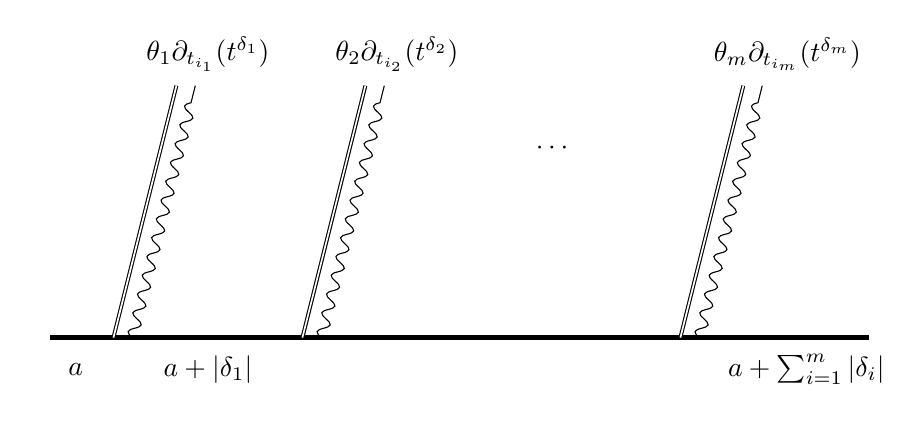
\begin{tikzpicture}[scale=0.8,auto]
\draw[line width=2pt] (-8,0) -- (5,0);
\draw[snake=coil,segment aspect=0, segment amplitude=2pt, segment length=7pt] (-6.7,0) -- (-5.7,4);
\draw[double] (-7,0) -- (-6,4);
\node (1t) at (-5.5,4.5) {$\theta_1 \partial_{t_{i_1}}(t^{\delta_1})$};
\draw[snake=coil,segment aspect=0, segment amplitude=2pt, segment length=7pt] (-3.7,0) -- (-2.7,4);
\draw[double] (-4,0) -- (-3,4);
\node (2t) at (-2.5,4.5) {$\theta_2 \partial_{t_{i_2}}(t^{\delta_2})$};
\node (dots) at (0,3) {$\cdots$};
\draw[snake=coil,segment aspect=0, segment amplitude=2pt, segment length=7pt] (2.3,0) -- (3.3,4);
\draw[double] (2,0) -- (3,4);
\node (nt) at (3.7,4.5) {$\theta_m \partial_{t_{i_m}}(t^{\delta_m})$};
\node (1) at (-7.6,-0.5) {$a$};
\node (2) at (-5.5,-0.5) {$a + |\delta_1|$};
\node (m) at (4,-0.5) {$a + \sum_{i=1}^m |\delta_i|$};
\end{tikzpicture}
\centering
\caption{Depiction of a process contributing soft factors. The thick line represents a state containing $a$ $\theta$'s and $t$'s, and the labels indicate the virtual weight fo the state obtained by cutting the diagram vertically at the given time.}\label{fig:tapesofU}
\end{figure}

There is also a $\zeta$ which appears as $\zeta \nabla$ in $\phi_\infty$, which contributes a scalar factor immediately after every B-type vertex. To be precise, $(\zeta \vAt_{\AA})^m \zeta$ will contribute
\be\label{eq:diagram_for_zeta_eq_b}
\frac{1}{a} \frac{1}{a + |\delta_1|} \frac{1}{a + |\delta_1| + |\delta_3|} \cdots \frac{1}{a + |\delta_1| + \cdots + |\delta_m|}\,.
\ee

\subsection{Diagrams for composition}\label{section:feynman_diagram_3}

The final piece to understanding Feynman diagrams is to have a diagrammatic representation of the composition operator
\[
\mu_2: \HH(Y, Z) \otimes \HH(X, Y) \lto \HH(X,Z)
\]
once we have expressed all the involved mapping spaces, such as $\Hom_k(\widetilde{X}, \widetilde{Y})$, in terms of creation and annihilation operators. In addition to the spaces $\widetilde{X} = \bigwedge F_\xi$ and $\widetilde{Y} = \bigwedge F_\eta$ underlying the matrix factorisations $X,Y$ we now introduce odd generators $\varepsilon_1,\ldots,\varepsilon_t$ and $F_\varepsilon = \bigoplus_{i=1}^t k \varepsilon_i$ and $\nZ_2$-graded $k$-module
\be
\widetilde{Z} = \bigwedge F_\varepsilon = \bigwedge\big( k \varepsilon_1 \oplus \cdots \oplus k \varepsilon_t \big)\,.
\ee
underlying a Koszul matrix factorisation $Z = \widetilde{X} \otimes R$. 

Note that for $\omega, \omega' \in \bigwedge F_\theta$ and $\alpha \in \Hom_k(\widetilde{Y}, \widetilde{X}), \beta \in \Hom_k(\widetilde{Z}, \widetilde{Y})$
\begin{gather*}
\mu_2\Big( [ \omega \otimes z_i \otimes \alpha ] \otimes [ \omega' \otimes z_j \otimes \beta ] \Big) \\
= (-1)^{|\alpha||\omega'|} \sum_{k=1}^\mu \sum_{\delta} \Gamma^{ij}_{k \delta} \cdot \omega \wedge \omega' \otimes z_k \otimes \alpha \beta \otimes t^{\delta}\,.
\end{gather*}


Recall $\nu$ from Lemma \ref{lemma:iso_nu} and the ``bar convention'' of Definition \ref{defn:bar_convention}.

\begin{lemma}\label{lemma:mixedr2_0} The diagram
\be
\xymatrix@C+2pc@R+2pc{
\Hom_k( \widetilde{Y}, \widetilde{Z} ) \otimes \Hom_k( \widetilde{X}, \widetilde{Y} ) \ar[d]_-{\nu \otimes \nu} \ar[r]^-{- \circ -} & \Hom_k( \widetilde{X}, \widetilde{Z} ) \ar[d]^-\nu\\
\big( \bigwedge F_\varepsilon \otimes \bigwedge F_{\Bar{\eta}} \big) \otimes \big( \bigwedge F_\eta \otimes \bigwedge F_{\Bar{\xi}} \big) \ar[d]_-{\exp( \sum_i \Bar{\eta}_i^* \eta_i^* )} & \bigwedge F_\varepsilon \otimes \bigwedge F_{\Bar{\xi}} \ar@{=}[d]\\
\big( \bigwedge F_\varepsilon \otimes \bigwedge F_{\Bar{\eta}} \big) \otimes \big( \bigwedge F_\eta \otimes \bigwedge F_{\Bar{\xi}} \big) \ar[r]_-P & \bigwedge F_\varepsilon \otimes \bigwedge F_{\Bar{\xi}}
}
\ee
commutes, where $P$ denotes the projection onto the subspace with no $\Bar{\eta}$'s or $\eta$'s.
\end{lemma}

\begin{lemma}\label{lemma:mixedr2_1} The diagram
\be
\xymatrix@C+2pc@R+2pc{
\Hom_k( \widetilde{X}, \widetilde{Y} ) \otimes \Hom_k( \widetilde{X}, \widetilde{X} ) \ar[d]_-{\nu \otimes \rho^{-1}} \ar[r]^-{- \circ -} & \Hom_k( \widetilde{X}, \widetilde{Y} ) \ar[d]^-\nu\\
\big( \bigwedge F_\eta \otimes \bigwedge F_{\Bar{\xi}} \big) \otimes \big( \bigwedge F_\xi \otimes \bigwedge F_{\Bar{\xi}} \big) \ar[d]_-{\exp( -\sum_i \Bar{\xi}_i^* \xi_i^* )} & \bigwedge F_\eta \otimes \bigwedge F_{\Bar{\xi}} \\
\big( \bigwedge F_\eta \otimes \bigwedge F_{\Bar{\xi}} \big) \otimes \big( \bigwedge F_\xi \otimes \bigwedge F_{\Bar{\xi}} \big) \ar[r]_-P & \bigwedge F_\eta \otimes \bigwedge F_{\Bar{\xi}} \otimes \bigwedge F_{\Bar{\xi}} \ar[u]_-{1 \otimes m}
}
\ee
commutes, where $P$ projects out the $F_{\xi}$ and $m$ is multiplication in the exterior algebra.
\end{lemma}

The upshot is that we can think of a composition operator $\mu_2$ at a vertex in our trees as the combination of a boundary condition $P$ together with new types of interaction vertices. In the case of Lemma \ref{lemma:mixedr2_0} we call this a (D.1) interaction, in which $\Bar{\eta}^* \eta_i^*$ which couples an incoming $\eta_i$ in the right branch with an incoming $\Bar{\eta}_i$ (which we view as an $\eta_i$ travelling upward) in the left branch. More directly: an incoming $\eta_i$ on the right hand branch can (and indeed \emph{must} in light of $P$) bend around and travel up the left hand branch, as in Figure \ref{fig:run_around_corners}. Similarly we denote by (D.2) the interactions arising from Lemma \ref{lemma:mixedr2_1}.

\begin{figure}
\begin{center}
\begin{tabular}{ >{\centering}m{8cm} >{\centering}m{6cm} }
\textbf{(D.1) $+1$}
\vspace{0.1cm}
\[
\xymatrix@C+2pc@R+3pc{
& & \ar[dl]^-{\eta_i} \\
& \bullet \ar[ul]^-{\eta_i}
}
\]
&
\textbf{(D.2) $-1$}
\vspace{0.1cm}
\[
\xymatrix@C+2pc@R+3pc{
& & \ar[dl]^-{\xi_i} \\
& \bullet \ar[ul]^-{\xi_i}
}
\]
\end{tabular}
\end{center}
\centering
\caption{The interactions (D.1),(D.2).}\label{fig:run_around_corners}
\end{figure}

\begin{lemma}\label{lemma:mixedr2_2} The diagram
\be
\xymatrix@C+2pc@R+2pc{
\Hom_k( \widetilde{Y}, \widetilde{Y} ) \otimes \Hom_k( \widetilde{X}, \widetilde{Y} ) \ar[d]_-{\rho^{-1} \otimes \nu} \ar[r]^-{- \circ -} & \Hom_k( \widetilde{X}, \widetilde{Y} ) \ar[d]^-\nu\\
\big( \bigwedge F_\eta \otimes \bigwedge F_{\Bar{\eta}} \big) \otimes \big( \bigwedge F_\eta \otimes \bigwedge F_{\Bar{\xi}} \big) \ar[d]_-{\exp( -\sum_i \Bar{\eta}_i^* \eta_i^* )} & \bigwedge F_\eta \otimes \bigwedge F_{\Bar{\xi}} \\
\big( \bigwedge F_\eta \otimes \bigwedge F_{\Bar{\eta}} \big) \otimes \big( \bigwedge F_\eta \otimes \bigwedge F_{\Bar{\xi}} \big) \ar[r]_-P & \bigwedge F_\eta \otimes \bigwedge F_\eta \otimes \bigwedge F_{\Bar{\xi}} \ar[u]_-{m \otimes 1}
}
\ee
commutes, where $P$ projects out the $\bigwedge F_{\Bar{\eta}}$ and $m$ is multiplication in the exterior algebra. The operator $\eta_i^*$ in the exponential acts on the third tensor factor.
\end{lemma}

The lemma says that at an internal vertex of the tree, where interactions on the left hand branch are presented using $\rho$ and on the right hand branch using $\nu$, the boundary condition imposed by $P$ is that there are no upward travelling $\eta$'s entering the vertex from below, while the interaction vertices allow downward travelling $\eta$'s on the right branch to convert to upward travelling $\eta$'s on the left (one can also read this as ``the only possible origin of an upward travelling $\eta$ on the left branch is a downward travelling $\eta$ on the right branch''). We denote this interaction vertex also by (D.2).

The last remark that needs to be made is that, in box of the mixed cases there are still multiplications in the final presentation. For example there is a $1 \otimes m$ in Lemma \ref{lemma:mixedr2_1}. The reason for this is that upward travelling $\xi$'s entering the vertex can either continue upwards into the left branch, or into the right branch. Diagrammatically, what this means is that an annihilation operator $\Bar{\xi}_i^*$, when we try to commute it from left to right in an operator expression, encounters such a vertex and generates two terms (since it is a graded derivation)
\be\label{eq:xi_is_derivation}
\Bar{\xi}_i^* m = m (\Bar{\xi}_i^* \otimes 1) + m( 1 \otimes \Bar{\xi}_i^* )
\ee
which correspond respectively to the $\xi_i$ travelling up the left branch or the right. A similar description applies to the $m \otimes 1$ in Lemma \ref{lemma:mixedr2_2}. 

\begin{remark} What about $z_i$ meet $z_j$ vertices using $\Gamma$? These are part of $\mu_2$.
\end{remark}

\subsection{Putting it all together}\label{section:feynman_diagram_4}

We now return to the broader picture, and integrate the previous sections into a complete method for reasoning about higher operations $\rho_k$ using Feynman diagrams. Such operations are parametrised by matrix factorisations $X_0,\ldots,X_k \in \AA$ which we assume to be Koszul, with underlying graded $k$-module $\widetilde{X}_i = \bigwedge F^{(i)}_\xi$. Once we choose for each pair $(i,i+1)$ and $(0,n)$ either $\nu$ or $\rho$ to present the mapping spaces $\BB(X_i, X_{i+1})$ as a tensor product of exterior algebras, $\rho_k$ is a $k$-linear map
\be
\rho_k: \bigotimes_{i=0}^{k-1}\Big[ R/I \otimes \bigwedge F_{\xi}^{(i+1)} \otimes \bigwedge F_{\Bar{\xi}}^{(i)} \Big][1] \lto \Big[ R/I \otimes \bigwedge F_{\xi}^{(n)} \otimes \bigwedge F_{\Bar{\xi}}^{(0)} \Big] [1]\,.
\ee
We explain how to evaluate this linear map on an input tensor using Feynman diagrams. The operator $\rho_k$ is defined by \eqref{eq:rho_kintermsoftrees} to be a sum of operators $\rho_T$ indexed by $T \in \cat{BT}_k$. The description of such an operator in terms of Feynman diagrams is reached in several stages, which are summarised by the Feynman rules in Definition \ref{defn:feynman_rules} below.
\\

\textbf{Stage one: expansion.} The operator $\rho_T$ is defined as a composition of operators
\be
\sigma_\infty, \phi_\infty, e^{\delta}, e^{-\delta}, r_2, \pi\,.
\ee
These in turn may be written, with some signs and factorials, in terms of the operators\footnote{For the reader's convenience, here is a cheatsheet: for $\zeta$ see Section \ref{section:propagator}, $\vAt$ is the Atiyah class of Definition \ref{defn:atiyah_class}, $\nabla$ the chosen connection from Corollary \ref{corollary:nabla_sigma}, $\sigma$ the chosen section of the quotient map $\pi: R \lto R/I$, for $\delta$ see Definition \ref{defn:important_operators}, $r_2$ is the forward suspended multiplication in $\AA'_\theta$.}
\be\label{eq:goodlist_2}
\zeta, \vAt, \nabla, \sigma, \delta, r_2, \pi\,.
\ee
With a fixed input to $\rho_T$ we may use Lemma \ref{prop:replacer2} to pull out a global sign, replace $r_2$ by $\mu_2$ and evaluate the tree without further Koszul signs (note that we are now evaluating operators inserted on the mirrored tree). The signs and factorials involved are accounted for carefully in Definition \ref{defn:feynman_rules} below; for clarity we omit them in the present discussion.

At this point, we have to evaluate compositions of the operators in the list \eqref{eq:goodlist_2} counted with signs and factorials from the exponentials, similar to \eqref{eq:contrib_feynman}. We choose the $\nu$ or $\rho$ presentation for each edge of the tree and expand occurrences of $\vAt, \nabla, \delta$ using \eqref{eq:a1vertex}-\eqref{eq:a4vertex}, \eqref{eq:c1vertex},\eqref{eq:c2vertex} in the $\nu$ cases and \eqref{eq:a3vertex_rho},\eqref{eq:a4vertex_rho},\eqref{eq:c1vertex_rho},\eqref{eq:c2vertex_rho} in the $\rho$ cases. We replace the occurrences of $\mu_2$ using the lemmas of Section \ref{section:fenyman_diagram_2} with additional exponentials and occurrences of $m$. As a result, we now have a sum of trees with operators from
\be\label{eq:goodlist_3}
\zeta, \theta, \theta^*, z, z^*, t, \partial_t, \xi, \xi^*, \Bar{\xi}, \Bar{\xi}^*, m, \pi
\ee
In this expression the remaining terms that are \emph{not} creation and annihilation operators are occurrences of $\zeta$ and the multiplications $m$ on exterior algebras from Lemma \ref{lemma:mixedr2_1} and Lemma \ref{lemma:mixedr2_2}. At this point all the relevant virtual degrees are fixed, and we can calculate the scalar contribution from the $\zeta$ operators. This completes the expansion stage.
\\

\textbf{Stage two: reduction to normal form.} A contraction of monomials in creation and annihilation operators is said to be in \emph{normal form} if every annihilation operator is to the right of every creation operator (TODO). After stage one, the summands contributing to $\rho_T$ are \emph{not} in normal form, but there is a rewrite process that converts any summand into a sum of operators in normal form. The sums arise because the rewrite process is ``nondeterministic'' in the sense that various stages there are choices, and each choice generates two separate diagrams. A Feynman diagram is \emph{precisely a record of a series of such choices made during the rewrite process.} Taking each annihilation operators in turn, we use the available (anti)commutation relations to move it to the right. Take the leftmost fermionic annihilation operator $\omega^*$ in a given operator (that is, the lowest operator in the tree) and start to commute it to the right (that is, up the tree). The only things that can happen are
\begin{itemize}
\item $\omega^*$ meets an $m$ (see \eqref{eq:xi_is_derivation}) and generates two additional terms (TODO: diagram)
\item $\omega^*$ meets an $\omega$ and generates two additional terms
\[
\omega^* \omega = - \omega \omega^* + 1
\]
TODO: diagrams.
\item $\omega^*$ meets the vacuum at the top of the tree and becomes zero.
\end{itemize}
In the first case the line entering the interaction vertex corresponding to $\omega^*$ follows either the left or right branch (depending on which summand we chose), in the second case the line either passes through the vertex, or is connected to the outgoing $\omega$ at that vertex (depending on which summand we chose) and in the third case the summand is zero and needs no diagram. 

Now on our tree we draw all the occurring interaction vertices. Next we have to figure out how to ``hook up'' the lines emanating from each of these vertices. There are many choices, each of which gives their own Feynman diagram.

%\begin{example} Give a picture of two interaction vertices being joined by a $\theta$, or some such, to give a local instance of how this works.
%\end{example}

We now perform the same process for the new leftmost fermionic annihilation operator, and so on, until we have only operators from the list
\be\label{eq:goodlist_3}
z, z^*, t, \partial_t, \xi, \Bar{\xi}, m, \pi
\ee
Note that any diagram which still contains a fermionic creation operator $\theta$ at this point must contribute zero, since we apply $\pi$ at the bottom of our trees (so no diagram with an outgoing $\theta$ or $t^\delta$ can contribute). Next we connect up all the $z,z^*$ lines, and begin to commute the leftmost bosonic annihilation operator $\partial_t$ to the right, hooking up boson lines according to the same principles as above. Once this is done, we are left with operators
\be\label{eq:goodlist_3}
z, \xi, \Bar{\xi}, m, \pi
\ee
evaluating which gives a wedge product of terms in $R/I \otimes \bigwedge F_\xi^{(n)} \otimes \bigwedge F_{\Bar{\xi}}^{(0)}$, and this is the output of this particular summand of $\rho_T$, which is to be counted with the various coefficients and signs collected during the above process.

%\begin{remark} The non-Koszul case is treated in the same way, we just treat the tensor factor $\Hom_k(\widetilde{X}, \widetilde{Y})$ like $R/I$.
%\end{remark}

Summarising the above, here are the final Feynman rules for evaluating $\rho_{T'}$, which involves Feynman diagrams on the mirrored tree $T$ according to Lemma \ref{??}. Suppose $T$ has $k$ leaves and that we wish to compute the coefficient $C_\tau \in k$ of $\tau$ in $\rho_{T'}( \xi_k, \ldots, \xi_1 )$. Choose a presentation $\nu$ or $\rho$ for each edge in the tree.

NOTE: we use language like "higher up the tree" and for m's we need it to, we need to properly define this.

\begin{definition}[(Feynman rules)]\label{defn:feynman_rules} The coefficient $C_\tau$ is a sum $\sum_{F \in \cat{F}} C_{\tau, F}$ of coefficients $C_{\tau, F}$ associated to Feynman diagrams $F$. To enumerate the possible Feynman diagrams, first draw $\xi_1,\ldots,\xi_k$ and $\tau$ as collections of incoming and outgoing particle lines on the tree $T$, respectively, and then choose for each
\begin{itemize}
\item \textbf{input} a finite number of A-type vertices, followed immediately below in the tree by a finite number of C-type vertices,
\item \textbf{internal vertex} a finite number of vertices of type D,
\item \textbf{internal edge} a finite number of C-type vertices, followed by a B-type vertex, followed by a finite number of A-type vertices, followed by C-type vertices
\item and for the \textbf{outgoing edge} a finite number of C-type vertices.
\end{itemize}
Draw the chosen interaction vertices, and then choose a way of connecting incoming lines at vertices lower down the tree, to outgoing lines of the same type higher up the tree.\footnote{Since the only lines incident with the incoming and outgoing boundary of the tree are those arising from the $\xi_i$ and $\tau$, in particular no ``virtual particles'' ($t$'s or $\theta$'s) may enter or leave the diagram.} In each case the number of A, C, D-type vertices chosen may be zero, but every internal edge has precisely one B-type vertex. These choices parametrise a finite set of Feynman diagrams $\cat{F}$. The coefficient $C_{\tau, F}$ contributed by a particular diagram is the product of
\begin{itemize}
\item The coefficients associated to each interaction vertex as given above (this includes the scalar factor from the $\partial_{t_k}(t^\delta)$ in A-type vertices).
\item For each collection of $n$ C-type vertices a factorial $\frac{1}{n!}$ and if the collection immediately preceedes a B-type vertex or the exist node, a sign $(-1)^n$ (from $e^{-\delta}$ versus $e^\delta$).
\item A factor of $-1$ for every time two fermion lines cross in the diagram.
\item $\zeta$ factors (see Section \ref{section:fenyman_diagram_2}).
\item For each A-type vertex there is a sign factor $-1$ (from the $(-1)^m$ factors in $\sigma_\infty,\phi_\infty$).
\item For each (D.2)-type vertex there is a sign factor $-1$ (see Section \ref{section:feynman_diagram_3}).
\item The sign from Lemma \ref{prop:replacer2}.
\end{itemize}
\end{definition}

\begin{remark}\label{remark:boson_symmetry} Recall that we draw an interaction vertex $v$ with an outgoing line labelled $t^\delta = t_1^{\delta_1} \cdots t_n^{\delta_n}$ in our pictures, the convention is that such a line stands for $|\delta|$ separate lines labelled $t_i$ for some $i$. The above description of the Feynman rules involves choosing, for each such $v$, a series of B-type vertices to pair with each of these lines. 

This leads to $\delta_1! \cdots \delta_n!$ otherwise identical diagrams, in which the only difference is \emph{which} of the $\delta_i$ lines labelled $t_i$ is paired with which $(B)_i$ vertex. The usual convention is to draw just one such diagram, counted with a symmetry factor $\delta_1! \cdots \delta_n!$.
\end{remark}

\begin{example} We now explicate the above process in the example of $W = \frac{1}{5} x^5$ and matrix factorisations $X,Y$ in the above notation (generated by $\xi$ and $\eta$)
\begin{align}
X &= \big( \bigwedge(k \xi) \otimes k[x], x^2 \xi^* + \frac{1}{5} x^3 \xi \big)\\
Y &= \big( \bigwedge(k \eta) \otimes k[x], x^3 \eta^* + \frac{1}{5} x^2 \eta \big)
\end{align}
so $f = x^2, u = x^3, g = \frac{1}{5}x^3, v = \frac{1}{5} x^2$. We aim to calculate
\[
\rho_3: \HH_{\BB}(Y,Y) \otimes \HH_{\BB}(X, Y) \otimes \HH_{\BB}(X,X) \lto \HH_{\BB}(X,Y)
\]
on an example input. We set $t = \partial_x W = x^4$ and choose our connection $\nabla$ and operators $\partial_t$ as in Example \ref{example:dt_xd} with $d = 4$. For the homotopies $\lambda^Y, \lambda^X$ we use the default choices of Remark \ref{remark:default_homotopies}, so that
\begin{align*}
\lambda^X &= \partial_x( d_X ) = 2 x \xi^* + \frac{3}{5} x^2 \xi && F^X = 2x, \quad G^X = \frac{3}{5} x^2\\
\lambda^Y &= \partial_x( d_Y ) = 3 x \eta^* + \frac{2}{5} x \eta && F^Y = 3x, \quad G^Y = \frac{2}{5} x
\end{align*}
To compute the coefficients associated to all the interaction vertices, we need to compute for various $r \in R$ the coefficients $r_{(m,\alpha)}$ (see Definition \ref{defn:rsharp}) as well as the tensor $\Gamma$. This involves fixing the $k$-basis $R/I = k[x]/x^4 = k1 \oplus kx \oplus kx^2 \oplus kx^3$ that is, $z_h = x^h$ for $0 \le h \le 3$, and the section $\sigma(x^i) = x^i$. Then for example
\[
x^3 = 1 \cdot \sigma( x^3 ) t^0
\]
and in general $(x^a)_{(m,\alpha)} = \delta_{m = a} \delta_{\alpha = 0}$ for $0 \le a \le 3$. Since all the polynomials occurring in $f,g,u,v,F,G$ have degree $\le 3$ these coefficients are all easily calculated as delta functions in this way. The tensor $\Gamma$ encodes the multiplication in $R/I$ and is given by Definition \ref{defn_gamma} for $0 \le m,h \le 3$ by
\[
\Gamma^{mh}_{l \beta} = \delta_{m+h \le 3}\delta_{l = m+h}\delta_{\beta = 0} + \delta_{m+h > 3} \delta_{l = m+h-4} \delta_{\beta = 1}\,.
\]
To present interaction vertices as creation and annihilation operators we use $\rho$ on all edges of the tree involving pairs $(Y,Y)$ and $(X,X)$ and $\nu$ on edges involving $(X,Y)$. Such edges involve $\eta$'s travelling downward and $\xi$'s travelling upward, and the interactions are (recall our convention is to write $h$ for $z_h$ in these diagrams):
\begin{center}
\begin{tabular}{ >{\centering}m{5cm} >{\centering}m{5cm} >{\centering}m{5cm} }
\textbf{(A.1)${}^\nu_{h > 0}$ $+1$}
\vspace{0.1cm}
\[
\xymatrix@C+1pc@R+1.5pc{
& \ar@{.}[d]^-{h} & \ar[dl]^-{\eta}\\
& \bullet \ar@{=}[dl]^-{\theta} \ar@{.}[d]^-{h-1}\\
& &
}
\] %$\theta z_{h-1} z_h^* \eta^*$
&
\textbf{(A.2)${}^\nu_{h > 1}$ $+\frac{1}{5}$}
\vspace{0.1cm}
\[
\xymatrix@C+1pc@R+1.5pc{
& \ar@{.}[d]^-{h}\\
& \bullet \ar@{=}[dl]_-{\theta} \ar@{.}[d]^-{h-2} \ar[dr]^-{\eta}\\
& &
}
\]
%$\theta z_{h-2} \eta z_h^*$
&
\textbf{(A.3)${}^\nu_{h>1}$ $-1$}
\vspace{0.1cm}
\[
\xymatrix@C+1pc@R+1.5pc{
& \ar@{.}[d]^-{h}\\
& \bullet \ar@{=}[dl]_-{\theta} \ar@{.}[d]^-{h-2} \\
& & \ar[ul]_-{\xi}
}
\]
%$\theta z_{h-2} \xi^* z_h^*$
\end{tabular}
\end{center}

\begin{center}
\begin{tabular}{ >{\centering}m{5cm} >{\centering}m{5cm} >{\centering}m{5cm} }
\textbf{(A.4)${}^\nu_{h>0}$ $+\frac{1}{5}$}
\vspace{0.1cm}
\[
\xymatrix@C+1pc@R+1.5pc{
& \ar@{.}[d]^-{h} &\\
& \bullet \ar[ur]_-{\xi} \ar@{=}[dl]^-{\theta} \ar@{.}[d]^-{h-1} \\
& &
}
\] %$\theta z_{h-1} z_h^*(\xi^*)^*$
&
\textbf{(B)}
\vspace{0.1cm}
\[
\xymatrix@R+1.5pc{
\ar@{~}[d]^-{t}\\
\bullet \ar@{=}[d]^-{\theta}\\
\;
}
\]
& 
\textbf{(C.1)${}^\nu_{h\le2}$ $3$}
\vspace{0.1cm}
\[
\xymatrix@C+1pc@R+1.5pc{
\ar[dr]_-{\eta} & \ar@{.}[d]^-{h} & \ar@{=}[dl]^-{\theta}\\
& \bullet \ar@{.}[d]^-{h+1} \\
& &
}
\] %$z_{h+1} \eta^* z_h^* \theta^*$
\end{tabular}
\end{center}

\begin{center}
\begin{tabular}{ >{\centering}m{5cm} >{\centering}m{5cm} >{\centering}m{5cm} }
\textbf{(C.1)${}^\nu_{h>2}$ $3$}
\vspace{0.1cm}
\[
\xymatrix@C+1pc@R+1.5pc{
\ar[dr]_-{\eta} & \ar@{.}[d]^-{h} & \ar@{=}[dl]^-{\theta}\\
& \bullet \ar@{.}[d]^-{h-3} \ar@{~}[dl]^-{t}\\
& &
}
\] %$z_{h-3} t \eta^* z_h^* \theta^*$
&
\textbf{(C.2)$^\nu_{h \le 2}$ $+\frac{2}{5}$}
\vspace{0.1cm}
\[
\xymatrix@C+1pc@R+1.5pc{
& \ar@{.}[d]^-{h} & \ar@{=}[dl]^-{\theta} \\
& \bullet \ar[dl]^-{\eta}\ar@{.}[d]^-{h+1} \\
& &
}
\]%$z_{h+1} \eta z_h^* \theta^*$
&
\textbf{(C.2)$^\nu_{h > 2}$ $+\frac{2}{5}$}
\vspace{0.1cm}
\[
\xymatrix@C+1pc@R+1.5pc{
& \ar@{.}[d]^-{h} & \ar@{=}[dl]^-{\theta} \\
& \bullet \ar[dl]^-{\eta}\ar@{.}[d]^-{h-3} \ar@{~}[dr]^-{t}\\
& &
}
\] %$z_{h-3} t \eta z_h^* \theta^*$
\end{tabular}
\end{center}

On the edges involving $X$ purely, where we are using the $\rho$ presentation, we have the following interaction vertices (we omit the B-type which is as above):\footnote{Insanity: the $(A.3)_{h>1}^\rho$ interaction has different signs according to $\nu$ and $\rho$.}

\begin{center}
\begin{tabular}{ >{\centering}m{5cm} >{\centering}m{5cm} >{\centering}m{5cm} }
\textbf{(A.1)${}^{X,\rho}_{h>1}$ $+1$}
\vspace{0.1cm}
\[
\xymatrix@C+1pc@R+1.5pc{
& \ar@{.}[d]^-{h} & \ar[dl]^-{\xi}\\
& \bullet \ar@{=}[dl]_-{\theta} \ar@{.}[d]^-{h-2} \\
& & &
}
\] %$\theta z_{h-2} (\xi^* \otimes 1) z_h^*$
&
\textbf{(A.4)${}^{X,\rho}_{h>0}$ $\frac{1}{5}$}
\vspace{0.1cm}
\[
\xymatrix@C+1pc@R+1.5pc{
& \ar@{.}[d]^-{h} &\\
& \bullet \ar[ur]_-{\xi} \ar@{=}[dl]^-{\theta} \ar@{.}[d]^-{h-1}\\
& &
}
\] %$\theta z_{h-1} z_h^*(1 \otimes (\xi^*)^*)$
&
\textbf{(C.1)${}^{X,\rho}_{h \le 2}$ $2$}
\vspace{0.1cm}
%$z_{l} t^\delta \xi_i^* z_h^* \theta_k^*$
\[
\xymatrix@C+1pc@R+1.5pc{
\ar[dr]_-{\xi} & \ar@{.}[d]^-{h} & \ar@{=}[dl]^-{\theta}\\
& \bullet \ar@{.}[d]^-{h+1}\\
& &
}
\]
\end{tabular}
\end{center}

\begin{center}
\begin{tabular}{ >{\centering}m{5cm} >{\centering}m{5cm} >{\centering}m{5cm} }
\textbf{(C.1)${}^{X,\rho}_{h > 2}$ $2$}
\vspace{0.1cm}
%$z_{l} t^\delta \xi_i^* z_h^* \theta_k^*$
\[
\xymatrix@C+1pc@R+1.5pc{
\ar[dr]_-{\xi} & \ar@{.}[d]^-{h} & \ar@{=}[dl]^-{\theta}\\
& \bullet \ar@{.}[d]^-{h-3} \ar@{~}[dl]^-{t}\\
& &
}
\]
&
\textbf{(C.2)${}^{X,\rho}_{h \le 1}$ $\frac{3}{5}$}
\vspace{0.1cm}
%$z_{l} t^\delta \xi z_h^* \theta^*$
\[
\xymatrix@C+1pc@R+1.5pc{
& \ar@{.}[d]^-{h} & \ar@{=}[dl]^-{\theta} \\
& \bullet \ar[dl]^-{\xi}\ar@{.}[d]^-{h+2}\\
& &
}
\]
&
\textbf{(C.2)${}^{X,\rho}_{h > 1}$ $\frac{3}{5}$}
\vspace{0.1cm}
%$z_{l} t^\delta \xi z_h^* \theta^*$
\[
\xymatrix@C+1pc@R+1.5pc{
& \ar@{.}[d]^-{h} & \ar@{=}[dl]^-{\theta} \\
& \bullet \ar[dl]^-{\xi}\ar@{.}[d]^-{h-2} \ar@{~}[dr]^-{t}\\
& &
}
\]
\end{tabular}
\end{center}

\begin{center}
\begin{tabular}{ >{\centering}m{6cm} >{\centering}m{6cm} }
\textbf{(C.3)${}^{X,\rho}_{h \le 2}$ $2$}
\vspace{0.1cm}
% $z_{l} t^\delta \Bar{\xi}_i z_h^* \theta_k^*$
\[
\xymatrix@C+2pc@R+1.5pc{
& \ar@{.}[d]^-{h} & \ar@{=}[dl]^-{\theta} \\
& \bullet \ar@{.}[d]^-{h+1} \\
\ar[ur]^-{\xi} & &
}
\]
&
\textbf{(C.3)${}^{X,\rho}_{h > 2}$ $2$}
\vspace{0.1cm}
% $z_{l} t^\delta \Bar{\xi}_i z_h^* \theta_k^*$
\[
\xymatrix@C+2pc@R+1.5pc{
& \ar@{.}[d]^-{h} & \ar@{=}[dl]^-{\theta} \\
& \bullet \ar@{.}[d]^-{h-3} \ar@{~}[dr]^-{t}\\
\ar[ur]^-{\xi} & &
}
\]
\end{tabular}
\end{center}

On edges involving $Y$ purely, where again we use the $\rho$ presentation, we have:

\begin{center}
\begin{tabular}{ >{\centering}m{5cm} >{\centering}m{5cm} >{\centering}m{5cm} }
\textbf{(A.1)${}^{Y,\rho}_{h > 0}$ $1$}
\vspace{0.1cm}
%$\theta z_{h-1} (\eta^* \otimes 1) z_h^*$
\[
\xymatrix@C+1pc@R+1.5pc{
& \ar@{.}[d]^-{h} & \ar[dl]^-{\eta}\\
& \bullet \ar@{=}[dl]_-{\theta} \ar@{.}[d]^-{h-1} \\
& &
}
\]
&
\textbf{(A.4)${}^{Y,\rho}_{h>1}$ $\frac{1}{5}$}
\vspace{0.1cm}
%$\theta_k z_{h-2} z_h^*(1 \otimes (\eta^*)^*)$
\[
\xymatrix@C+1pc@R+1.5pc{
& \ar@{.}[d]^-{h} &\\
& \bullet \ar[ur]_-{\eta} \ar@{=}[dl]^-{\theta} \ar@{.}[d]^-{h-2} \\
& &
}
\]
&
\textbf{(C.1)${}^{Y,\rho}_{h \le 2}$ $3$}
\vspace{0.1cm}
%$z_{l} t^\delta \eta^* z_h^* \theta^*$
\[
\xymatrix@C+1pc@R+1.5pc{
\ar[dr]_-{\eta} & \ar@{.}[d]^-{h} & \ar@{=}[dl]^-{\theta}\\
& \bullet \ar@{.}[d]^-{h+1} \\
& &
}
\]
\end{tabular}
\end{center}

\begin{center}
\begin{tabular}{ >{\centering}m{5cm} >{\centering}m{5cm} >{\centering}m{5cm} }
\textbf{(C.1)${}^{Y,\rho}_{h>2}$ $3$}
\vspace{0.1cm}
%$z_{l} t^\delta \eta^* z_h^* \theta^*$
\[
\xymatrix@C+1pc@R+1.5pc{
\ar[dr]_-{\eta} & \ar@{.}[d]^-{h} & \ar@{=}[dl]^-{\theta}\\
& \bullet \ar@{.}[d]^-{h-3} \ar@{~}[dl]^-{t}\\
& &
}
\]
&
\textbf{(C.2)${}^{Y,\rho}_{h \le 2}$ $\frac{2}{5}$}
\vspace{0.1cm}
%$z_{l} t^\delta \xi_i z_h^* \theta_k^*$
\[
\xymatrix@C+2pc@R+1.5pc{
& \ar@{.}[d]^-{h} & \ar@{=}[dl]^-{\theta} \\
& \bullet \ar[dl]^-{\eta}\ar@{.}[d]^-{h+1}\\
& &
}
\]
&
\textbf{(C.2)${}^{Y,\rho}_{h > 2}$ $\frac{2}{5}$}
\vspace{0.1cm}
%$z_{l} t^\delta \xi_i z_h^* \theta_k^*$
\[
\xymatrix@C+2pc@R+1.5pc{
& \ar@{.}[d]^-{h} & \ar@{=}[dl]^-{\theta} \\
& \bullet \ar[dl]^-{\eta}\ar@{.}[d]^-{h-3} \ar@{~}[dr]^-{t}\\
& &
}
\]
\end{tabular}
\end{center}

\begin{center}
\begin{tabular}{ >{\centering}m{6cm} >{\centering}m{6cm} }
\textbf{(C.3)${}^{Y,\rho}_{h \le 2}$ $3$}
\vspace{0.1cm}
%$z_{l} t^\delta \Bar{\xi}_i z_h^* \theta_k^*$
\[
\xymatrix@C+2pc@R+1.5pc{
& \ar@{.}[d]^-{h} & \ar@{=}[dl]^-{\theta} \\
& \bullet \ar@{.}[d]^-{h+1}\\
\ar[ur]^-{\eta} & &
}
\]
&
\textbf{(C.3)${}^{Y,\rho}_{h > 2}$ $3$}
\vspace{0.1cm}
%$z_{l} t^\delta \Bar{\xi}_i z_h^* \theta_k^*$
\[
\xymatrix@C+2pc@R+1.5pc{
& \ar@{.}[d]^-{h} & \ar@{=}[dl]^-{\theta} \\
& \bullet \ar@{.}[d]^-{h-3} \ar@{~}[dr]^-{t}\\
\ar[ur]^-{\eta} & &
}
\]
\end{tabular}
\end{center}

Suppose we want to evaluate the forward suspended product
\[
\rho_3: \HH_{\BB}(X,X)[1] \otimes \HH_{\BB}(X,Y)[1] \otimes \HH_{\BB}(Y,Y)[1] \lto \HH_{\BB}(X,Y)[1]
\]
on an input tensor
\[
x^2 \xi \otimes x \eta \Bar{\xi} \otimes x^3 \Bar{\eta} = z_2 \xi \otimes z_1 \eta \Bar{\xi} \otimes z_3 \Bar{\eta}\,.
\]
There are contributions to the output from each of the two trees with three leaves, and we examine one Feynman diagram contributed by our standard tree $T$ of Figure \ref{eq:explicit_tree_operator}. We are in the situation examined in the proof of Lemma \ref{prop:replacer2}, with
\[
\rho_T( z_2 \xi, z_1 \eta \Bar{\xi}, z_3 \Bar{\eta} ) = \pi e^{-\delta} \mu_2\Big\{ e^{\delta} \phi_\infty e^{-\delta} \mu_2\Big( e^\delta \sigma_\infty( z_3 \Bar{\eta} ) \otimes e^\delta \sigma_\infty( z_1 \eta \Bar{\xi} ) \Big) \otimes e^\delta\sigma_\infty( z_2 \xi ) \Big\}\,.
\]
Next we expand the exponentials and $\phi_\infty, \sigma_\infty$, among the summands is the tensor
\begin{align*}
\pi \mu_2\Big\{ \delta \zeta \nabla (-\delta) \mu_2\Big( z_3 \Bar{\eta} \otimes (-\zeta \vAt)( z_1\eta \Bar{\xi} ) \Big) \otimes \delta (-\zeta \vAt)( z_2 \xi ) \Big\}\,.
\end{align*}
If we now further expand $\delta, \vAt, \nabla$ among the summands is
\begin{gather*}
- \pi \mu_2\Big\{ [ 3 z_1 \eta^* \theta^* ] \zeta \theta \partial_t [ \tfrac{2}{5} \eta t z_3^* \theta^* ] \mu_2\Big( z_3 \Bar{\eta} \otimes \zeta [\tfrac{1}{5} \theta z_1^* \Bar{\xi}^*] z_1 \eta \Bar{\xi}\Big) \otimes [2z_1 \Bar{\xi} \theta^*] \zeta [\theta \xi^* z_2^*] z_2 \xi \Big\}\\
= - \tfrac{3 \cdot 2 \cdot 1 \cdot 2}{5^2} \pi \mu_2\Big\{ [ z_1 \eta^* \theta^* ] \zeta \theta \partial_t [ \eta t z_3^* \theta^* ] \mu_2\Big( z_3 \Bar{\eta} \otimes [ \theta z_1^* \Bar{\xi}^*] z_1 \eta \Bar{\xi}\Big) \otimes [z_1 \Bar{\xi} \theta^*] [\theta \xi^* z_2^*] z_2 \xi \Big\}
\end{gather*}
which are, reading from left to right, the vertices $(\textup{C}.1)^\nu_{h=0}, (B), (\textup{C}.2)^{\nu}_{h=3}, (\textup{A}.4)^\nu_{h=1}, (\textup{C}.3)^{X,\rho}_{h=0}$ and $(\textup{A}.1)^{X,\rho}_{h=2}$. Next we replace all occurrences of $\mu_2$ according to Section \ref{section:feynman_diagram_3}. Among the summands are (we omit the boundary condition operators $P$ for legibility)
\begin{gather*}
- \tfrac{3 \cdot 2 \cdot 1 \cdot 2}{5^2} \pi m\Big\{ [ z_1 \eta^* \theta^* ] \zeta \theta \partial_t [ \eta t z_3^* \theta^* ] m (- \Bar{\eta}^* \eta^*) \Big( z_3 \Bar{\eta} \otimes [ \theta z_1^* \Bar{\xi}^*] z_1 \eta \Bar{\xi}\Big) \otimes [z_1 \Bar{\xi} \theta^*] [\theta \xi^* z_2^*] z_2 \xi \Big\}\\
= \tfrac{3 \cdot 2 \cdot 1 \cdot 2}{5^2} \pi m\Big\{ [ z_1 \eta^* \theta^* ] \zeta \theta \partial_t [ \eta t z_3^* \theta^* ] m [\Bar{\eta}^* \eta^*] \Big( z_3 \Bar{\eta} \otimes [ \theta z_1^* \Bar{\xi}^*] z_1 \eta \Bar{\xi}\Big) \otimes [z_1 \Bar{\xi} \theta^*] [\theta \xi^* z_2^*] z_2 \xi \Big\}\,.
\end{gather*}
Now we start to commute the leftmost fermionic annihilation operator $\eta^*$ to the right. The only nonzero contribution is when this operator annihilates with the next $\eta$. The leftmost $\theta^*$ has to cancel with the closest $\theta$ (otherwise the later $\theta^*$ has nothing to cancel with), the $\partial_t$ has to cancel with the $t$, and so on. We see that this term corresponds to precisely one Feynman diagram, shown in Figure \ref{fig:feynman_1}. The value of this operator is
\[
+ \tfrac{12}{25} z_2 \Bar{\xi}\,.
\]
This is just one contribution to the overall value of $\rho_T( x^2 \xi, x \eta \Bar{\xi}, x^3 \Bar{\eta} )$, which involves many other diagrams. %Note also that the signs we calculate here, from commuting fermions past other fermions, have \emph{nothing to do with the tilde grading}.

\begin{figure}
\begin{center}
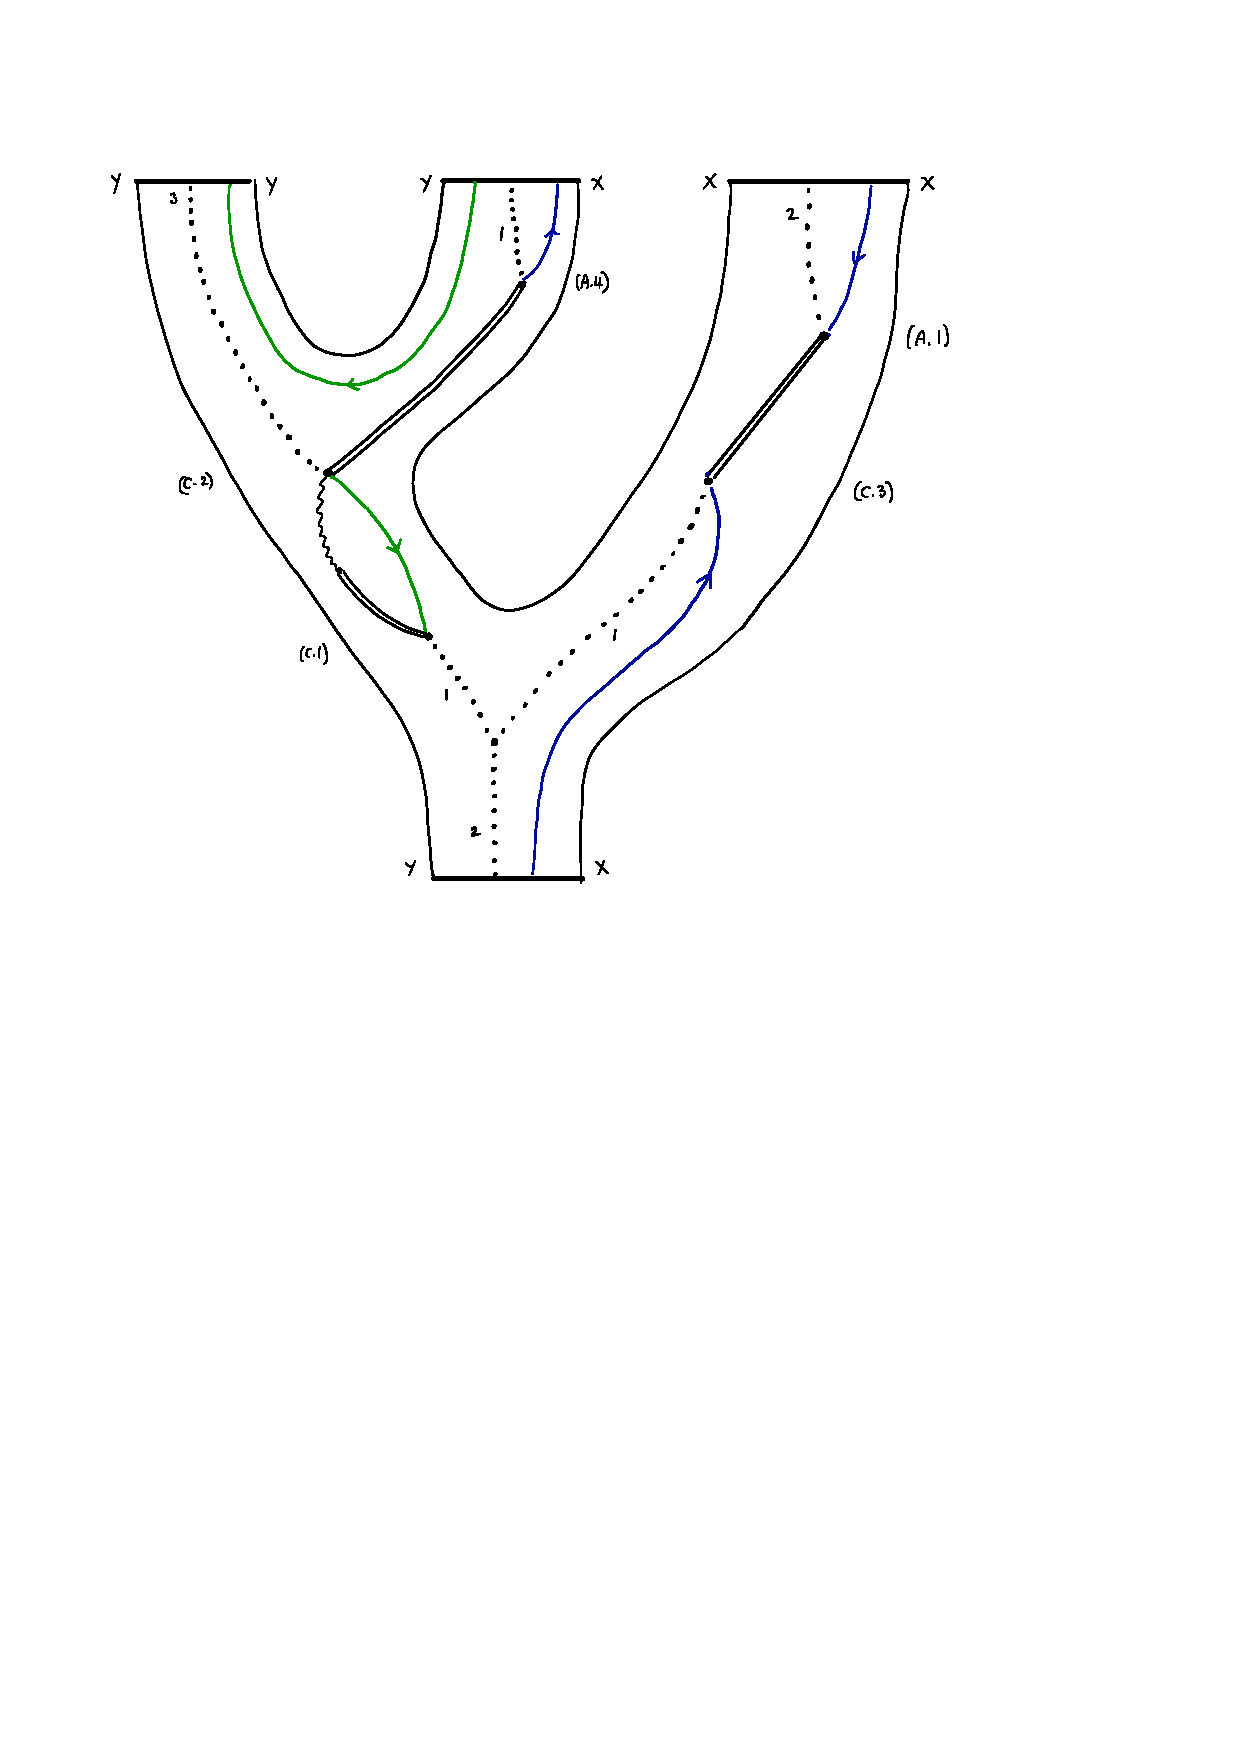
\includegraphics[scale=1.0]{dia16}
\end{center}
\centering
\caption{Example of a Feynman diagram, where blue lines denote $\eta$ and green lines $\xi$.}\label{fig:feynman_1}
\end{figure}
\end{example}
%\[
%\xymatrix@R+2pc{
%R/I \otimes \bigwedge( F_\eta \oplus F_\eta^* ) \otimes R/I \otimes \bigwedge( F_\eta \oplus F_\xi^* ) \otimes R/I \otimes \bigwedge( F_\xi \oplus F_\xi^* ) \ar[d]\\
%R/I \otimes \bigwedge( F_\eta \oplus F_\xi^* )
%}
%\]

%\begin{remark} Comment on the possible pictures in the $m_2$ case. The way to think about these diagrams is a kind of ``off-shell'' extension of the pictures for 2D defect TQFT, where you would also draw this kind of picture for $m_2 \circ (m_2 \otimes 1)$ as a composition map, once you go to cohomology. But there is information in the DG-category that does not survive in the cohomology (e.g. Borromean rings) and this additional structure is recorded in these additional states and their interactions, that give rise to the higher products. This additional information can be interpreted in terms of deformations of potentials, matrix factorisations, and the interaction between the two.
%\end{remark}

%\begin{remark} In special cases there are simplifications: e.g. the $\exp(\delta)$ issues, we can easily identify the kernel of the $e$, etc.
%\end{remark}

\appendix

\section{Formal tubular neighborhoods}\label{section:formaltub}

In this section we introduce the geometric content of the strong deformation retract which forms the basis of this paper, based on the idea of a formal tubular neighborhood \cite{cuntzquillen, lipman}. We begin with a brief introduction to quasi-regular sequences, for more on which see \cite[\S 15.B]{matsumura}, \cite[Chapitre $0$ \S 15.1]{EGA4} and \cite[Section\,10.68]{stacks_project}.

\begin{definition} A sequence $t_1,\ldots,t_n$ in a commutative ring $R$ is \emph{quasi-regular} if, writing $I = (t_1,\ldots,t_n)$, the morphism of $R/I$-algebras
\begin{gather*}
\phi: R/I[z_1,\ldots,z_n] \lto \operatorname{gr}_I R = \bigoplus_{i \ge 0} I^i / I^{i+1}\\
\phi(z_i) = \overline{t_i} \in I/I^2
\end{gather*}
is an isomorphism. In particular, this means that $I/I^2 \cong \bigoplus_{i=1}^n R/I \cdot \overline{t_i}$.
\end{definition}

We recall the motivation for this definition from algebraic geometry.

\begin{remark} Let $Y$ be a Noetherian scheme and let $i: X \lto Y$ be a closed subscheme with ideal sheaf $\mathscr{I}$. The first-order deformations of $X$ in $Y$ are controlled \cite[Theorem VI-29]{eisenbudharris} by the normal sheaf $\mathscr{N}_{X/Y} = \Hom_{\cat{O}_X}(\mathscr{I}/\mathscr{I}^2, \cat{O}_X)$.

In general, the full description of the space of normal directions to $X$ in $Y$ requires more than just the normal sheaf. The correct approach is to start with the blowup $\pi$ of $Y$ along $X$ (which is described by a universal property) and then look at the closed subscheme of that blowup induced by $X$, as in the diagram:
\[
\xymatrix@C+2pc{
\operatorname{Proj}_X( \oplus_{i \ge 0} \mathscr{I}^i/\mathscr{I}^{i+1} ) \ar[r]^-j\ar[d] & \operatorname{Proj}_Y( \oplus_{i \ge 0} \mathscr{I} ) \ar[d]^-{\pi}\\
X \ar[r]_-{i} & Y\,.
}
\]
The closed subscheme $j$ of the blowup (called the strict transform of $X$) is given by the relative Proj of the sheaf of graded algebras $\oplus_{i \ge 0} \mathscr{I}^i/\mathscr{I}^{i+1}$ on $X$, and its points give the correct notion of a point on $X$ together with a normal direction in $Y$. For this reason the scheme $C_X(Y) = \Spec_X( \oplus_{i \ge 0} \mathscr{I}^i / \mathscr{I}^{i+1} )$, whose projectivisation is the strict transform of $X$ in the blowup, is called the \emph{normal cone} of $X$ in $Y$.
\end{remark}

Thus, to say that a sequence $t_1,\ldots,t_n$ is quasi-regular is to say that the projectivised normal cone of $X = \Spec(R/I)$ in $Y = \Spec(R)$ is the space of lines in the normal bundle, since the definition of quasi-regularity gives 
\begin{align*}
\Spec_{Y}( \operatorname{Sym}( \mathscr{N}^*_{X/Y} ) ) &\cong \Spec( \operatorname{Sym}_{R/I}( I/I^2 ) )\\
&= \Spec( R/I[z_1,\ldots,z_n] )\\
&\cong \Spec( \operatorname{gr}_ I R)\\
&= C_X(Y)\,.
\end{align*}
Recall that in differential geometry if we are given a submanifold $X$ of a smooth manifold $Y$ the tubular neighborhood theorem \cite[\S 4.5]{hirsch} identifies an open neighborhood of the zero section of the normal bundle $N_{X/Y} \lto X$ with an open neighborhood of $X$ in $Y$. 

There is no direct analogue of this identification of neighborhoods for a general closed immersion $i: X \lto Y$ of schemes. Let us discuss what such an identification would mean at the level of \emph{formal} neighborhoods in the affine case, assuming that $I = (t_1,\ldots,t_n)$ is generated by a quasi-regular sequence. Completing the normal cone $C_X(Y)$ along the zero section means completing $R/I[z_1,\ldots,z_n]$ in the $(z_1,\ldots,z_n)$-adic topology, while completing $Y$ along $X$ means taking the $I$-adic completion of $R$, so that such an identification would amount to an isomorphism of topological rings
\be\label{eq:formaltubular}
R/I\llbracket z_1,\ldots,z_n \rrbracket \lto \widehat{R}
\ee
where $\widehat{R}$ denotes the $I$-adic completion. It easy to produce examples where this fails:

\begin{example}\label{eq:example_nontub} Let $k$ be a field, $R = k[x]$ and $I = (x^d)$ for $d > 1$. Since the $I$-adic topology is the same as the $(x)$-adic topology, $R/I\llbracket z \rrbracket = k[x]/(x^d) \llbracket z \rrbracket \neq k\llbracket x \rrbracket = \widehat{R}$ since one ring is reduced while the other is not.
\end{example}

However, if $R/I$ is smooth \cite[Definition 28.D]{matsumura}, so that we are in a situation more resembling the one in differential geometry, there is indeed an isomorphism of topological rings of the form \eqref{eq:formaltubular} (see e.g. Lemma \ref{prop_algtube} below). This \emph{formal tubular neighborhood theorem} was developed in the noncommutative setting by Cuntz-Quillen \cite[Theorem 2]{cuntzquillen}. 

In our applications, however, Example \ref{eq:example_nontub} is more typical, as $I$ is generated by the partial derivatives of a potential $W$ and the critical locus $R/I$ of a potential is rarely smooth. While in general there is no strong analogue of the tubular neighborhood theorem, Lipman proves in \cite{lipman} that the cases we care about, there is still an isomorphism of $k\llbracket z_1,\ldots,z_n \rrbracket$-modules, and this is enough to produce connections.

\begin{setup}\label{setup:connection_t} For the rest of this section let $k$ be a commutative $\mathbb{Q}$-algebra, $R$ a $k$-algebra, and let $t_1,\ldots,t_n$ be a quasi-regular sequence in $R$ such that, writing $I = (t_1,\ldots,t_n)$, the quotient $R/I$ is a finitely generated projective $k$-module.
\end{setup}

\begin{lemma}\label{prop_algtube} Any $k$-linear section $\sigma$ of the quotient $\pi: R \lto R/I$ induces an isomorphism of $k\llbracket z_1,\ldots,z_n \rrbracket$-modules
\[
\sigmastar: R/I \otimes k\llbracket z_1,\ldots,z_n \rrbracket \lto \widehat{R}
\]
where $\widehat{R}$ denotes the $I$-adic completion. If further $R/I$ is smooth over $k$ then there exists a section $\sigma$ such that $\sigmastar$ is an isomorphism of topological $k$-algebras.
\end{lemma}
\begin{proof}
This is \cite[Lemma 3.3.2]{lipman}. The map $\sigmastar$ is induced from $\sigma$ by extension of scalars, where $k\llbracket \bold{z} \rrbracket$ acts on $\widehat{R}$ by making $z_i$ act as multiplication by $t_i$. The main point is that every $r \in \widehat{R}$ has a \emph{unique} representation as a power series
\be\label{eq:uniq_decompr}
r = \sum_{M \in \mathbb{N}^n} \sigma(r_M) t^M
\ee
for elements $r_M \in R/I$, and the inverse to $\sigmastar$ sends $r$ to $\sum_M r_M z^M$. The uniqueness of \eqref{eq:uniq_decompr} is a consequence of quasi-regularity, while the existence is proven as follows: given $r \in R$ we have $\pi( r - \sigma(r) ) = 0$ and so there exist $a_1,\ldots,a_n$ with
\be\label{eq:uniq_decompr_choices}
r = \sigma(r) + \sum_{i=1}^n a_i t_i\,.
\ee
Applying the same argument to each $a_i$ yields % see (tkorain1)
\begin{align*}
r &= \sigma(r) + \sum_{i=1}^n \big[ \sigma(a_i) + \sum_{j=1}^n a_{ij} t_j \big] t_i\\
&= \sigma(r) + \sum_{i=1}^n \sigma(a_i) t_i + \sum_{i,j=1}^n a_{ij} t_i t_j\,.
\end{align*}
This process converges in the $I$-adic topology to a series \eqref{eq:uniq_decompr}. If $R/I$ is smooth then by a standard argument \cite{matsumura} we can produce a section $\sigma: R/I \lto \widehat{R}$ which is a morphism of $k$-algebras. It is clear then that $\sigmastar$ is an isomorphism of topological algebras.
\end{proof}

Recall from \cite[\S 8.1.1]{loday} the notion of a connection on a module. As alluded to above, we can use the isomorphism of Lemma \ref{prop_algtube} to produce connections. For a more complete discussion on this point, see \cite[Appendix B]{pushforward}.

\begin{corollary}\label{corollary:nabla_sigma} Associated to any $k$-linear section $\sigma$, there is a $k$-linear connection on $\widehat{R}$ as a $k[\bold{z}]$-module, where $z_i$ acts as multiplication by $t_i$:
\be
\nabla_\sigma: \widehat{R} \lto \widehat{R} \otimes_{k[\bold{z}]} \Omega^1_{k[\bold{z}]/k}\,.
\ee
\end{corollary}
\begin{proof}
The usual partial derivatives give a $k$-linear connection on $k\llbracket \bold{z} \rrbracket$ as a $k[\bold{z}]$-module which extends, by Lemma \ref{prop_algtube}, to a connection on $\widehat{R}$, see \cite[\S 8.1.3]{loday}. In terms of the power series representation \eqref{eq:uniq_decompr} the connection is given by
\be\label{eq:explicit_connection}
\nabla_\sigma(r) = \sum_{j=1}^n \sum_{M \in \mathbb{N}^n} M_j \sigma(r_M) t^{M - e_j} \otimes dz_j
\ee
which completes the proof.
\end{proof}

\begin{definition}
With a section $\sigma$ fixed, we will write $\nabla$ for the associated connection $\nabla_\sigma$. We also introduce $k$-linear operators $\frac{\partial}{\partial z_i}: \widehat{R} \lto \widehat{R}$ by the identity $\nabla = \sum_{j=1}^n \frac{\partial}{\partial z_i} dz_j$. The operators $\frac{\partial}{\partial z_i}$ depend on the choice of section $\sigma$, but we will abuse notation and write
\[
\partial_{t_i} := \frac{\partial}{\partial z_i}: \widehat{R} \lto \widehat{R}\,.
\]
%TODO: Later we use $\nabla$ for the extension to $\Omega^*$.
\end{definition}

\begin{example}\label{example:dt_xd} Let $k$ be a field, $R = k[x]$ and $I = (x^d)$, with $t = x^d$. Choose the $k$-linear section $\sigma: R/I \lto R$ defined by $\sigma(x^i) = x^i$ for $0 \le i \le d - 1$. Then
\[
\partial_t( x^2 + x^{d+1} ) = \partial_t( x^2 \cdot 1 + x \cdot x^d ) = x\,.
\]
\end{example}

In an important class of examples there is an explicit algorithm for computing $r_M$ and thus the derivatives $\partial_{t_i}(r)$ for any element $r \in R$.

\begin{remark}\label{remark:grobner} Suppose that $k$ is a characteristic zero field, and $R = k[x_1,\ldots,x_n]$. Choose a monomial ordering for $R$ and let $G = (g_1,\ldots,g_c)$ be a Gr\"obner basis for $I$, which may be computed from the polynomials $t_1,\ldots,t_n$ by Buchberger's algorithm \cite[\S 2.7]{cox_little_oshea}. Moreover this algorithm also computes an expression $g_i = \sum_{j=1}^n h_{ij} t_j$ for $1 \le i \le c$.

Following the notation of \cite{cox_little_oshea} we write $\Bar{r}^G$ for the remainder on division of $r$ by $G$. This is the unique polynomial with no term divisible by any of the leading terms of the $g_i$, and for which there exists $h \in I$ with $r = h + \Bar{r}^G$ \cite[\S 2.6]{cox_little_oshea}. The generalised Euclidean division algorithm produces $\Bar{r}^G$ together with polynomials $b_1,\ldots,b_c$ such that
\be\label{eq:uniq_decompr_2}
r = \Bar{r}^G + \sum_{i=1}^c b_i g_i = \Bar{r}^G + \sum_{j=1}^n \Big[ \sum_{i=1}^c b_i h_{ij} \Big] t_j\,.
\ee
It is easy to check that the function
\[
\sigma: R/I \lto R\,, \qquad \sigma(r) = \Bar{r}^G
\]
is well-defined and is a $k$-linear section of $\pi$ \cite[Corollary 2, \S 2.6]{cox_little_oshea}. This means that \eqref{eq:uniq_decompr_2} is the desired expression in \eqref{eq:uniq_decompr_choices} used to generate the $r_M$'s. So for example in the case $M = \bold{0} \in \mathbb{N}^n$ we take $r_{\bold{0}} = \Bar{r}^G$ and for $1 \le j \le n$ in the case $M = e_j$ we have
\[
r_{e_j} = \sum_{i=1}^c \overline{b_i h_{ij} }^G\,.
\]
Observe that the monomials $x^\alpha$ with $\alpha$ not divisible by any of the leading terms of the $g_i$ give a $k$-basis of $R/I$. Denote the set of such tuples $\alpha$ by $\Lambda$. Then $R/I = \oplus_{\alpha \in \Lambda} k x^\alpha$ and $\sigma(x^\alpha) = x^\alpha$, generalising Example \ref{example:dt_xd}. 

What we have already said computes the coefficients of $r_M$ in the basis $\{x^\alpha\}_{\alpha \in \Lambda}$ in the cases where $|M| \le 1$. For the cases where $|M| = 2$ we simply have to run the division algorithm with $\sum_{i=1}^c b_i h_{ij}$ in place of $r$ in \eqref{eq:uniq_decompr_2}. Proceeding in this way constitutes an algorithm for computing the coefficient of $x^\alpha$ in $r_M$ for any $M \in \mathbb{N}^n$.
\end{remark}

The upshot is that when $k$ is a field, the map (abusing notation TODO)
\[
(\sigma_{\bold{t}})^{-1}: \widehat{R} \lto R/I \otimes k \llbracket \bold{t} \rrbracket
\]
sends $r \in R$ to a power series $\sum_{M \in \mathbb{N}^n} r_M t^M$ whose coefficients $r_M$ are obtained by \emph{iterated Euclidean division} of $r$ by a Gr\"obner basis of $I$. When $k$ is not a field, it is not obvious how to calculate the $r_M$ in general.

\section{Proofs}\label{section:proofs}
% REF: (ainfmf28) and to a lesser extent (ainfmf29)

In this section we prove Theorem \ref{theorem:main_ainfty_products} and Theorem \ref{theorem:homotopy_clifford}. All notation is as in Setup \ref{setup:overall}, and more generally as in Section \ref{section:the_model}. For example $\AA$ denotes the DG-category of matrix factorisations of $W$ and $\AA_{\theta}$ is the extension of \eqref{eq:defn_AAtheta}. The proofs mostly consist of applying the techniques already developed in \cite{pushforward, cut} to the situation at hand, but there are two technical points worth noting:
\begin{itemize}
\item[(i)] In \cite{cut} the quasi-regular sequence $t_1,\ldots,t_n$ is always $\partial_{x_1} W, \ldots, \partial_{x_n} W$.
\item[(ii)] In \cite{cut} there is an assumption that $k$ is Noetherian.
\end{itemize}
As we explain in Appendix \ref{section:noetherian} the Noetherian hypothesis is not necessary. Regarding (i), we reiterate the relevant parts of \cite{cut} below in the current generality (that is, the hypotheses of Setup \ref{setup:overall}) where $t_i$ is not necessarily $\partial_{x_i} W$. The upshot is that the only place where the hypothesis that $t_i = \partial_{x_i} W$ plays any meaningful role is in the final form of the Clifford operator $\gamma_i^\dagger$ and we address this explicitly in the proof of Theorem \ref{theorem:homotopy_clifford}.

The aim is to put a strict homotopy retract \cite[\S 3.3]{lazaroiu} on $\AA_\theta$, where
\[
\AA_\theta(X,Y) = \bigwedge F_\theta \otimes \Hom_R(X,Y) \otimes_R \widehat{R}\,.
\]
The $I$-adic completion $\widehat{R}$ of $R$ has $t_1,\ldots,t_n$ as a quasi-regular sequence and $\widehat{R}/I \widehat{R} \cong R/I$. By \cite[Appendix B]{pushforward} there is a standard flat $k$-linear connection
\[
\nabla^0: \widehat{R} \lto \widehat{R} \otimes_{k[\bold{t}]} \Omega^1_{k[\bold{t}]/k}
\]
where $k[\bold{t}]$ denotes the polynomial ring in variables $t_i$. Let $X,Y \in \ob(\AA)$. We run through the steps of \cite[\S 4.3]{cut} with $\bigwedge F_\theta$ our new notation for $S_m$, and the complex $\Hom_R(X,Y) \cong X^{\vee} \l Y$ replacing $Y \l X$ (see \cite[\S 4.5]{cut} which also discusses this special case). The role of $k[\bold{y}]$ in \emph{loc.cit} is now played by $R = k[\bold{x}]$. In the first step $\nabla^0$ extends to a $k$-linear operator $\nabla$ on $\widehat{R} \otimes_{k[\bold{t}]} \Omega^*_{k[\bold{t}]/k}$. Choosing a homogeneous $R$-basis for $X,Y$ and taking the induced basis on $\Hom_R(X,Y)$ over $R$, and extending $\nabla$, we get a $k$-linear splitting homotopy
\[
H = [d_K, \nabla]^{-1} \nabla \quad \text{ on the complex } \quad \xymatrix{ \big( K \otimes_R \Hom_R(X,Y) \otimes_R \widehat{R}, d_K \big) }
\]
where $(K,d_k) = \big( \bigwedge F_\theta \otimes R, \sum_{i=1}^n t_i \theta_i^* \big)$ and we identify $\theta_i$ with $dt_i$. This splitting homotopy corresponds to the strong deformation retract (with homotopy $H$)
\[
\xymatrix@C+3pc{
\Big(R/I \otimes_R \Hom_R(X,Y),0\Big) \ar@<-1ex>[r]_-\sigma & \Big( K \otimes_R \Hom_R(X,Y) \otimes_R \widehat{R}, \,\,d_K = \sum_i t_i \theta_i^*\, \Big)\,, \ar@<-1ex>[l]_-\pi
}
\]
In the second step we view $d_{\Hom}$, the differential on $\Hom_R(X,Y)$, as a perturbation and we learn that
\[
\phi_\infty = \sum_{m \ge 0} (-1)^m (H d_{\Hom})^m H
\]
is a $k$-linear splitting homotopy, to which is associated the following $k$-linear strong deformation retract of complexes (with homotopy $\phi_{\infty}$)
\[
\xymatrix@C+3pc@R+3pc{
\Big( R/I \otimes_R \Hom_R(X,Y), d_{\Hom} \Big) \ar@<-1ex>[r]_-{\sigma_\infty} &
\Big( K \otimes_R \Hom_R(X,Y) \otimes_R \widehat{R}, d_K + d_{\Hom} \Big) \ar@<-1ex>[l]_-{\pi}
}
\]
where
\[
\sigma_\infty = \sum_{m \ge 0} (-1)^m (H d_{\Hom})^m \sigma\,.
\]
In the third step, since each $t_i$ acts null-homotopically on $\Hom_R(X,Y)$ we have an isomorphism of complexes over $R$
\[
\xymatrix@C+3pc{
\Big( K \otimes_R \Hom_R(X,Y) \otimes_R \widehat{R}, d_K + d_{\Hom} \Big) \ar@<-1ex>[r]_-{e^{\delta}} & \Big( \bigwedge F_\theta \otimes \Hom_R(X,Y) \otimes_R \widehat{R}, d_{\Hom} \Big)\,, \ar@<-1ex>[l]_-{e^{-\delta}}
}
\]
where $\delta = \sum_{i=1}^n \lambda_i \theta_i^*$. Note we do \emph{not} assume that $\lambda_i$ is a partial derivative of $d_X$. In the fourth step the canonical map $\varepsilon: \Hom_R(X,Y) \lto \Hom_R(X,Y) \otimes_R \widehat{R}$ is by Lemma \ref{lemma:completion_he} (based on \cite[Remark 7.7]{pushforward}) a homotopy equivalence over $k$. Hence we have homotopy equivalences of $k$-complexes, combining the above

\begin{center}
\begin{tabular}{ >{\centering}m{9cm} >{\centering}m{1cm}}
\xymatrix@C+3pc@R+3pc{
\Big( \bigwedge F_\theta \otimes \Hom_R(X,Y), d_{\Hom} \Big) \ar[d]^-{\varepsilon}\\
\Big( \bigwedge F_\theta \otimes \Hom_R(X,Y) \otimes_R \widehat{R}, d_{\Hom} \Big)  \ar@<-2ex>[d]_-{e^{-\delta}}\\
\Big( K \otimes_R \Hom_R(X,Y) \otimes_R \widehat{R}, d_K + d_{\Hom} \Big) \ar@<-2ex>[u]_-{e^{\delta}}\ar@<-2ex>[d]_-{\pi}\\
\Big( R/I \otimes_R \Hom_R(X,Y), \overline{d_{\Hom}} \Big) \ar@<-2ex>[u]_-{\sigma_\infty}
}
&
\tagarray{\label{eq_4_1}}
\end{tabular}
\end{center}
Note that $R/I \otimes_R \Hom_R(X,Y)$ is by our hypotheses a $\nZ_2$-graded complex of finite rank free $k$-modules. Next we argue that \eqref{eq_4_1} gives a strict homotopy retraction of $\AA_{\theta}$. With this in mind the overall content of \eqref{eq_4_1} is a $k$-linear homotopy equivalence
\[
\xymatrix@C+3pc{
\big( \bigwedge F_\theta \otimes \Hom_R(X,Y) \otimes_R \widehat{R}, d_{\Hom} \big) \ar@<-1ex>[r]_-{\Phi} & \big( R/I \otimes_R \Hom_R(X,Y), \overline{d_{\Hom}}\big)\,, \ar@<-1ex>[l]_-{\Phi^{-1}}
}
\]
where we have $\Phi \circ \Phi^{-1} = 1$ and $\Phi^{-1} \circ \Phi = 1 - [d_{\Hom}, \widehat{H}]$ where
\begin{align}
\Phi &= \pi \circ e^{-\delta}\,,\\
\Phi^{-1} &= e^{\delta} \circ \sigma_\infty\,,\\
\widehat{H} &= e^{\delta} \circ \phi_{\infty} \circ e^{-\delta}
\end{align}
By construction we have:

\begin{lemma} The data $(P,G)$ consisting of
\begin{gather*}
P_{X,Y} = \Phi^{-1} \circ \Phi: \AA_\theta(X,Y) \lto \AA_\theta(X,Y)\\
G_{X,Y} = \widehat{H}: \AA_\theta(X,Y) \lto \AA_\theta(X,Y)
\end{gather*}
form a strict homotopy retract on the DG-category $\AA_{\theta}$ in the sense of \cite[\S 3.3]{lazaroiu}.
\end{lemma}

\begin{proof}[Proof of Theorem \ref{theorem:main_ainfty_products}] 
By homological perturbation \cite[\S 3.3, p.33]{lazaroiu} (see also \cite[\S I]{seidel} and particularly \cite[Remark 1.15]{seidel}) applied to the strict homotopy retract of the lemma, we obtain forward suspended $A_\infty$-products $\{ \rho_k \}_{k \ge 1}$ defined on the family of spaces
\[
\xymatrix@C+2pc{
\BB(X,Y) = R/I \otimes_R \Hom_R(X,Y) \ar[r]_-{\cong}^-{\Phi^{-1}} & \operatorname{Im}(P_{X,Y})
}
\]
which make $(\BB, \rho)$ into an $A_\infty$-category. These higher products have the given description in terms of sums over trees. Moreover there are $A_\infty$-functors $F,G$ with $F_1 = \Phi, G_1 = \Phi^{-1}$ and an $A_\infty$-homotopy $G \circ F \simeq 1$, see \cite{markl_transfer}. It remains to check strict unitality. Clearly $\AA_{\theta}$ is strictly unital, since it is a DG-category. Now we apply \cite[p.37]{lazaroiu} which shows that $\BB$ is strictly unital, provided $P_{X,Y} \circ G_{X,Y} = 0$ and $G_{X,X}(u_X) = 0$ for all units $u_X$. The first condition follows because we have a strong deformation retract (not just a strict homotopy retract in the sense of \cite{lazaroiu}) and the second condition because
\[
u_X = 1 \otimes \operatorname{id}_{X,X} \in \bigwedge F_\theta \otimes \Hom_R(X,X) \otimes_R \widehat{R}
\]
and hence $G_{X,X}(u_X) = 0$ since $e^{-\delta}(1 \otimes \operatorname{id}_{X,X}) = 1 \otimes \operatorname{id}_{X,X}$ and $\nabla(1) = 0$.
\end{proof}%By the argument of \cite[Remark 1.13]{seidel} if $k$ is a field we have also an $A_\infty$-homotopy $F \circ G \simeq 1$.
%  Since $\Phi, \Phi^{-1}$ are quasi-isomorphisms, so are $F,G$. 

\begin{proof}[Proof of Theorem \ref{theorem:homotopy_clifford}] We may assume $F_1 = \Phi$ and $G_1 = \Phi^{-1}$ so that by definition $\gamma_i = \Phi \circ \theta_i^* \circ \Phi^{-1}$ and $\gamma^\dagger_i = \Phi \circ \theta_i \circ \Phi^{-1}$. These transfers were studied in \cite{cut} quite generally, but the final formulas were given only in the special case where $t_i = \partial_{x_i} W$, and our job here is to recapitulate the argument to the degree that is necessary to derive the general formula and exhibit that everything we need from \cite{cut} works in full generality.

From \cite[Lemma 4.17]{cut} we get $e^{-\delta} \theta_i^* e^{\delta} = \theta_i^*$ and \cite[Theorem 4.28]{cut} gives
\begin{align*}
e^{-\delta} \theta_i e^{\delta} &= \theta_i - \sum_{m \ge 0} \sum_{q_1,\ldots,q_m} \frac{1}{(m+1)!} \big[ \lambda_{q_m}\,, \big[ \lambda_{q_{m-1}}, \big[ \cdots [ \lambda_{q_1}, \lambda_i ] \cdots \big] \theta^*_{q_1} \cdots \theta^*_{q_m}\\
&= \theta_i - \lambda_i - \frac{1}{2} \sum_q [\lambda_q, \lambda_i] \theta_q^* + \cdots
\end{align*}
Next we copy elements from the proof of \cite[Proposition 4.35]{cut}. Throughout $\At_i$ means $[d_{\Hom}, \partial_{t_i}]$ defined as in \cite{pushforward} with respect to the ring morphism $k[\bold{t}] \lto R$. We now make use of an argument that first appeared in a slightly different form in \cite[(10.3),(10.4)]{pushforward}. Recall $\sigma_\infty = \sum_{m \ge 0} (-1)^m (\zeta \nabla d_{\Hom})^m \sigma$. Now $\nabla \zeta = \zeta \nabla$, $\nabla^2 = 0$ and $\nabla \sigma = 0$ hence we can replace any string $\zeta \nabla d_{\Hom} \cdots \zeta \nabla d_{\Hom} \sigma$ by the string $\zeta [\nabla, d_{\Hom}] \cdots \zeta [\nabla, d_{\Hom}] \sigma$. Hence
\[
\sigma_\infty = \sum_{m \ge 0} (-1)^m \Big\{ \zeta [\nabla, d_{\Hom}] \Big\}^m \sigma\,.
\]
The point of this replacement is that $[\nabla, d_{\Hom}]$ is $k[\bold{t}]$-linear and so, using that as an operator on $\bigwedge F_\theta \otimes R/I \otimes k\llbracket \bold{t} \rrbracket$ the operator $\zeta$ has the property that modulo $(\bold{t}) k\llbracket \bold{t} \rrbracket$
\[
\zeta( \omega \otimes z \otimes f ) = \frac{1}{|\omega|} z \omega \otimes z \otimes f \quad \text{(mod $\bold{t}$)}
\]
we may calculate
\begin{align*}
\pi \theta_{q_1}^* \cdots \theta_{q_m}^* \sigma_\infty &= \sum_{m \ge 0} (-1)^m \pi \theta_{q_1}^* \cdots \theta_{q_m}^* \Big\{ \zeta [\nabla, d_{\Hom}] \Big\}^m \sigma\\
&= \sum_{m \ge 0} (-1)^m \frac{1}{m!} \pi \theta_{q_1}^* \cdots \theta_{q_m}^* \Big\{ \sum_{k=1}^n \theta_k [\partial_{t_k}, d_{\Hom}] \Big\}^m \sigma\\
&= \frac{1}{m!} \sum_{\tau \in S_m} (-1)^{|\tau|} \At_{q_{\tau 1}} \cdots \At_{q_{\tau m}}\,.
\end{align*}
So far this is an \emph{equality} of operators on the complex $\BB(X,Y)$, but we can now apply the fact that Atiyah classes anti-commute up to $k$-linear homotopy (the argument of \cite[Theorem 3.11]{cut} applies) to see that
\[
\pi \theta_{q_1}^* \cdots \theta_{q_m}^* \sigma_\infty \simeq \At_{q_1} \cdots \At_{q_m}\,.
\]
To conclude we apply this to the operators $\gamma_i = \pi e^{-\delta} \theta_i^* e^\delta \sigma_\infty = \pi \theta_i^* \sigma_\infty$ and $\gamma_i^\dagger = \pi e^{-\delta} \theta_i e^\delta \sigma_\infty$ exactly as in \cite[Proposition 4.35]{cut}.
\end{proof}

\section{Removing Noetherian hypotheses}\label{section:noetherian}
% REF: (ainfmf34)

In \cite{cut} there is a hypothesis that the base ring $k$ is Noetherian. This is not necessary, and we explain how to remove it. Along the way we prove Lemma \ref{lemma:completion_he}. Throughout $k$ is a commutative $\mathbb{Q}$-algebra and $R$ a $k$-algebra, and $t_1,\ldots,t_n$ is a quasi-regular sequence in $R$ with $I = (t_1,\ldots,t_n)$. We write $\widehat{R}$ for the $I$-adic completion. It is well-known that the sequence $t_1,\ldots,t_n$ is quasi-regular in $\widehat{R}$ and that the canonical map $R/I \lto \widehat{R}/I\widehat{R}$ is an isomorphism; see for example \cite[\S 15.B]{matsumura}, \cite[Chapitre $0$ \S 15.1]{EGA4}.

\begin{lemma}\label{lemma:trivialsplit} Suppose that
\begin{itemize}
\item[(i)] $R, R/I$ are projective $k$-modules.
\item[(ii)] The Koszul complex $K$ of $t_1,\ldots,t_n$ over $R$ is exact in nonzero degrees.
\end{itemize}
Then if $\sigma: R/I \lto R$ is any $k$-linear section of the quotient map $\pi: R \lto R/I$ and $\pi$ is is the canonical morphism of complexes $\pi: (K,d_K) \lto (R/I,0)$ then there is a degree $-1$ $k$-linear operator $h$ on $K$ as in the diagram
\[
\xymatrix@C+3pc{
(R/I,0) \ar@<-1ex>[r]_-\pi & (K,d_K)\,, \ar@<-1ex>[l]_-\sigma
}\quad h
\]
such that
\begin{itemize}
\item $\pi \sigma = 1$,
\item $\sigma \pi = 1_K - [d_K, h]$
\item $h^2 = 0, h\sigma = 0, \pi h = 0$.
\end{itemize}
\end{lemma}
\begin{proof}
Since $R$ and $R/I$ are projective over $k$, the Koszul complex may be decomposed into a series of \emph{split} short exact sequences, and $h$ is easily constructed from these splittings with the desired properties.
\end{proof}

Next we observe that \cite[Remark 7.7]{pushforward} holds in greater generality. %It is easy to see that everything in \cite[\S 7]{pushforward} holds if $X$ is not necessarily finite rank (but still free).

\begin{remark}\label{remark:fixing_dm} Let $\varphi: S \lto R$ be a ring morphism, $W \in S$ and $(X,d)$ a matrix factorisation of $W$ over $R$ (again, not necessarily finite rank), $t_1,\ldots,t_n$ a quasi-regular sequence in $R$ with $t_i \cdot 1_X \simeq 0$, and homotopies $\lambda_i$. We assume that there is a deformation retract (of $\mathbb{Z}$-graded complexes) over $S$
\be\label{eq:fixing_dm_1}
\xymatrix@C+3pc{
(R/\bold{t} R,0) \ar@<-1ex>[r]_-\pi & (K_R(\bold{t}),d_K)\,, \ar@<-1ex>[l]_-\sigma
}\quad h
\ee
satisfying $h^2 = 0, h \sigma = 0, \pi h = 0$ where $\pi$ is the canonical map. By the previous lemma, it suffices for this to assume that $R,R/I$ are projective over $k$ and that $K_R(\bold{t}) = K$ is exact except in degree zero. Let $\alpha: R \lto R'$ be any ring morphism such that
\begin{itemize}
\item $t_1,\ldots,t_n$ is quasi-regular in $R'$
\item the induced map $R/\bold{t} R \lto R'/\bold{t} R'$ is an isomorphism
\item there is a deformation retract (of $\mathbb{Z}$-graded complexes over $S$)
\be\label{eq:fixing_dm_2}
\xymatrix@C+3pc{
(R'/\bold{t} R',0) \ar@<-1ex>[r]_-{\pi'} & (K_{R'}(\bold{t}), d'_K)\,, \ar@<-1ex>[l]_-{\sigma'}
}\quad h'
\ee
satisfying $(h')^2 = 0, h'\sigma' = 0, \pi' h' = 0$ where $K_{R'}(\bold{t})$ is the Koszul complex over $R'$.
\end{itemize}
Then the canonical morphism of linear factorisations of $W$ over $S$, $\varphi_* X \lto (\alpha \varphi)_* \alpha^* X$ is an $S$-linear homotopy equivalence. Here is the proof (note that we are not assuming $\alpha$ is flat, as is done in \cite[Remark 7.7]{pushforward}). The results of \cite{pushforward} show that we have homotopy equivalences over $S$ (where $X' = X \otimes_R R'$)
\begin{gather*}
\pi: X \otimes_R K_R(\bold{t}) \lto X/\bold{t} X\,,\\
\pi': X' \otimes_{R'} K_{R'}(\bold{t}) \lto X'/\bold{t} X'
\end{gather*}
and the canonical $R$-linear map $X/\bold{t} X \lto X'/\bold{t} X'$ is an isomorphism, by hypothesis. It is clear that the canonical $R$-linear map $X \lto X'$ induces a commutative diagram
\[
\xymatrix@C+2pc{
X \otimes_R K_R(\bold{t}) \ar[d]\ar[r]^-\pi & X/\bold{t} X \ar[d]^-{\cong}\\
X' \otimes_R K_{R'}(\bold{t}) \ar[r]_-{\pi'} & X'/\bold{t} X'
}
\]
hence a homotopy commutative diagram $(\pi = \varepsilon \pi^{-1}, \psi' = \varepsilon \circ (\pi')^{-1}$ in the notation of \cite{pushforward})
\[
\xymatrix@C+2pc{
X/\bold{t} X \ar[d]_-{\cong} \ar[r]^-{\pi^{-1}} & X \otimes_R K_R(\bold{t}) \ar[d] \ar[r]^-\varepsilon & X[n] \ar[d]\\
X'/\bold{t} X' \ar[r]_{(\pi')^{-1}} & X \otimes_R K_{R'}(\bold{t}) \ar[r]_-{\varepsilon} & X'[n]
}
\]
If we produce $\vartheta, \vartheta'$ using the homotopies $\lambda_i, \lambda_i' = \lambda_i \otimes_R R'$ as explained in \cite[\S 4]{pushforward} then it is also clear that the following diagram commutes
\[
\xymatrix@C+5pc{
X[n] \ar[d] \ar[r]^-{\vartheta = (-1)^n \pi \lambda_1 \cdots \lambda_n} & X/\bold{t} X \ar[d]^-{\cong} \\
X'[n] \ar[r]_-{\vartheta' = (-1)^n \pi' \lambda_1' \cdots \lambda_n'} & X'/\bold{t} X'\,.
}
\]
So in summary both squares in the following diagram commute in $\HF(S,W)$
\[
\xymatrix@C+2pc{
X/\bold{t} X \ar[d]_-{\cong} \ar[r]^-{\psi} & X[n] \ar[d] \ar[r]^-\vartheta & X/\bold{t} X \ar[d]\\
X'/\bold{t} X' \ar[r]_-{\psi'} & X'[n] \ar[r]_-{\vartheta'} & X'/\bold{t} X'
}
\]
Now $\psi \vartheta = 1$ and $\psi' \vartheta' = 1$ in the homotopy category, and the above shows that $\vartheta \psi = \vartheta' \psi'$ (identifying $X/\bold{t} X$ with $X'/\bold{t} X'$ as these are isomorphic, not just homotopy equivalent). Since they split the same idempotent, $X, X'$ must be isomorphic in $\HF(S,W)$ and so the middle column in the above diagram is a homotopy equivalence, as claimed.
\end{remark}

In \cite{cut} we assumed the ground ring $k$ was Noetherian. The only reason for this hypothesis was to guarantee that the ring homomorphism $k[\bold{y}] \lto \widehat{k[\bold{y}]}$ is flat, which allows us to use \cite[Remark 7.7]{pushforward} to infer that the canonical map $\varepsilon: Y \otimes_{k[\bold{y}]} X \lto Y \otimes_{k[\bold{y}]} \widehat{k[\bold{y}]} \otimes_{k[\bold{y}]} X$ is a homotopy equivalence, in \cite[\S 4.3]{cut}. Using Remark \ref{remark:fixing_dm} above we explain why everything in \cite{cut} holds for \emph{any} commutative $\mathbb{Q}$-algebra.

We assume we are in the context of \cite[Setup 4.1]{cut} and in particular that $U,V,W$ are potentials in the sense of \cite[Definition 2.4]{lgdual}. Set $t_i = \partial_{y_i} V$ for $1 \le i \le m$. By hypothesis this is a quasi-regular sequence in $R = k[\bold{y}]$, $R/\bold{t} R$ is a finitely generated projective $k$-module, and $K_R(\bold{t})$ is exact outside degree zero. We claim that Remark \ref{remark:fixing_dm} applies to
\begin{gather*}
\varphi: k[\bold{x},\bold{z}] \lto k[\bold{x},\bold{y},\bold{z}], \qquad ( Y \otimes_{k[\bold{y}]} X, d_Y \otimes 1 + 1 \otimes d_X)\\
\alpha: k[\bold{x},\bold{y},\bold{z}] \cong k[\bold{x},\bold{z}] \otimes k[\bold{y}] \lto k[\bold{x},\bold{z}] \otimes \widehat{k[\bold{y}]}
\end{gather*}
We check each of the hypotheses in turn:
\begin{itemize}
\item By Lemma \ref{lemma:trivialsplit} since $R,R/I$ are projective $k$-modules and $K_R(\bold{t})$ is exact outside degree zero we have a deformation retract \eqref{eq:fixing_dm_1} satisfying the necessary conditions.

\item Applying \cite[Appendix B]{pushforward} to the tuple $(k, \widehat{R}, \bold{t})$ gives an isomorphism of $k[\bold{z}]$-modules
\[
\sigmastar: R/I \otimes k[\bold{z}] \lto \widehat{R}\,.
\]
Observe that $R/I \otimes K_{k\llbracket \bold{z} \rrbracket}(\bold{z}) \cong K_{\widehat{R}}(\bold{t})$ via $\sigmastar$ as complexes of $k[\bold{z}]$-modules, and in particular $K_{\widehat{R}}(\bold{t})$ is exact outside degree zero. Moreover using connections we may produce a deformation retract \eqref{eq:fixing_dm_2} of the form required by Remark \ref{remark:fixing_dm}.
\end{itemize}
The conclusion is that in $\HF( k[\bold{x},\bold{z}], U - W)$ the canonical map
\[
Y \otimes_{k[\bold{y}]} X \lto Y \otimes_{k[\bold{y}]} \widehat{k[\bold{y}]} \otimes_{k[\bold{y}]} X\,.
\]
is an isomorphism, as claimed. This removes the Noetherian hypothesis from \cite{cut}.

\begin{proof}[Proof of Lemma \ref{lemma:completion_he}] This is a special case of the above: we apply Remark \ref{remark:fixing_dm} to
\begin{gather*}
\varphi: k \lto k[\bold{x}]\,, \qquad ( \Hom_R(X,Y), d_{\Hom} )\,, \qquad \alpha: k[\bold{x}] \lto \widehat{k[\bold{x}]}
\end{gather*}
Notice that in the above $t_1,\ldots,t_n$ need not be the sequence of partial derivatives, provided it satisfies the conditions set out in Setup \ref{setup:overall}.
\end{proof}

\section{More on connections}

In this section we are in the situation of Setup \ref{setup:connection_t}. The Koszul complex of the sequence $t_1,\ldots,t_n$ over $\widehat{R}$ is $(K, d_K) = \Big( \bigwedge( k \theta_1 \oplus \cdots \oplus k \theta_n ) \otimes \widehat{R}, \,\,\sum_i t_i \theta_i^* \Big)$. By identifying $\theta_i$ with $dz_i$ we identify $K$ with $\widehat{R} \otimes_{k[\bold{z}]} \Omega^*_{k[\bold{z}]/k}$. For the remainder of the section we fix a section $\sigma$ and associated connection $\nabla = \nabla_\sigma$. We have the following $k$-linear operator on $\widehat{R}$:
\be\label{eq:explicitdknabla}
d_K \nabla_\sigma = \sum_i t_i \frac{\partial}{\partial t_i}\,.
\ee
Using \eqref{eq:explicit_connection} we have explicitly $d_K \nabla_\sigma(r) = \sum_{M \in \mathbb{N}^n} |M| \sigma(r_M) t^M$ where $|M| = \sum_{j=1}^n M_j$.

\begin{lemma} If $R/I$ is smooth, $\sigma$ may be chosen such that $d_K \nabla_\sigma$ is a derivation of $\widehat{R}$.
\end{lemma}
\begin{proof}
Suppose $\sigma: R/I \lto \widehat{R}$ is an algebra morphism. Then for $r,s \in R$ we have
\[
\sum_M (rs)_M z^M = \sum_M \sum_{A + B = M} r_As_B z^M\,,
\]
and hence $(rs)_M = \sum_{A+B = M} r_A s_B$. From this the claim follows.
\end{proof}

Recall that for a submanifold $X \subseteq Y$, any tubular neighborhood $f: N_{X/Y} \lto Y$ of $X$ in $Y$ determines an open neighborhood $U = f(N_{X/Y})$ of $X$ and on this open neighborhood a vector field $\mathscr{F} = f_*(\mathscr{E})$ induced by the Euler field $\mathscr{E}$ on $N_{X/Y}$, which is the infinitesimal generator of the scaling action of $\mathbb{R}$ in the fibers. In local coordinates $\mathscr{E} = \sum_i x_i \frac{\partial}{\partial x_i}$ where $x_i$ are the coordinates in the fiber directions. Conversely, the integral curves of the vector field $\mathscr{F}$ determine the tubular neighborhood $f$ \cite[\S 2.3]{burs} and, in particular, $\mathscr{F}$ gives rise to a deformation retract of $U$ onto $X$.

When $R/I$ is smooth, the derivation $d_K \nabla_\sigma$ is in light of \eqref{eq:explicitdknabla} clearly analogous to $\mathscr{F}$. In general $d_K \nabla_\sigma$ will \emph{not} be a derivation, but nonetheless the operators $d_K, \nabla_\sigma$ still give rise to a deformation retract of $\widehat{R}$ onto $R/I$ in a sense that we will make precise below.

\begin{example}\label{example:dt_xd2} In the situation of Example \ref{example:dt_xd} observe that $d_K \nabla = t \frac{\partial}{\partial t}$ is \emph{not} a derivation, as for example $t\frac{\partial}{\partial t}( x^d ) = t$ but $x t \frac{\partial}{\partial t}(x^{d-1}) + t \frac{\partial}{\partial t}(x) x^{d-1} = 0$.
\end{example}

Let us now examine the way in which, in the smooth setting, the vector field $\mathscr{F}$ gives rise to idempotents. The Lie derivative $[-, \mathscr{F}]$ gives rise to an idempotent linear operator on the bundle $TY|_X$ which is a splitting of the exact sequence 
\[
0 \lto TY \lto TX|_Y \lto N_{X,Y} \lto 0\,.
\]
While the Lie derivative with $\mathscr{F}$ gives an idempotent operator on vector fields, it is not idempotent on smooth functions. However, a rescaling of its action on smooth functions does give an idempotent, the corresponding algebra being the following:

\begin{remark} Consider the following diagram of $k$-linear operators
\[
\xymatrix@C+3pc@R+2pc{
\widehat{R} \otimes_{k[\bold{z}]} \Omega^2_{k[\bold{z}]/k} \ar@<0.8ex>[r]^-{d_K} &
\widehat{R} \otimes_{k[\bold{z}]} \Omega^1_{k[\bold{z}]/k} \ar@<0.8ex>[l]^-{\nabla^1_\sigma}\ar@<0.8ex>[r]^-{d_K} & \widehat{R} \ar@<0.8ex>[l]^-{\nabla^0_\sigma} \ar@<0.8ex>[r]^-{\pi} & R/I \ar@<0.8ex>[l]^-{\sigma}
}
\]
where $\pi$ is the quotient map, and $\nabla^*_\sigma$ denotes the extension of $\nabla_\sigma$ to an operator on $\widehat{R} \otimes_{k[\bold{z}]} \Omega^*_{k[\bold{z}]/k}$. It is easy to check that
\[
\left( d_K \nabla^1_\sigma + \nabla^0_\sigma d_K \right)\left( \sum_N \sigma(s_N)t^N \otimes dz_j \right) = \sum_N (1 + |N|) \sigma(s_N) t^N \otimes dz_j\,,
\]
and hence $d_K \left( d_K \nabla^1_\sigma + \nabla^0_\sigma d_K \right)^{-1} \nabla^0_\sigma(r) = r - \sigma(r_0)$. So while $d_K \nabla^0_\sigma$ is not an idempotent operator on $\widehat{R}$, the rescaled operator $d_K \left( d_K \nabla^1_\sigma + \nabla^0_\sigma d_K \right)^{-1} \nabla^0_\sigma$ is an idempotent, which splits $\widehat{R}$ as a $k$-linear direct sum $\widehat{R} \cong R/I \oplus I$.
\end{remark}

\section{Operator decorated trees}

Here we collect some standard material on decorated trees. A \emph{tree} is a connected acyclic unoriented graph. All our trees are finite. A \emph{rooted tree} is a tree in which a particular leaf vertex (meaning a vertex of valency $1$) has been designated the root. We view a rooted tree as an oriented graph by orienting all edges towards the root, that is, in the direction of the unique path to the root. The \emph{children} of a vertex $v$ are those vertices $w$ for which $v$ is the next vertex on the path from $w$ to the root. If $w$ is a child of $v$ we call $v$ the \emph{parent} of $w$. A \emph{plane} tree is a rooted tree together with a chosen linear order $w_1,\ldots,w_n$ for the set of children of each vertex $v$. A \emph{morphism} of plane trees is a morphism of oriented graphs which preserves the root vertex and the ordering on children. A plane tree is \emph{valid} if it has $n + 1$ leaves (including the root) for some $n \ge 2$ and all non-leaves have valency at least three. We call leaves \emph{external vertices}, non-leaves \emph{internal vertices}, the edges meeting a leaf are \emph{external edges} and the others are \emph{internal edges}.

\begin{definition} $\cat{T}_n$ is the set of isomorphism classes of valid plane trees with $n + 1$ leaves. We denote by $\cat{BT}_n$ the set of isomorphism classes of valid plane \emph{binary} trees, that is, trees in which every non-leaf vertex has valency three.
\end{definition}

\begin{definition} Let $S$ be a commutative, associative (but not necessarily unital) ring and $Q$ a plane tree. A \emph{decoration} of $Q$ is the following data, where ``graded'' means $\nZ$ or $\nZ_2$-graded (we assume $Q$ has at least one edge):
\begin{itemize}
\item a graded $S$-modules $L_v$ for each leaf $v$ (including the root)
\item a graded $S$-module $M_e$ for each edge $e$
\item for each internal vertex $v$ with incoming edges (in order) $e_1,\ldots,e_k$ and outgoing edge $e$ an integer $N_v$ (in $\nZ$ or $\nZ_2$) and a degree $N_v$ $S$-linear map
\[
\phi_v: M_{e_1} \otimes_S \cdots \otimes_S M_{e_k} \lto M_e
\]
\item for each non-root leaf vertex $l$ a degree zero $S$-linear map $\phi_l: L_l \lto M_e$ where $e$ is incident at $l$
\item a degree zero $S$-linear map $\phi_r: M_e \lto L_r$ where $e$ is incident at $r$, the root vertex.
\end{itemize}
\end{definition}


\bibliographystyle{amsalpha}
\providecommand{\bysame}{\leavevmode\hbox to3em{\hrulefill}\thinspace}
\providecommand{\href}[2]{#2}
\begin{thebibliography}{BHLS03}
  
\bibitem{d0904.4713}
T.~Dyckerhoff, \textsl{Compact generators in categories of matrix factorizations},
  Duke Math. J. \textbf{159} (2011), 223--274,
  \href{http://arxiv.org/abs/0904.4713}{[arXiv:0904.4713]}.
  
\bibitem{lazaroiu}
C.~I.~Lazaroiu, \textsl{Generating the superpotential on a D-brane category: I}, [arXiv:hep-th/0610120].

\bibitem{lazaroiu2}
C.~I.~Lazaroiu, \textsl{String field theory and brane superpotentials}.
  
\bibitem{cut}
D.~Murfet, \textsl{The cut operation on matrix factorisations}, \href{http://arxiv.org/abs/1402.4541}{[arXiv:1402.4541]}.

\bibitem{lgdual}
N.~Carqueville and D.~Murfet, \textsl{Adjunctions and defects in Landau-Ginzburg models}, Adv. Math. \textbf{289} (2016), 480--566.

\bibitem{pushforward}
T.~Dyckerhoff and D.~Murfet, \textsl{Pushing forward matrix factorisations}, Duke Math. J. \textbf{162} (2013), 1249--1311.

\bibitem{weinberg}
Weinberg, \textsl{The Quantum Theory of Fields Volume 1}.

\bibitem{ps}
Peskin \& Shroeder, \textsl{An introduction to QFT}.

\bibitem{sullivan}
D.~Sullivan, \textsl{Open and closed string field theory interpreted in classical algebraic topology} London Math. Soc. Lecture Note Series 308 (2004).

\bibitem{qftstring}
P.~Deligne et al, \textsl{Quantum fields and strings}

\bibitem{EGA4}
A.~Grothendieck, \textsl{\'{E}l\'ements de g\'eom\'etrie alg\'ebrique. {IV}. \'{E}tude
  locale des sch\'emas et des morphismes de sch\'emas}, Inst.~Hautes \'Etudes
  Sci.~Publ.~Math.~(1964), no.~20.

\bibitem{stacks_project}
The Stacks Project, \href{http://stacks.math.columbia.edu/}{http://stacks.math.columbia.edu}.

\bibitem{matsumura}
Matsumura, \emph{book}.

\bibitem{eisenbudharris}
D.~Eisenbud and J.~Harris, \textsl{The geometry of schemes}, Vol. 197. Springer Science \& Business Media, 2006.

\bibitem{cuntzquillen}
J.~Cuntz and D.~Quillen, \textsl{Algebra extensions and nonsingularity}, Journal of the AMS \textbf{8}, No. 2 (1995).

\bibitem{lipman}
J.~Lipman, \textsl{Residues and traces of differential forms via {H}ochschild
  homology}, Contemporary Mathematics \textbf{61}, American Mathematical Society,
  Providence, 1987.

\bibitem{burs}
Burszytn et al, \textsl{Splitting theorems for Poisson and related structures}.

\bibitem{hirsch}
Hirsch, \textsl{Differential topology}.

\bibitem{constructat}
J.~Rubio and F.~Sergeraert, \textsl{Constructive algebraic topology}, Bulletin des Sciences Math\'ematiques 126.5 (2002), 389--412.

\bibitem{constructat2}
J.~Rubio and F.~Sergeraert, \textsl{Constructive homological algebra and applications}, arXiv preprint arXiv:1208.3816 (2012).

\bibitem{loday}
J.-L. Loday, \textsl{Cyclic homology}, Springer, 1997.

\bibitem{markl_transfer}
M.~Markl, \textsl{Transferring $A_\infty$ (strongly homotopy associative) structures}, arXiv preprint math/0401007 (2014).

\bibitem{cox_little_oshea}
Cox, Little, O'shea

\bibitem{lambek_book}
J.~Lambek, \textsl{Lectures on rings and modules}, Vol. 283, American Mathematical Society, 1966.

\bibitem{seidel}
P.Seidel, \textsl{Fukaya Categories and Picard–Lefschetz Theory}

\bibitem{fukaya}
K. Fukaya, \textsl{Floer homology and mirror symmetry. II}, in Minimal surfaces, geometric analysis and symplectic geometry (Baltimore, MD, 1999), Adv. Stud. Pure Math. 34, Math. Soc. Japan, Tokyo, 2002, pp. 31–127.

%\bibitem{fulton}
%W.~Fulton, \textsl{Intersection theory}, Vol. 2. Springer, 1998.

\end{thebibliography}

\end{document}
